\documentclass[12pt,a4paper]{article}


\usepackage{graphicx}
\usepackage{amsmath}
\usepackage{amssymb}
\usepackage{verbatim}
\usepackage{hhline}
\usepackage[absolute]{textpos}
\usepackage[T1]{fontenc}
\usepackage[left=20.0mm, right=30.0mm, top=50mm, bottom=20mm, headheight=45mm,  footskip= 12mm, headsep=6mm, marginparsep=0mm]{geometry}
\usepackage{graphicx}
\usepackage{xcoffins,calc,xcolor} % added
\usepackage[many]{tcolorbox}
\usepackage{fancyhdr}
\usepackage[backend=biber, style=nature]{biblatex}
\usepackage{tabularx}
\usepackage{fancybox}
\usepackage{fancyhdr}
\usepackage{xr}
\usepackage{multicol}
\usepackage{fancyhdr}
\usepackage{lipsum}
\usepackage{adjustbox}
\usepackage{mathtools,tikz,caption}
\captionsetup{labelfont=sc,labelsep=period}
\DeclareRobustCommand\sampleline[1]{%
  \tikz\draw[#1] (0,0) (0,\the\dimexpr\fontdimen22\textfont2\relax)
  -- (2em,\the\dimexpr\fontdimen22\textfont2\relax);%
}
\usepackage{longtable}
\usepackage{caption}
\usepackage{makecell}

\captionsetup[figure]{font=small}

% Define header and footer
\pagestyle{fancy}
\fancyhf{} % Clear all header and footer fields
\fancyhead[L]{\leftmark} % Section title on the left
\fancyhead[R]{\thepage} % Page number on the right
\renewcommand{\headrulewidth}{0.4pt} % Header rule


\addbibresource{lib.bib}

\begin{document}

\begin{titlepage}
    \begin{center}
	{\Large\textbf{Universität Heidelberg}\par}
    {\Large\textbf{Interdisciplinary Center for Scientific Computing} \par}
    {\Large\textbf{Engineering Mathematics and Computing Lab}\par}
	\vspace{3cm}
	{\Large\textbf{Bachelor Thesis}\par}
    \vspace{1cm}
	{\Huge\bfseries Continuous Modeling of Extracellular Matrix Invasion by Tumor Growth  \par}
    \end{center}
    \vspace{6cm}
	
    \raggedright{\Large Name: Maximilian Bing\par}
    {\Large Matriculation number: 3606060\par}
    {\Large Advisor: Professor Vincent Heuveline\par}
    {\Large Date of submission: \today\par}
\end{titlepage}
\vspace*{\fill}  
Hiermit versicher ich, dass ich die Arbeit selbst verfasst und keine anderen als die 
angegebenen Quellen und Hilfsmittel benutzt und wörtlich oder inhaltlich aus fremden 
Werken Übernommenes als fremd kenntlich gemacht habe. Ferner versichere ich, dass die
übermittelte elektronische Version in Inhalt und Wortlaut mit der gedruckten Version
meiner Arbeit vollständig übereinstimmt. Ich bin einverstanden, dass diese
elektronische Fassung universitätsintern anhand einer Plagiatssoftware auf Plagiate
überprüft wird.

\vspace{1cm}


\par\noindent\rule{0.3\textwidth}{0.1pt}
\newline
Abgabedatum:
\vspace*{\fill}
\section*{Zusammenfassung}

Krebszellen können sich vom Primärtumor lösen und das umgebende Gewebe abbauen. 
Kontinuierliche mathematische Modelle wurden in der Vergangenheit mehrmals verwendet, um diesen Prozess besser zu verstehen. In diesem Zusammenhang basieren die Modelle in der Regel auf mindestens drei Schlüsselkomponenten: den Tumorzellen, dem umgebenden Gewebe oder der extrazellulären Matrix (ECM) und den matrixabbauenden Enzymen (MDE). \\ \\
Diese Arbeit untersucht zwei solche kontinuerliches Modell und analysiert den Einfluss der Parameter als auch der Dimension auf die Ergebnisse einer Simulation.
Der Unterschied der beiden analysierten Modelle besteht darin, dass das erste Modell Proliferation der Tumorzellen und Erneuerung der extrazellulären Matrix vernachlaessigt, waehrend das zweite diese biologischen Faktoren beruecksichtigt. 
Da in der Literatur fast ausschlieslich eindimensionalen Versuche zu den Modellen durchgeführt wurden, werden die Experimente hier nur in hoeheren Dimensionen durchgeführt. \\ \\
Darüber hinaus wurde in der Literatur die homogene Struktur der extrazellulären Matrix (ECM) bereits behandelt, jedoch fuer eine heterogene extrazelluläre Matrix Struktur nur solche Faelle analysiert, die wenig biologische Relevany haben. Die Struktur der epithelialen Schicht und der benachbarten extrazellulären Matrix ist jedoch in biologischem Gewebe organisierter als in den spaeter gezeigten Simulationen und anderen Beispielen. \\ \\
Das Ziel dieser Arbeit ist es, einerseits die Parameter und das Modell für höhere Dimensionen zu untersuchen und andererseits eine einfache Heterogenität der ECM-Struktur in Betracht zu ziehen. Wie sie sehen werden haben einige Parameter gewichtigeren Einfluss auf die Ergebnisse als andere, zudem variieren die Groessenordnungen und damit auch die Einflussbereiche der Variablen stark. Eine beretis einfache heterogene Struktur der extrazellulären Matrix anzunehmen veraendert die Ergebnisse ebenfalls stark, da diese entscheidend ist fuer die Bewegung der Tumorzellen im Gewebe.

$\textcolor{red}{heterogenous-ECM-results}$

\clearpage
\section*{Abstract}
Cancer cells can migrate from the primary tumor and degrade the surrounding tissue. Continuous mathematical models have been used several times in the past to better understand this process. In this context, the model is usually based on at least three key species, the tumor cells, the surrounding tissue or extracellular matrix (ECM) and the matrix degradative enzymes (MDE). The investigated model in this work describes the above mentioned 3 parameters, with zero-flux boundry conditions. \\ \\
The analysis of this models is mostly done in $1D$ in the literature and individual examples were done in 2D. However, reproductions of the model show that higher dimensions produce significantly different results. The question therefore arises as to whether the parameters for this model need to 
be selected differently for simulations in 2D or 3D, or whether the results and analysis for the one dimensional case is incorrect. \\
Ergebnis einfuegen\\ \\
Furthermore, the heterogeneous ECM structure has been addressed in the literature. However, the structure of the epithelial layer and the adjacent extracellular matrix is more organized in biological tissue than in the later shown simulations shown and other examples. Therefore, simpler subdivisions of the geometry into ECM tissue could provide more meaningful results. \\ \\
The aim of this work is to investigate the parameters and the model for higher dimensions on the one hand, and to consider a simple heterogeneity of the ECM structure on the other hand. As you will see some parameters have a stronger impact on the results than others, with also varying scale and reach of influence.

$\textcolor{red}{heterogenous-ECM-results}$
\tableofcontents
\newpage
%\listoffigures
%\listoftables
\newpage
%\begin{multicols}{2}
\section{Introduction}
Modelling tumor growth plays a key role in understanding the complex mechanisms, 
governing development and progression of cancer diseases. Since cancer is one of the 
leading death causes worldwide and many of its forms are incurable, challenges in the area of 
Oncology require researchers to have a deep understanding in as well the biological foundation, 
which lead to malignant cell mutation and factors for tumor growing and spreading, as well as the 
mathematical models used for simulating these events. This Bachelorthesis is dedicated to 
analyse Anderson et al.'s \cite*{anderson_continuous_1998,anderson_mathematical_2000} model for 
tumor modelling.\newline
The dynamics of tumerous growth are an intricate system, which is influenced by numerous biological and 
chemical factors, as well as genetic pre-dispostitions, the surrouding tissue of cancer cells, angiogene 
processes an interactions with the immune system. The integration of these factors in mathematical models
allow us to decode these complex interactions with quantification and help us understand the fundamental 
mechanisms, which surroud cancerous diseases, as the last year's experience has shown. \newline 
Mathematical models are a very important part in Oncology. They are used to quantify biological phenomena and 
therefore help to predict and understand tumor development and treatment response. In Mathematical Oncology 
we differentiate between continuous, discrete and hybrid models. For the continuous type, cells and tissue are 
described over time with differential equations modelling continuous quantities like in our case the cell or extracellular matrix density. 
In the discreate case, a entity based model is used, pursued with the goal to better understand the phenoma on cell level.
This approach allows the researcher to better implement biological effects a cell has with its outer circumstances, like interaction 
with other cells, nutrients or other microorganisms. As the name implies do these models use discrete values to describe the temporal 
course of events. Hybrid models try to combine both approaches, to offer efficient systems capturing cell level events 
as well as continuous changes in outer circumstances.
\newline In this work we are investigating how a continuous model proposed by 
Anderson et al. \cite{anderson_continuous_1998,anderson_mathematical_2000} to analyse tumur development in the early stages
performs in the case of different dimensions and free parameter values. 
The model examines the first two stages of a cancer disease; tumor initiaition, where 
the tumor cells are localized to a small area and have not yet spread throughout 
the body; and tumor promotion, with the tumor cells growing and proliferating, invading the 
surrounding tissue.
From examples of the original paper we can already see that the model's results vary with the 
dimensionality of the space we are modelling the partial differential equations in. 
Our main focuse lies on comparing simulations of two dimensions with those of three dimensions 
of extracellular matrix invasion by the tumor growth.
Additionally to the variation of dimensions we will have a closer look on how 
the geometry of the extracellular matrix will influence the tumor development. \newline 
Another point fo interest is the investigation of how the model's free parameters influence the 
tumor dynamics growth. An important task is to give those parameters a biological meaning and 
to eventually gain insight to how to adjust them to make the simulation more realistic.
\section{Theoretical Basics}
\label{sec:theoretical_basics}
\subsection{Basics of Tumor Biology}
\begin{figure}[h]
    \centering
    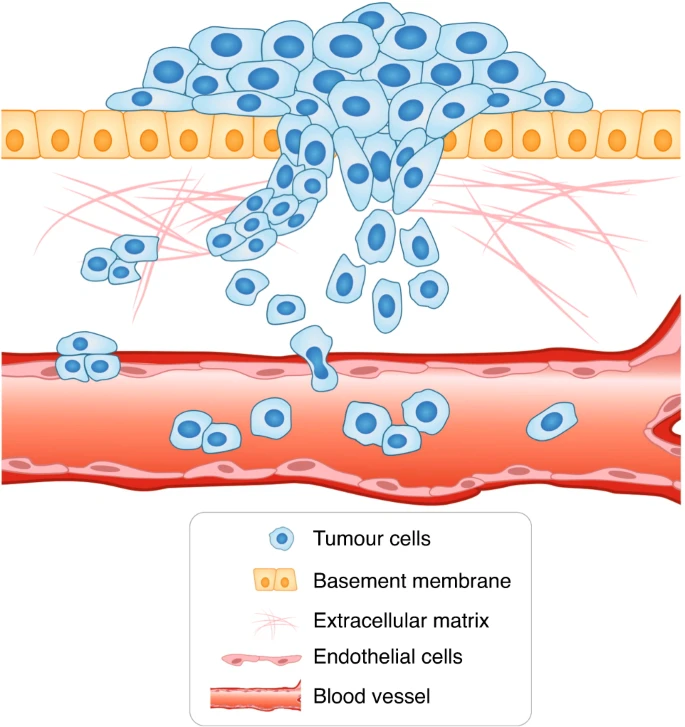
\includegraphics[width=0.85\textwidth]{resources/images/tumour_invasion_stage.png}
    \caption{Tumor Invasion Stage}
    \label{fig:tumor_invasion_stage}
\end{figure}

The body of a living creature is made up of more than 200 different types of cells; the coordination between the cells and their surroundings keeps the body running. Each of these cells is built from the genetic information encoded in the DNA in the cells' nuclei. Though the nucleotide sequence of DNA is well-checked and maintained throughout the cell's life, mutations still occur that cause changes in a cell's DNA. These mutations may be of a positive, negative, or neutral nature. In the case of a harmful mutation, this alternation of the DNA may cause diseases, with cancer being one of them. The failure of the complex system managing cell birth, proliferation, and cell death (apoptosis) causes cancer, resulting in uncontrolled cell proliferation in a local area. A conglomeration of cancer cells is called a tumor. 

Cancer diseases can be categorized medically into five stages. First is the tumor initiation phase, where it comes to the above explained genetic mutations of normal cells. The next stage is the tumor promotion stage, in which the mutated cells of phase one may experience further genetic alterations resulting from uncontrolled growth and proliferation of the cancerous cells. The third stage is the tumor progression stage, where the cancerous cells progress in growing and proliferating, reaching a critical mass, and forming a tumor at a local site of the body. Fourth comes the invasion stage, shown in figure~\ref{fig:tumor_invasion_stage}. Here, the tumor can invade surrounding tissue by breaking through the cellular membrane, invading the extracellular matrix inside, and entering the blood circulation or lymphatic systems. Next, the tumor cells that have invaded the blood circulation of the lymphatic system spread throughout the body and form new tumors. This stage is called Metastization. To grow tumors further, they need access to nutrients and oxygen. During angiogenesis, a tumor develops its own blood vessels, securing its nutritional provision. At this stage, the first symptoms of the host may appear, enabling medical treatment.

In our model, the focus lies on the first two stages: tumor invasion and tumor progression. The tumor invasion stage is characterized by the malignant cells gaining the ability to penetrate and invade the surrounding tissue. The tumor cells break through the normal tissue barrier and infiltrate neighboring structures. In order to do so, the cancer cells produce so-called matrix-degrading enzymes which break down the extracellular matrix. The degradation of the extracellular matrix helps local spreading and destroys otherwise healthy tissue and cells in the affected area. In the next phase, the tumor progression stage, the tumor has grown more extensive, and the cancerous cells take on more aggressive behavior by invading the surrounding area further. While they keep growing uncontrolled, they are also affected by further genetic instabilities, which lead to more mutations, possibly developing resistance mechanisms against, for example, degrading factors. Already in this stage, the affected area is exposed to heavy tissue damage and functional disabilities.

The most important factors influencing those two phases are the genetic dispositions of the tumor cells towards proliferation and the evasion of apoptosis, programmed cell death, which increase the invasive potential. Another critical factor is the geometry of the extracellular matrix, as well as the exact macromolecules that make it up. A solid immune biological defense reaction also helps the body defend against spreading cancer cells. Hence, evasion of detection and destruction of the tumor cells plays a vital role in the first stages. To invade the affected area, the malignant cells need to be able to move freely and quickly. In order to do so, cancer cells can gain the ability to lose adhesion properties, which healthy cells usually have, to allow migrating into the surrounding tissue.
\begin{figure}[h]
    \centering
    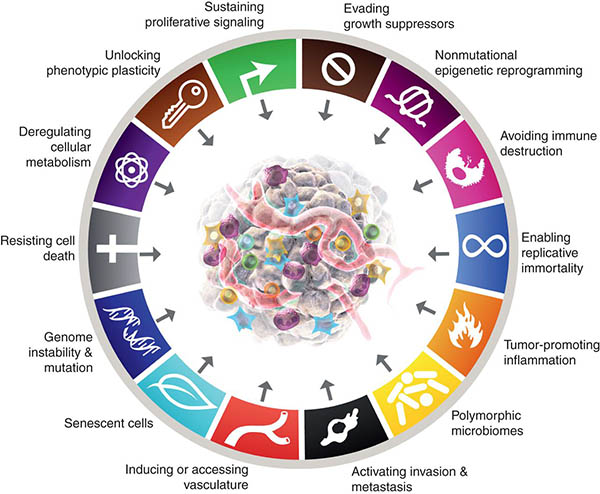
\includegraphics[width=0.85\textwidth]{resources/images/Hallmarks-of-Cancer.jpg}
    \caption{Hallmarks of Cancer}
    \label{fig:hallmarks_of_cancer}
\end{figure}
Another organization principle for cancerous diseases is found in the Hallmarks of cancer,~\ref{fig:hallmarks_of_cancer}, of Douglas Hanahan and Robert Weinberg~\cite{10.1158/2159-8290.CD-21-1059}. They describe a set of functional capabilities, eight hallmark capabilities, and two enabling characteristics commonly acquired by cancer cells. They contribute to their ability to grow uncontrollably, evade the immune system, and metastasize. These hallmarks are sustaining proliferative signaling, evading growth suppressors, avoiding immune destruction, enabling replicative immortality, tumor-promoting inflammation, activating invasion and Metastization, inducing or accessing vasculature, genome instability and mutation, resisting cell death, deregulating cellular metabolism. These Hallmarks of Cancer together contribute to the development and progression of cancer and provide targets for therapeutic intervention and research efforts aimed at understanding and treating the disease. 

In our model, we see many of the capabilities incorporated. Proliferative signaling only relies on the tumor cells themselves and not on typically other hormones or molecules, allowing them to proliferate rapidly without external growth signals. Immune destruction and induced cell death are avoided, optimizing them to survive and accumulate genetic mutations that promote tumor growth. The tumor cells can invade the surrounding tissue, modeled by the extracellular matrix.

\subsection{Mathematical Methods in Oncology}
Mathematical methods and models in Oncology play a crucial role in analyzing, understanding, and predicting cancer development. Since the objective of this research underlies complex and intricate biochemical systems and mechanisms, many models exist that find their respective applications in distinct areas of this research field. These methods can be coarsely divided into three sections: continuous, discrete, and hybrid models~\cite{BEKISZ2020101198}; for describing tumor growth, exponential and logistic growth models are often used, the latter allowing limiting factors to play a role during modeling. These methods are a subclass of the differential equations approach, which bases their functionality on an ordinary or partial differential equation, studying the continuous approach. Like our model, they are not limited to only one equation but can include many, incorporating systematic dependencies on other factors. These models generally deal with continuous quantities like densities or concentrations, for example, spatial and temporal nutritional supply or drug concentration, as well as their effects on the affected area over time. Discrete models use discrete entities to describe the behavior of tumor cells and their interactions with surrounding tissue. They allow us to model a wide range of biological and chemical processes which are hard to describe continuously. Commonly used types in mathematical oncology are, for example, Cellular Automata or Agent-Based Models. Cellular Automata represents cells as entities with states on a grid, with each cell being allowed to change states according to a set of rules based on its own current state and the states of the neighbors.

In contrast, Agent-Based Models enable the differentiation of cell types and allow movement that is not restricted to a grid, implementing complex mechanics at cell-cell or cell-environment levels. Using these discrete models allows researchers to focus on biological effects during modeling, which are hard to describe in continuous models. With these approaches, we can simulate genetic and evolutionary events. For example, they are studying the genetic alternations of tumor cells or the interaction between healthy and cancerous cells.

Hybrid models combine both methods above, using continuous and discrete approaches. Like in the model proposed by Franssen et al.~\cite{franssen_mathematical_2019} or Anderson et al.~\cite{anderson_continuous_1998}, these approaches allow to incorporate the exactness of continuous models with a wide range of biological effects described by discrete models.

However, not all models try to model tumor growth; others are concerned with optimality regarding drug dosages or radiation exposition, offering personalized treatment, or Machine Learining and Data Mining methods analyzing large datasets to identify patterns and predict outcomes. The latter method may be used in all kinds of applications, for example, spacial or temporal cancer development, as well as drug dosage optimization for individual patients. Putting all these methods together gives us a powerful toolbox to simulate and understand cancer biology. As the last years have shown, they are applied in a wide range of areas, offering insight into all areas of cancer research. Therefore, it is essential to come up with methods and evaluate their usefulness and meaningfulness in different research areas.
\section{Modelling}

\subsection{Mathematical Formulation}

The model propsed by Anderson et al. \cite{anderson_continuous_1998,anderson_mathematical_2000} 
and Chaplain et al. \cite{anderson_continuous_1998,chaplain_mathematical_2006,chaplain_mathematical_2006-1,franssen_mathematical_2019}, extended with terms for cell modelling cell proliferation consists of a system of linearly coupled partial differential equations: 

\begin{align}
	\frac{\partial c}{\partial t} &= D_c \Delta c - \chi \nabla \cdot (c\nabla e)  + \mu_1 c\left(1-\frac{c}{c_0}-\frac{e}{e_0}\right)\label{eq1}\\
	\frac{\partial e}{\partial t} &= -\delta m e  + \mu_2 c\left(1-\frac{c}{c_0}-\frac{e}{e_0}\right)\label{eq2}\\
	\frac{\partial m}{\partial t} &= D_m \Delta c + \mu_3 c - \lambda m\label{eq3}
\end{align}
with zero-flux boundary conditions, 
\begin{align}
	n\cdot (-D_c \nabla c + c \chi\nabla e) &= 0 \label{eq4}\\
	n \cdot (-D_m\nabla m ) &= 0\label{eq5}
\end{align}

where the free parameters are $D_c$, $D_m$, $\chi$, $\delta$, $\mu_1$, $\mu_2$, $\mu_3$ and $\lambda$. \newline
The variable $c$ describes the tumor cell density, $e$ the density of the extracellular matrix and $m$ the matrix-degrading enzyme concentration. All of those functions are mathematically defined to be mapping a 1,2 or 3 dimensional spacial value and a point in time to a scalar value describing the concentration at a specific point in space and time, $\{c,e,m\} : \mathbb{R}^{3} \times \mathbb{R} \rightarrow \mathbb{R}$.\newline
To derive at the expression for the tumor cell concentration $c$ we are going to assume that the tumor cell's moement is subject to two influences, haptotaxis and random movement. Haptotaxis is a directed migratory response of cells to gradients of fixed or bound chemicals \cite{anderson_continuous_1998} and random movement is influenced by for example mechanical stress, electric voltage or other such physical effects. To get an expression for how much or how fast the tumor cells move, we need to define what flux is, flux is defined to be the amount of a substance  which crosses a unit area in unit time. Incorporating the two assumed influencing factors into our mathematical model we define the haptotatic flux $J_{hapto} = \chi c \nabla e$, where $\chi$ is the haptotactic flux coefficient, and the random flux $J_{random} = -D_c \nabla c$, where $D_c$ is random mobility constant. In general this parameter could also be a function of both extracellular matrix and matrix-degrading enzyme concentration $D_c \rightarrow D(e,m)$. As we know cells proliferate and grow over time, so we want to respect this in our model with a term for tumor cell proliferation: $\mu_1 c (1-\frac{c}{c_0} - \frac{e}{e_0})$. The idea is that this term describes the cell proliferation with a logisitic growth model, $\mu_1$ describing the proliferation rate.
In the inital model proposed by Anderson et al. \cite{anderson_continuous_1998,anderson_mathematical_2000} 
and Chaplain et al. \cite{anderson_continuous_1998,chaplain_mathematical_2006,chaplain_mathematical_2006-1,franssen_mathematical_2019}, they did not respect proliferation of tumor cells and extracellular matrix and therefore applied a conservation equation for the tumor cells $\frac{\partial c}{\partial t} + \nabla \cdot (J_{hapto} + J_{random}) = 0$, in our model we extend this conservation formula with a proliferation rate. Explicitly inserting the flux formulas and logisitc growth function for the tumor cells gives us: $\frac{\partial c}{\partial t} + \nabla (J_{hapto} + J_{random}) + \mu_1 c (1-\frac{c}{c_0} - \frac{e}{e_0}) = \frac{\partial c}{\partial t} + \chi \nabla (c \nabla e) - D_c \Delta c + \mu_1 c (1-\frac{c}{c_0} - \frac{e}{e_0})$. Which is equivalent to equation \ref*{eq1}.\newline
To model the extracellular-matrix concentration $e$, we asssume that the enzymes degrade the extracellular matrix upon contact. This assumption is simply modeled by the equation $\frac{\partial e}{\partial t} = -\delta m e$, $\delta$ is a positive constant describing this annihilation process. To this we also add a term describing the proliferation process: $\frac{\partial e}{\partial t} = -\delta m e + \mu_2 c (1 - \frac{c}{c_0} - \frac{e}{e_0})$.\newline 
Modelling the matrix-degrading enzyme concentration $m$, we combine a diffusion term with production and decay terms. The diffusion term is described like in tumor cell concentration, with the addition that haptotatic fluxes are neglected and only random mobility is assumed, $J_{random} = -D_m \nabla m$. The production term depends on the tumor cell concentration and the decay term on the extracellular matrix concentration. This results in the term: $\frac{\partial m}{\partial t} = \nabla J_{random} + \mu c - \lambda e = D_m \Delta m + \mu_3 c - \lambda m$, $\mu$ and $\delta$ describing production and decay rates.


\subsection{Numerical Model and Parameters}

To make solving the model easier we are first going to non-dimensionalise all the equations \ref*{eq1} - \ref*{eq5} in a standard way, with the goal to rescale the space domain onto unit size. For one space dimension this results in the unit interval $[0,1]$, for two dimensions the unit square $[0,1] \times [0,1]$ and for three dimensions the unit cube $[0,1] \times [0,1] \times [0,1]$. 
We start with rescaling the distance with an appropriate length scale $L$ and the time with $\tau = \frac{L^2}{D}$ ($D$ being a chemical diffusion coefficient). The three variables are being rescaled with their initial values respectively $c_0, e_0, m_0$, which gives us this:
\begin{align}
    \tilde{c} = \frac{c}{c_0};  \tilde{e} = \frac{e}{e_0};  \tilde{m} = \frac{m}{m_0}  
\end{align}

Next we modify the system's free parameters $D_c, \chi, \delta, D_m, \mu_3, \lambda$: \newline 
\begin{center}
    $d_c = \frac{D_c}{D},\quad \gamma = \chi \frac{e_0}{D},\quad \eta = \tau m_0 \delta,\quad d_m = \frac{D_m}{D},\quad \alpha = \tau \mu_3 \frac{c_0}{m_0},\quad \beta = \tau \lambda$.
\end{center} 
with $D$ being a refrence chemical diffusion coeffizcient.\newline 
These modifications make the new system of linearly coupled partial differential equations, where the tildes are dropped for simplicitie's sake:
\begin{align}
	\frac{\partial c}{\partial t} &= d_c \Delta c - \gamma \nabla \cdot (c\nabla e)  + \mu_1 c\left(1-\frac{c}{c_0}-\frac{e}{e_0}\right)\\
	\frac{\partial e}{\partial t} &= -\eta m e  + \mu_2 c\left(1-\frac{c}{c_0}-\frac{e}{e_0}\right)\\
	\frac{\partial m}{\partial t} &= d_m \Delta c + \alpha c - \beta m
\end{align}
with also updated zero-flux boundary conditions, 
\begin{align}
	\zeta \cdot (-d_c \nabla c + c \gamma \nabla e) &= 0\\
	\zeta \cdot (-d_m\nabla m ) &= 0
\end{align}
where $\zeta$ is an appropriate outward unit normal vector.\newline 
In order to use the finite element method we will change to the variational formulation. If we assume each species to be in the Hilbert space $H^1(\Omega)$, the variational formulation can be derived by multiplying with a test function, integrating over the domain $\Omega$ and use integration by parts and the Gauss theorem. This will give us a broader solution space and reduces the requirements of the solution regarding differentiability. With $\left(\cdot, \cdot\right)$ denoting the $L^2$-scalar product on $\Omega$ the following equation system results

\begin{align}
    \left(\frac{\partial c}{\partial t}, \varphi_c\right) &=
        - D_c\left(\nabla c, \nabla \varphi_c\right) + \chi \left(c\nabla e, \nabla \varphi_c\right) + \mu_1 \left(c \cdot \left(1-\frac{c}{c_0} - \frac{e}{e_0}\right), \varphi_c\right)     \\
    \left(\frac{\partial e}{\partial t}, \varphi_e\right) &=  -\delta \left( me, \varphi_e\right) + \mu_2 \left(e\left(1-\frac{c}{c_0}-\frac{e}{e_0}\right),\varphi_e\right) \\
    \left(\frac{\partial m}{\partial t}, \varphi_m\right) &= -D_m \left(\nabla m,\nabla \varphi_m\right) + \mu_e \left(c,\varphi_m\right) - \lambda \left(m,\varphi_m\right) 
\end{align}

For the initial conditions we will assume that at dimensionless time $\tau = 0$, there is already a nodule of cells present centered around the origin in every dimension. For example in one dimension $c$ is having the initial density distribution,
$c(x,0)=
\begin{cases}
exp(\frac{-x^2}{\epsilon}), x\in [-0.25, 0.25]\\
0, x\notin [-0.25,0.25]
\end{cases}
$, with $\epsilon$ being a postive constant. 
The tumor will have degraded some of its surrounding tissue in every experiment and hence we take the inital profile of the extracellular matrix to be $e(x,0) = 1 - 0.5 c(x,0)$. At last we assume the initial matrix-degrading enzyme concentration to be proportional to the initial tumor cell density and therefore take $m(x,0) = 0.5 c(x,0)$. These inital values are displayed in figure \ref{fig:Initial_Value_Distribution}.
\begin{figure}
    \centering
    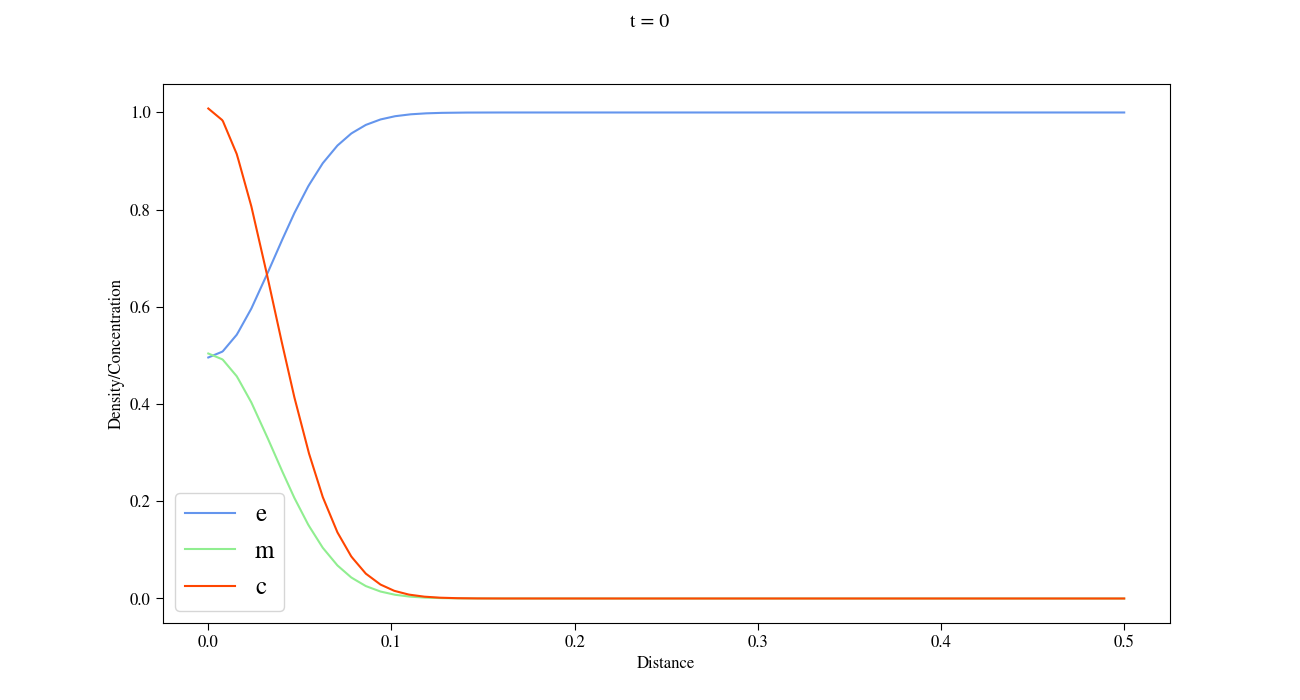
\includegraphics[width=\textwidth]{resources/images/inital_value_plot_figure.png}
    \caption{Visualization of the initial value distribution for an experiment in two space dimensions, radially symmetrical}
    \label{fig:Initial_Value_Distribution}
\end{figure}

For each of the modified free parameters $d_c, \gamma, \eta, d_m, \alpha, \beta, \mu_1, \mu_2$ we are going to take look at values or ranges which were used in previous experiments: 
\begin{itemize}
    \item $d_c = 0.001$
    \item $\gamma \in \{0.001, 0.002, 0.005\}$
    \item $\mu_1 \in \{0.1, 0.5\}$
    \item $\eta \in \{10, 20\}$
    \item $\mu_2 \in \{0.1, 0.5\}$
    \item $d_m \in \{0.001, 0.01\}$
    \item $\alpha \in \{0.1, 10\}$
    \item $\beta \in \{0, 0.07, 0.5\}$
\end{itemize}
Looking at these estimates leaves us with plenty of room to investigate the effects of every single non-fixed parameter. Since according to previous experiments this work will use the baseline set of parameters with $(d_c, \gamma, \mu_1, \eta, \mu_2, d_m, \alpha, \beta) = (0.001, 0.005, 0, 10, 0, 0.001,0.1, 0)$ for experiments without proliferation and 
$(d_c, \gamma, \mu_1, \eta, \mu_2, d_m, \alpha, \beta) = (0.001, 0.005, 0.3, 10, 0.3, 0.001,0.1, 0.1)$ for experiments with proliferation.







\begin{comment}
For each of the above parameters we are going to look reasonable ranges in which they are definded:
\begin{itemize}
    \item $D_c$: As explained it is cruical for tumor cells to have a high motility, evading the defense mechanisms of cells and invading surrouding tissue effectively. 
    The diffusion coefficient $D_c$ ranges with values ranging from ... to ...
    \item $D_m$: Since an extracellular matrix describes a network of extracellular macromolecules and minerals, it's diffusion properties heavily depend 
    on the components this network is build of, they can be for example be collagens or enzymes that provide structural and 
    biochemical support for the surrouding cells. This causes the coefficient to vary widely with a range of ... to .....
    \item $\chi$: The parameter $\chi$ describes movement responses of tumor cells to changes in attracting molecules concentration, like in our case the 
    extracellular matrix concentration. The parameter's range lies between ... and ....
    \item $\delta$: $\delta$ models the annihilation process of matrix-degrading enzymes and extracellular matrix macromolecules.
    It has usually a value between .. and ..
    \item $\mu_i$: The value of $\mu_i$ will respectively describe the production rate of tumor cells, extracellular matrix macromolecules and matrix-degrading enzymes, for $i\in \{1,2,3\}$.
    
    \item $\lambda$: This parameter describes the production rate of the matrix-degrading enzymes. Here we have values within the range ... to ...
\end{itemize}
These ranges will later govern the parameter analysis in the Experiment section.

\subsubsection{Diffusion Koefficient $D_x$}
Those parameters are now given an in-depth biological meaning and assumptions on their areas of definition. \newline 
Starting with $D_c$ and $D_m$, they are the diffusion coefficients, describing how fast a particle may diffuse through a medium. 
Diffusion means particles moving from areas of higher concentration to areas of lower concentration, with the goal of creating an equillibrium 
state, where everywhere of the defined space we have the same concentration of particles. For example knwoing from the biological foundation 
that cancer cells need to have a higher motility than normal cells to invade the surrouding tissue, the diffusion coefficients for 
the malignant cells is likely to be higher than the one of normal cells. 
In mathematical terms Fick's Law is often used to describe diffusion, creating a relationship between a concentration gradient and the flux of a substance. 
The flux describes the amount of a substances which crosses a unit area in unit time:
\begin{align}
    F = - D \frac{\partial c}{\partial x} = -D \nabla c
\end{align}
With this formulation 

\subsubsection{Haptotatic Flux Koefficient}
$\chi$

\subsubsection{Production and Decay Rates}
$\lambda$, $mu$


\subsubsection{Degradation}
$\delta$

\subsubsection{Assumptions}
\end{comment}
%\externaldocument{modelling}

\section{Method}

%correct systematic variation table

This work will investigate how the free parameters of the model given by the equations~\ref{eq:6} -~\ref{eq:10} will affect the spatial temporal progress of the numerical simulation. For the numerical simulation we will use the weak form given with equations~\ref{eq:11} -~\ref{eq:13} and solve it using HiFlow. To study the results of the numerical simulation ParaView is used, producing informative plots to compare the evolution of the simulation in time. For this we rely on the tool Plot Over Line to give radially symmetrical reulsts of the three variables of tumour and extracellular matrix density and matrix-degrading enzymes, like seen in the inital distribution in figure~\ref{fig:Initial_Value_Distribution}, in figure you can see the configuraion for the Plot Over Line tool used, the grey line in the middle of the simulation to the middle of the top of the square.\newline
\begin{figure}
    \centering
    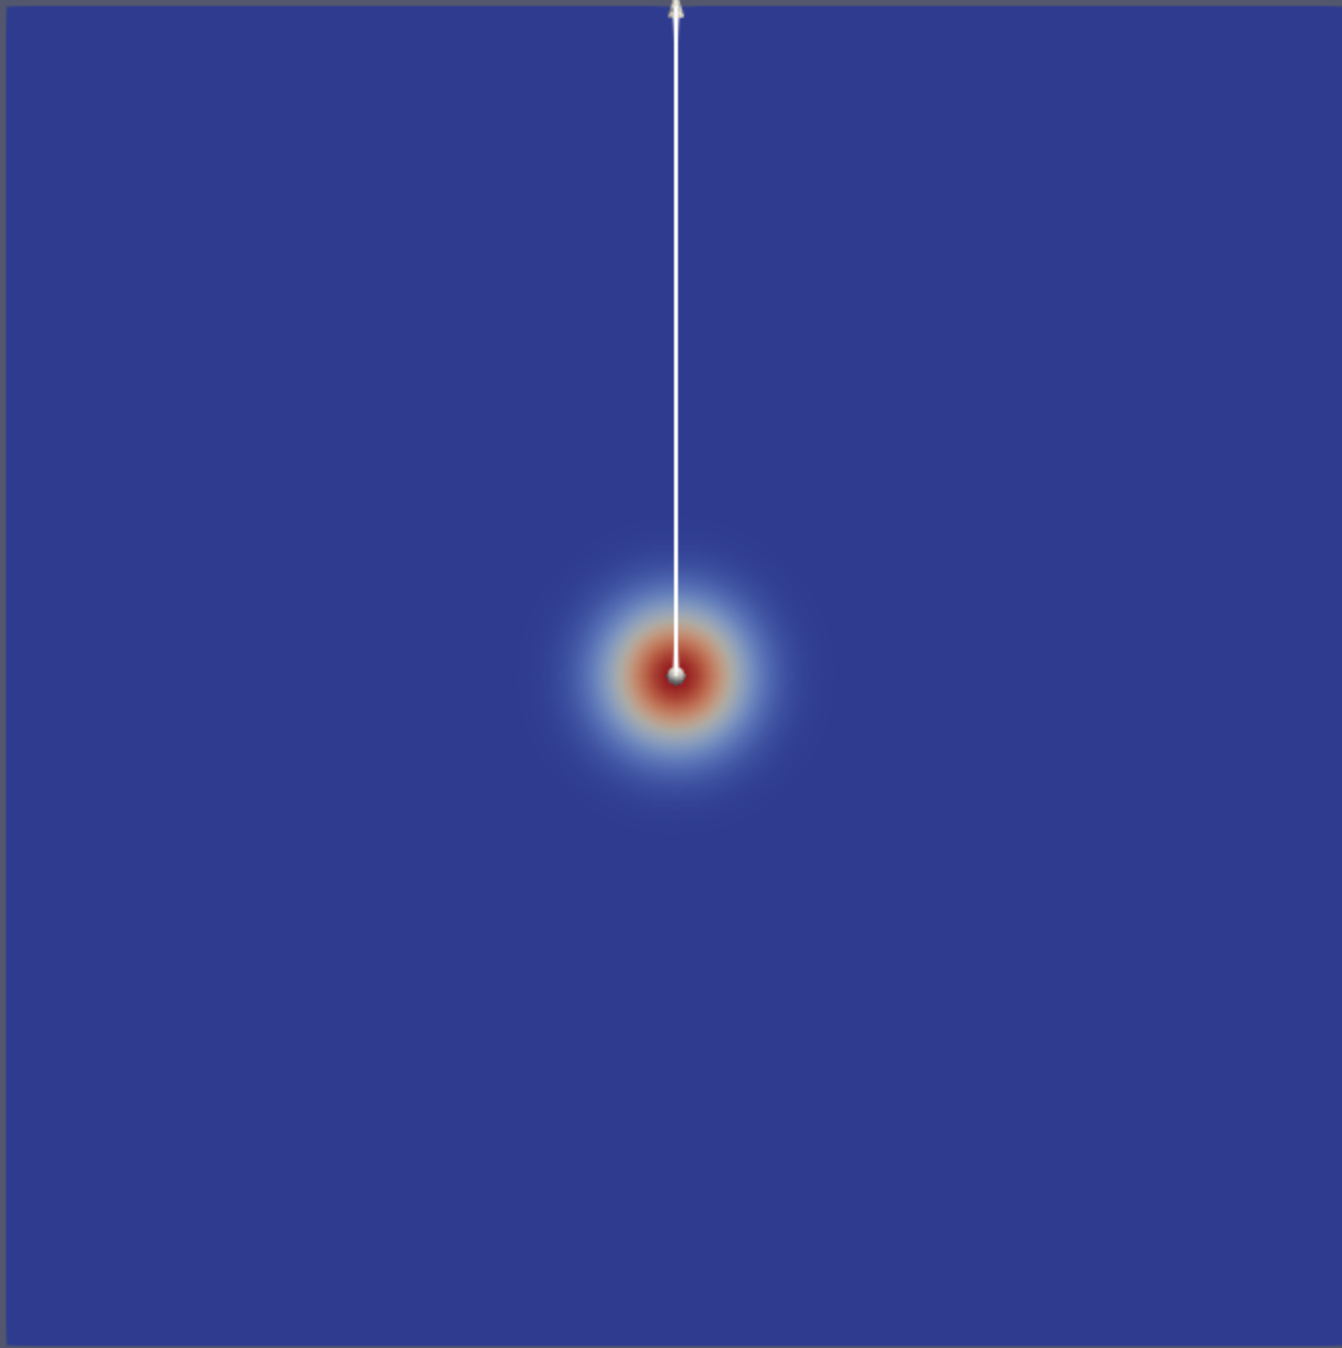
\includegraphics[width=0.3\textwidth]{resources/images/plot_over_line_tool.png}
    \caption{Plot Over Line Tool Configuration}
    \label{fig:PlotOverLine}
\end{figure}
All experiments, except when introducing the heterogenous ECM, start with the same initial values as seen in figuer initial values.\newline 
First replications of simulations of previous works will be discussed whhich serves the purpose to first verify the correctness of our result, as well as to give a starting point describing the phenomena this model exhibits. We start with the 2D case, since for this there are many examples already given and then move on to 3D simulation where the examples are fewer. \newline
After having taken a look at the preexisting experiments the main part of this work will begin with a systematic parameter analysis. Like before it will start investigating 2D simulation and will then move on to 3D simulation. Here we will also compare what effect the dimensionality has on the simulation, for example of the amount of overall values for $c,e,m$ and try replicating the behaviour of the 2D cases in the 3D variant. \newline
At last we will have a prospect on how an heterogneous extracellular matrix influences the results, which is the more realistic case, since tumourous cells tend to appear at border regions of tissue where we do not have a homogenous ECM, like it is rather found inside a tissue region. \newline
The results of the above experiments will be summarized and discussed in the Conclusion and Discussion part, pointing out the important characteristics of the simulation and disucssing the sensitivity of each of the parameters. At this point we will have an outlook on how to extend the model in more continuous and or discrete adaptations.
Looking at these estimates of section 3 we are left with plenty of room to investigate the effects of every single parameter. For this systematic analysis we are going to assume a baseline set of parameters, $(d_c, \gamma, \mu_1, \eta, \mu_2, d_m, \alpha, \beta) = (0.001, 0.005, 0, 10, 0, 0.001,0.1, 0)$ for experiments without proliferation and \newline
$(d_c, \gamma, \mu_1, \eta, \mu_2, d_m, \alpha, \beta) = (0.001, 0.005, 0.3, 10, 0.3, 0.001,0.1, 0.1)$ for experiments with proliferation, where in every experiment one paramter will be changed. Later this will be extended to study a cross-analysis, where more than one parameter is changed at a time. The set of baseline parameters is taken from previous experiments done by Anderson et al.~\cite{anderson_mathematical_2000} and Kolev et al.~\cite{Kolev2010}. The systematic variations will be same for 2D as well as 3D experiments and can be found in talbe~\ref{tab:systematic_analysis}.

\begin{table}[!h]
    \begin{center}
        \label{tab:systematic_analysis}
        \begin{tabular}{||c c c c||} 
            \hline
            Col1 & Col2 & Col2 & Col3 \\ [0.5ex] 
            \hline\hline
            1 & 6 & 87837 & 787 \\ 
            \hline
            2 & 7 & 78 & 5415 \\
            \hline
            3 & 545 & 778 & 7507 \\
            \hline
            4 & 545 & 18744 & 7560 \\
            \hline
            5 & 88 & 788 & 6344 \\ [1ex] 
            \hline
        \end{tabular}
        \caption{Your caption.}
    \end{center}
\end{table}

\begin{comment}

\subsection{Software and Implementation}
\subsection{Systematic Parameter Analysis}
\subsubsection{2D}
\subsubsection{3D}
\subsubsection{Non-heterogenous ECM Structure}

This work will investigate how the results of the modified model in the modelling section will be affected be varying free parameters $\lambda, \delta, \mu_1, \mu_2, \mu_3$ as well as how the chosen dimension for a simulation will influence the output.
For this we will start with comparing results first within the same dimension, varying the free parameters. Conducting these experiments we hope that we can see a pattern occuring, which is shared across one dimension. After this we will investigate how the results are changed when we change the dimension but keep the free parameters the same. 


\begin{center}
\begin{tabular}{|| c | c | c | c | c || c | c | c | c | c || c | c | c | c | c ||}
    \hhline{||=|=|=|=|=||=|=|=|=|=||=|=|=|=|=||}
    1D \small & & & & & 2D & & & & & 3D & & & & \\
    \hhline{||=|=|=|=|=||=|=|=|=|=||=|=|=|=|=||}
    $\lambda$ & $\delta$ & $\mu_1$ & $\mu_2$ & $\mu_3$  & $\lambda$ & $\delta$ & $\mu_1$ & $\mu_2$ & $\mu_3$ & $\lambda$ & $\delta$ & $\mu_1$ & $\mu_2$ & $\mu_3$ \\ 
    \hline
    a & b & c & d & e & a & b & c & d & e & a & b & c & d & e \\ \hline 
    a & b & c & d & e & a & b & c & d & e & a & b & c & d & e \\ \hline 
    a & b & c & d & e & a & b & c & d & e & a & b & c & d & e \\ \hline 
    a & b & c & d & e & a & b & c & d & e & a & b & c & d & e \\ \hhline{||=|=|=|=|=||=|=|=|=|=||=|=|=|=|=||} 

\end{tabular}
\end{center}

When comparing the effects of the free parameters on the simulation we need to keep in mind, that some of them are by assupmtion fixed, whilst others are defined within a reasonable range and again others have no restrictions at all, for those we assume the value ranges in the modelling section. At this first stage of the investigation we change only one parameter within each group of experiments, for example we only study how the output changes when $\delta$ changes, we do this with every parameter and compare the results within their dimension. When we are done with that we compare the results with changing dimension whilst keeping every other free parameter equal. \newline
With the core question that if different dimensions yield different results, we hope to find characteristics prevailing in each dimension, but mainly concentrate on the features that arise with the same choice of parameters varying the dimension. We hope to find answers to which changes in outcome emerge and how to explain the different results. \newline
As a last step this work compares the found results with clinical results, from in-vitro results. Why in-vitro, because this models lacks the biological complexity which governs many effects regarding tumor growth in living bodies, which would yield to quite different behaviour.
\end{comment}
\externaldocument{modelling}

\section{Experiments and Results}
\label{sec:experiments}

All experiments that consider the ECM to be homogenous start with the same initial values as seen in figure~\ref{fig:2D_homogenous_ECM_initial}. Experiments observing the effects of a heterogenous ECM use different initial values, as seen in figure~\ref{fig:2D_heterogenous_ECM_initial}.\newline 
Solving the numerical model HiFlow\textsuperscript{3} will be used with the weak form given with equations~\ref{eq:11} -~\ref{eq:13}. To evaluate the results of the numerical simulation ParaView~\cite{paraview} is used, producing informative plots to compare the evolution of the simulation in time. For this we rely on the tool Plot Over Line to give results for the three variables of tumor cell density, extracellular matrix density and matrix-degrading enzymes concentration. This tool also allows us to compare all three variables in one plot whereas using 2D plots we would need to have one for each variable. Using it makes the results better readable and allows a clearer quantitative insight into the experiments as you will see in figure~\ref{fig:unadjsuted_replication}.\newline
This work starts with replicating numerical simulations done by other papers in higher dimensions. Since there were only 1D simulations done previously, the model will be adjusted in such a way, that the Plot Over Line graphs mimick the plots given by the previous experiments. This will serve two purposes, first it will verify a correct implementation of the model and second this will give us a starting point by which we can vary the parameters, investigating the phenomena this model exhibits. \newline 
We will start with examining 2D experiments with homogenous ECMs, using our model with the parameters $\mu_1$ and $\mu_2$ both set to zero, considering a case with no proliferation of tumor cells and no renewal of the extracellular matrix molecules, after this we will introduce proliferation and renewal, Incorporating $\mu_1$ and $\mu_2$ into the variation.
Considering 3D experiments we will do a slimmer replication and parameter analysis due to the immense computational effort. After examining the model with a homogenous ECM initial condition we will move on to look at a case considering a heterogenous ECM in 2D.\newline
Looking at the parameter estimates from \cite{anderson_mathematical_2000} to non-dimensionalise the time, we see that with $L \in [0.1cm,1cm]$ and $D\approx 10^{-6}\frac{cm^2}{s}$, $\tau = \frac{L^2}{D}$ would give us a big temporal range, $\tau_{min} = 1000s$ and $\tau_{max} = 1000000s$ in which the simulations take place. However using estimates taken from~\cite{STEPHANOU200696} and~\cite{franssen_mathematical_2019} for the length scale, with $L=0.2cm$ gives us a concrete value for our non-dimensional time, $\tau=40000s$, from now on $t$ will stand as replacement for $\tau$ for simplicity reason.\newline 
Since Anderson et al. don't specify their exact value used for $L$, we needed to determine appropriate configurations for $dt$ used in our simulation to get comparable results. We used a timestep of $dt=0.01$ which corresponds to $400s$ and let the simulations run for a dimensionless time of $t=8$ corresponding to $320000s=88$ $days$. Looking at the results below we found that for every unit of time in Anderson et al's experiments, in our experiements $t=0.4$ have passed.\newline 
Another challenge are the diffusion coefficients, since they are dependent on the dimension we are in, we have to find our own estimates as a baseline value. \newline 
For each stage of experiments we will use a set of baseline parameters, which will be evaluated experimentally, and from there vary one or more parameter at a time to get an overview of their effects. \newline
For all the plots of the experiments the red curve indicates the tumor cell density, the blue curve the ECM density and the green curve the MDE concentration. In all of the experiments we used the value of $\epsilon = 0.01$ to match the inital conditions from \cite{anderson_mathematical_2000} and \cite{Kolev2010}. \newline 

\subsection{Two dimensional Results without Proliferation and Renewal}
\label{sec:2D_without_proliferation}

We assume for the initial conditions that at dimensionless time $t=0$ there is already a nodule of cells located at the center of the unit domain $\Omega$ that has produced a concentration of matrix-degrading enzymes and has already degraded the extracellular matrix at the center. Furthermore we assume the extracellular matrix structure to be homogenous.\newline 
We define the initial conditions for the tumor cell denisity as:
\begin{align*}
    c(x,0)= \exp(\frac{-(x-0.5)^2}{0.01})
\end{align*}
The initial conditions of the matrix-degrading enzymes are describes as:
\begin{align*}
    m(x,0) = 0.5 c(x,0) = 0.5 \exp(\frac{-(x-0.5)^2}{0.01})
\end{align*}
The strucutre of the extracellular matrix looks as follow:
\begin{align*}
    e(x,0) = 1 - 0.5 c(x,0) = 1 - 0.5 \exp(\frac{-(x-0.5)^2}{0.01})
\end{align*}
\begin{figure}[h]
    \centering
    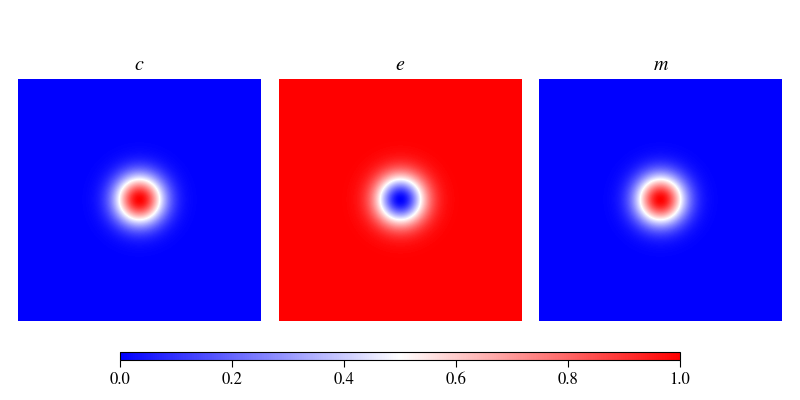
\includegraphics[width=\textwidth]{resources/images/2D_initial_conditions_homogenous_ECM.png}
    \caption{Visualization of the initial value distribution for an experiment in two space dimensions with a homogenous extracellular matrix}
    \label{fig:2D_homogenous_ECM_initial}
\end{figure}
Figure~\ref{fig:2D_homogenous_ECM_initial} shows a 2D plot of the initial conditions using the homogenous extracellular matrix structure. For all three images you see that at the center there is either a high concentration, tumor cell density and matrix degrading enzymes concentration or a low concentration, the extracellular matrix.\newline 

\begin{longtable}{|c c c c c c c c c c|}
    \hline
    Figure & Linestyle & $d_c$ & $\gamma$ & $\mu_1$ & $\eta$ & $\mu_2$ & $d_m$ & $\alpha$ & $\beta$ \\ [0.5ex] 
    \hline\hline
    \endfirsthead
    \hline
    Figure & Linestyle & $d_c$ & $\gamma$ & $\mu_1$ & $\eta$ & $\mu_2$ & $d_m$ & $\alpha$ & $\beta$ \\ [0.5ex] 
    \hline\hline
    \endhead
    \hline \multicolumn{10}{|r|}{{continued on next page}} \\ \hline
    \endfoot
    \endlastfoot
    \ref{fig:unadjsuted_replication} & \sampleline{} & $1\cdot 10^{-3}$ & $0.005$ & $0$ & $10$ & $0$ & $1\cdot 10^{-3}$ & $0.1$ & $0$\\  \hline
    \ref{fig:replication_alpha_comparison} & \sampleline{dash pattern=on .7em off .2em on .05em off .2em} & $1\cdot 10^{-3}$ & 0.005 & 0 & 10 & 0 & $1\cdot 10^{-3}$ & 0.2 & 0\\  \hline
    \ref{fig:replication_alpha_comparison} & \sampleline{dotted} & $1\cdot 10^{-3}$ & 0.005 & 0 & 10 & 0 & $1\cdot 10^{-3}$ & 0.3 & 0\\  \hline
    \ref{fig:replication_alpha_comparison} & \sampleline{} & $1\cdot 10^{-3}$ & 0.005 & 0 & 10 & 0 & $1\cdot 10^{-3}$ & 0.35 & 0\\  \hline
    \ref{fig:replication_alpha_comparison} & \sampleline{dashed} & $1\cdot 10^{-3}$ & 0.005 & 0 & 10 & 0 & $1\cdot 10^{-3}$ & 0.4 & 0\\  \hline
    \ref{fig:replication_dc_comparison} & \sampleline{dash pattern=on .7em off .2em on .05em off .2em} & $1\cdot 10^{-3}$ & 0.005 & 0 & 10 & 0 & $1\cdot 10^{-3}$ & 0.3546 & 0\\  \hline
    \ref{fig:replication_dc_comparison} & \sampleline{dotted} & $1\cdot 10^{-4}$ & 0.005 & 0 & 10 & 0 & $1\cdot 10^{-3}$ & 0.3546 & 0\\  \hline
    \ref{fig:replication_dc_comparison} & \sampleline{} & $5\cdot 10^{-4}$ & 0.005 & 0 & 10 & 0 & $1\cdot 10^{-3}$ & 0.3546 & 0\\  \hline
    \ref{fig:replication_dc_comparison} & \sampleline{dashed} & $1\cdot 10^{-5}$ & 0.005 & 0 & 10 & 0 & $1\cdot 10^{-3}$ & 0.3546 & 0\\  \hline
    \ref{fig:replication_gamma_comparison} & \sampleline{dash pattern=on .7em off .2em on .05em off .2em} & $5\cdot 10^{-5}$ & 0.005 & 0 & 10 & 0 & $1\cdot 10^{-3}$ & 0.3546 & 0\\  \hline
    \ref{fig:replication_gamma_comparison} & \sampleline{dotted} & $5\cdot 10^{-4}$ & 0.0055 & 0 & 10 & 0 & $1\cdot 10^{-3}$ & 0.3546 & 0\\  \hline
    \ref{fig:replication_gamma_comparison} & \sampleline{} & $5\cdot 10^{-4}$ & 0.006 & 0 & 10 & 0 & $1\cdot 10^{-3}$ & 0.3546 & 0\\  \hline
    \ref{fig:replication_gamma_comparison} & \sampleline{dashed} & $5\cdot 10^{-4}$ & 0.007 & 0 & 10 & 0 & $1\cdot 10^{-3}$ & 0.3546 & 0\\  \hline
    \ref{fig:basecase_without_proliferation} & \sampleline{} & $5\cdot 10^{-4}$ & 0.0055 & 0 & 10 & 0 & $1\cdot 10^{-3}$ & 0.3546 & 0\\ \hline
    \ref{fig:dc_variation} & \sampleline{dash pattern=on .7em off .2em on .05em off .2em} & $5\cdot 10^{-5}$ & 0.0055 & 0 & 10 & 0 & $1\cdot 10^{-3}$ & 0.3546 & 0\\ \hline
    \ref{fig:dc_variation} & \sampleline{} & $1\cdot 10^{-4}$ & 0.0055 & 0 & 10 & 0 & $1\cdot 10^{-3}$ & 0.3546 & 0\\ \hline
    \ref{fig:dc_variation} & \sampleline{dotted} & $1\cdot 10^{-3}$ & 0.0055 & 0 & 10 & 0 & $1\cdot 10^{-3}$ & 0.3546 & 0\\ \hline
    \ref{fig:gamma_variation} & \sampleline{dotted} & $5\cdot 10^{-4}$ & 0.002 & 0 & 10 & 0 & $1\cdot 10^{-3}$ & 0.3546 & 0\\ \hline
    \ref{fig:gamma_variation} & \sampleline{} & $5\cdot 10^{-4}$ & 0.008 & 0 & 10 & 0 & $1\cdot 10^{-3}$ & 0.3546 & 0\\ \hline
    \ref{fig:gamma_variation} & \sampleline{dashed} & $5\cdot 10^{-4}$ & 0.01 & 0 & 10 & 0 & $1\cdot 10^{-3}$ & 0.3546 & 0\\ \hline
    \ref{fig:gamma_2D_plot} & \sampleline{} & $5\cdot 10^{-4}$ & 0.1 & 0 & 10 & 0 & $1\cdot 10^{-3}$ & 0.3546 & 0\\ \hline
    \ref{fig:gamma_pol_comparison} & \sampleline{} & $5\cdot 10^{-4}$ & 0.1 & 0 & 10 & 0 & $1\cdot 10^{-3}$ & 0.3546 & 0\\ \hline
    \ref{fig:eta_variation} & \sampleline{dotted} & $5\cdot 10^{-4}$ & 0.0055 & 0 & 2 & 0 & $1\cdot 10^{-3}$ & 0.3546 & 0\\ \hline
    \ref{fig:eta_variation} & \sampleline{} & $5\cdot 10^{-4}$ & 0.0055 & 0 & 12 & 0 & $1\cdot 10^{-3}$ & 0.3546 & 0 \\ \hline
    \ref{fig:eta_variation} & \sampleline{dotted} & $5\cdot 10^{-4}$ & 0.0055 & 0 & 20 & 0 & $1\cdot 10^{-3}$ & 0.3546 & 0 \\ \hline
    \ref{fig:dm_variation} & \sampleline{dotted} & $1\cdot 10^{-3}$ & 0.0055 & 0 & 10 & 0 & 0.00001 & 0.3546 & 0 \\ \hline
    \ref{fig:dm_variation} & \sampleline{} & $1\cdot 10^{-4}$ & 0.0055 & 0 & 10 & 0 & 0.001 & 0.3546 & 0 \\ \hline
    \ref{fig:dm_variation} & \sampleline{dashed} & $1\cdot 10^{-5}$ & 0.0055 & 0 & 10 & 0 & 0.1 & 0.3546 & 0 \\ \hline
    \ref{fig:alpha_variation} & \sampleline{dotted} & $5\cdot 10^{-4}$ & 0.0055 & 0 & 10 & 0 & $1\cdot 10^{-3}$ & 0 & 0 \\ \hline
    \ref{fig:alpha_variation} & \sampleline{} & $5\cdot 10^{-4}$ & 0.0055 & 0 & 10 & 0 & $1\cdot 10^{-3}$ & 0.6 & 0 \\ \hline
    \ref{fig:alpha_variation} & \sampleline{dotted} & $5\cdot 10^{-4}$ & 0.0055 & 0 & 10 & 0 & $1\cdot 10^{-3}$ & 1.0 & 0 \\ \hline
    \ref{fig:beta_variation} & \sampleline{dotted} & $5\cdot 10^{-4}$ & 0.0055 & 0 & 10 & 0 & $1\cdot 10^{-3}$ & 0.3546 & 0.1 \\ \hline
    \ref{fig:beta_variation} & \sampleline{} & $5\cdot 10^{-4}$ & 0.0055 & 0 & 10 & 0 & $1\cdot 10^{-3}$ & 0.3546 & 0.01 \\ \hline
    \ref{fig:beta_variation} & \sampleline{dotted} & $5\cdot 10^{-4}$ & 0.0055 & 0 & 10 & 0 & $1\cdot 10^{-3}$ & 0.3546 & 0.005 \\ \hline
    \ref{fig:dc_gamma_variation} - left& \sampleline{dotted} & $5\cdot 10^{-5}$ & 0.001 & 0 & 10 & 0  & $1\cdot 10^{-3}$ & 0.3546 & 0 \\ \hline
    \ref{fig:dc_gamma_variation} - left & \sampleline{} & $5\cdot 10^{-5}$ & 0.01 & 0 & 10 & 0 & $1\cdot 10^{-3}$ & 0.3546 & 0 \\ \hline
    \ref{fig:dc_gamma_variation} -right & \sampleline{dotted} & $1\cdot 10^{-3}$ & 0.001 & 0 & 10 & 0 & $1\cdot 10^{-3}$ & 0.3546 & 0 \\ \hline
    \ref{fig:dc_gamma_variation} -right & \sampleline{} & $1\cdot 10^{-3}$ & 0.01 & 0 & 10 & 0 & $1\cdot 10^{-3}$ & 0.3546 & 0 \\ \hline
    \ref{fig:dm_eta_variation} - left & \sampleline{dotted} & $5\cdot 10^{-4}$ & 0.0055 & 0 & 2 & 0 & $1\cdot 10^{-5}$ & 0.3546 & 0 \\ \hline
    \ref{fig:dm_eta_variation} - left & \sampleline{} & $5\cdot 10^{-4}$ & 0.0055 & 0 & 20 & 0 & $1\cdot 10^{-5}$ & 0.3546 & 0 \\ \hline
    \ref{fig:dm_eta_variation} -right & \sampleline{dotted} & $5\cdot 10^{-4}$ & 0.0055 & 0 & 2 & 0 & $1\cdot 10^{-3}$ & 0.3546 & 0 \\ \hline
    \ref{fig:dm_eta_variation} -right & \sampleline{} & $5\cdot 10^{-4}$ & 0.0055 & 0 & 20 & 0 & $1\cdot 10^{-3}$ & 0.3546 & 0 \\ \hline
    \ref{fig:alpha_beta_variation} - left & \sampleline{dotted} & $5\cdot 10^{-4}$ & 0.0055 & 0 & 10 & 0 & $1\cdot 10^{-3}$ & 0.1 & 0.005 \\ \hline
    \ref{fig:alpha_beta_variation} - left & \sampleline{} & $5\cdot 10^{-4}$ & 0.0055 & 0 & 10 & 0 & $1\cdot 10^{-3}$ & 0.1 & 0.1 \\ \hline
    \ref{fig:alpha_beta_variation} -right & \sampleline{dotted} & $5\cdot 10^{-4}$ & 0.0055 & 0 & 10 & 0 & $1\cdot 10^{-3}$ & 1.0 & 0.005 \\ \hline
    \ref{fig:alpha_beta_variation} -right & \sampleline{} & $5\cdot 10^{-4}$ & 0.0055 & 0 & 10 & 0 & $1\cdot 10^{-3}$ & 1.0 & 0.1 \\ \hline
    \ref{fig:dm_alpha_beta_variation_1} - left & \sampleline{dotted} & $5\cdot 10^{-4}$ & 0.0055 & 0 & 10 & 0 & $1\cdot 10^{-5}$ & 0.1 & 0.005 \\ \hline
    \ref{fig:dm_alpha_beta_variation_1} - left & \sampleline{} & $5\cdot 10^{-4}$ & 0.0055 & 0 & 10 & 0 & $1\cdot 10^{-5}$ & 0.1 & 0.1 \\ \hline
    \ref{fig:dm_alpha_beta_variation_1} -right & \sampleline{dotted} & $5\cdot 10^{-4}$ & 0.0055 & 0 & 10 & 0 & $1\cdot 10^{-5}$ & 1.0 & 0.005 \\ \hline
    \ref{fig:dm_alpha_beta_variation_1} -right & \sampleline{} & $5\cdot 10^{-4}$ & 0.0055 & 0 & 10 & 0 & $1\cdot 10^{-5}$ & 1.0 & 0.1 \\ \hline
    \ref{fig:dm_alpha_beta_variation_2} - left & \sampleline{dotted} & $5\cdot 10^{-4}$ & 0.0055 & 0 & 10 & 0 & $1\cdot 10^{-3}$ & 0.1 & 0.005 \\ \hline
    \ref{fig:dm_alpha_beta_variation_2} - left & \sampleline{} & $5\cdot 10^{-4}$ & 0.0055 & 0 & 10 & 0 & $1\cdot 10^{-3}$ & 0.1 & 0.1 \\ \hline
    \ref{fig:dm_alpha_beta_variation_2} -right & \sampleline{dotted} & $5\cdot 10^{-4}$ & 0.0055 & 0 & 10 & 0 & $1\cdot 10^{-3}$ & 1.0 & 0.005 \\ \hline
    \ref{fig:dm_alpha_beta_variation_2} -right & \sampleline{} & $5\cdot 10^{-4}$ & 0.0055 & 0 & 10 & 0 & $1\cdot 10^{-3}$ & 1.0 & 0.1 \\ \hline
    \caption{Overview of all experiments conducted for the model without proliferation and renewal producing 2D output}
    \label{table:2D_experiments_without_proliferation}
\end{longtable}
Table~\ref{table:2D_experiments_without_proliferation} shows all the experiments done in two space dimensions using the model without proliferation or renewal. You can see the figure and the linestyle to verify exactly which experiment uses which values. 
    
\subsubsection{Replicating results}
We will start with replicating the first experiment from  Anderson et al.\cite{anderson_mathematical_2000}.  Figure~\ref{fig:anderson_experiment} shows a screenshot of this experiment, unfortunately in low resolution, since the original paper had not included any digital data containing the diagrams of their results.
\begin{figure}[h!]
    \centering
    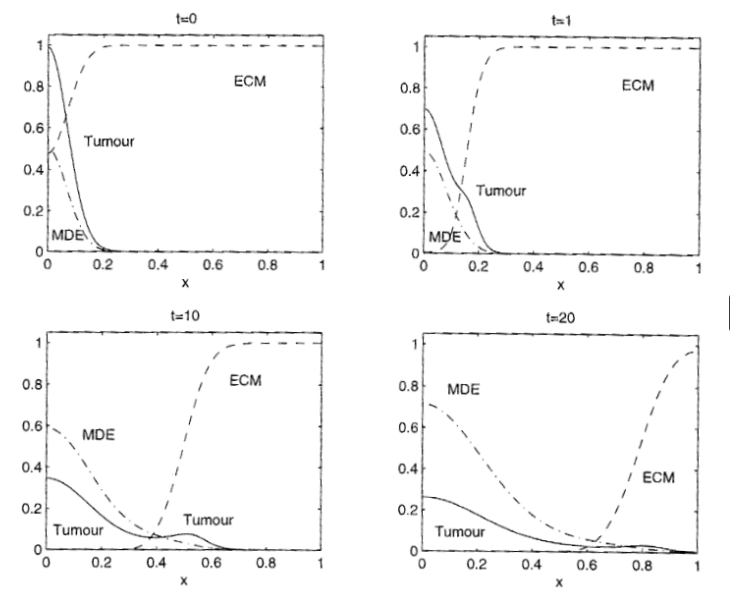
\includegraphics[width=0.85\textwidth]{resources/images/anderson_experiment.png}
    \caption{Andersons first one dimensional experiment using the parameter values $d_c = 1\cdot 10^{-3}, d_m = 1\cdot 10^{-3}, \gamma = 0.005, \eta = 10, \alpha = 0.1, \beta = 0, \mu_1 = 0, \mu_2 = 0$}
    \label{fig:anderson_experiment}
\end{figure}
In figure~\ref{fig:anderson_experiment} you can see that after $t=1$ in their timescale the tumor cells start to develop a secession at the part invading the tissue. This secession propagates to a pointy peak in the later point in time. The concentration of the matrix-degrading enzymes increases continuously and the concentration of the extracellular matrix decreases continuously. We see that their $x$-axis is streched or rescaled to show an intervale from $0$ to $1$. In our case the interval on the plots has only $x$-values from $0$ to $0.5$.
\begin{figure}[ht!]
    \centering
    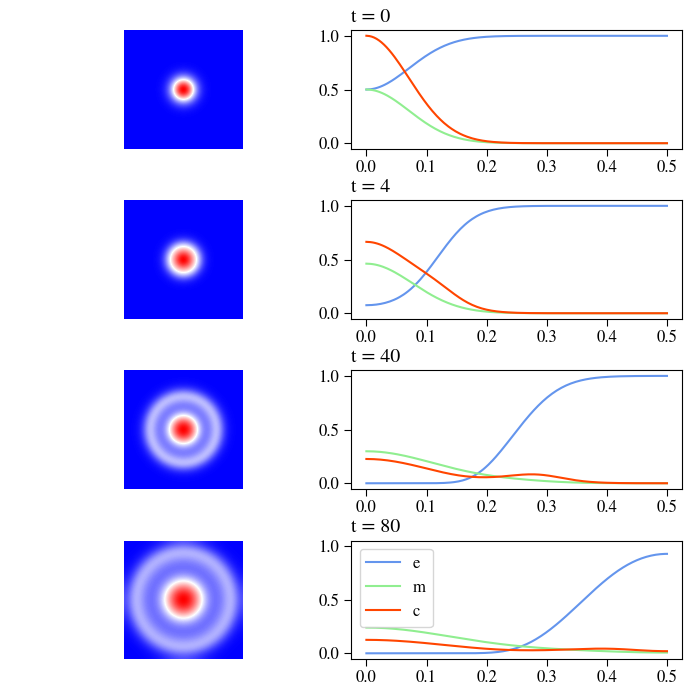
\includegraphics[width=0.85\textwidth]{resources/images/first_replication_results.png}
    \caption{Results using Anderson et al's parameters, left side 2D tumor cell density plots, right side results produced by applying the Plot Over Line tool}
    \label{fig:unadjsuted_replication}
\end{figure}
Replicating this experiment in two dimensions we start with the same parameters as Anderson et al. had used, $d_c = 1\cdot 10^{-3}, d_m = 1\cdot 10^{-3}, \gamma = 0.005, \eta = 10, \alpha = 0.1, \beta = 0$. Figure~\ref{fig:unadjsuted_replication} shows these results for four different points in time. On the left side you can see the two dimensional plots of the tumor cell density and on the right side you can see plots produced by applying the Plot Over Line tool. As mentioned above we will, for the most part, resort to using only the results produced by the Plot Over Line tool. You can see in the plots of figure~\ref{fig:unadjsuted_replication} on the right side the curves for the three variables are clearly distinguishable and we can estimate their values spacially and temporarily better, than using 2D plots to estimate values.\newline
Starting from the inital values we see that after $t=4$ a very small secession of the tumor cells is starting to form. This secession 
increases in the image at $t=4$, but at $t=8$ it has visibly flattened. This secession is not as pointy as seen in the one dimensional experiments. The interplay of the diffusion and haptotaxis factors determine how big this secession will be that splits from the main lump of the tumor cells and invades the tissue at a faster rate. It will also decide how pointy this secondary lump of tumor cells will be. Biologically this realtion between diffusion and haptotaxis translates to the invasion pace of the tumor cells and the rate of how much of them will remain at the center and how much will invade farther out into the tissue.\newline 
Looking at the concentration for the matrix degrading enzymes we see that it is here visily lower than in Anderson et al's experiement. We see little increase across time. This is due to the production factor of $\alpha$. This factor determines how fast the tumor cells produce the matrix-degrading enzymes that are degrading the extracellular matrix and allow the tumor cells to invade the tissue further.\newline 
Only the extracellular matrix concentration seems to mimick the behaviour of Anderson et al's experiment. It decreases continuously and in the last image you can see there is still a considerable amount left.\newline 
To replicate Anderson et al's results we will start adjusting the mentioned parameters of diffusion coefficient of the tumor cells, haptotatic coeff of the tumor cells and the production rate of the matrix-degrading enzymes. Making the curves fit prefectly will be impossible due to the high degrees of freedom of the system and the change of dimension. Regradless we will replicate as best as possible with a special focus on the values the variables will take at the origin $x=0$.\newline 
\begin{figure}[!htb]
    \centering
    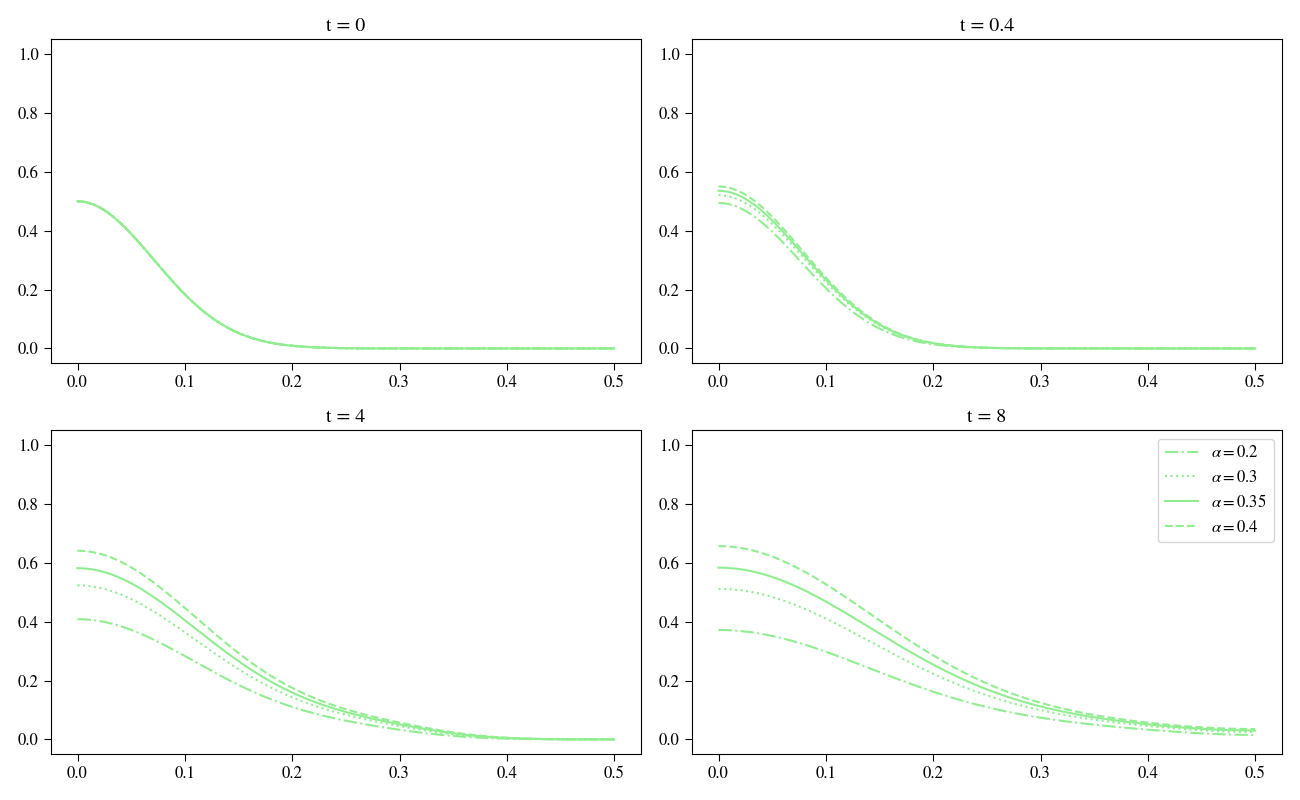
\includegraphics[width=\textwidth]{resources/images/alpha_comparison.png}
    \caption{Comparison of $\alpha$ values to replicate Anderson et al's experiment}
    \label{fig:replication_alpha_comparison}
\end{figure}
Starting with comparing different values for $\alpha$, we see in figuer~\ref{fig:replication_alpha_comparison} a comparison of how this affects the curve for matrix-degrading enzyme concentration. A maximum difference between the compared values of $0.2$ already causes drastic changes as you can see. In Anderson et al's experiment we observe a value of approximately $m(0,1)=0.5$ after, in their timescale, $t=1$ at the origin. This is mimicked best in our case for a value of $\alpha=0.2$. Thoug in the later points in time we see that this value for $\alpha$ is insufficiently low in terms of increase, though choosing $\alpha$ higher than $\alpha=0.4$ results in a accellerated ECM degradation that is too fast. Taking a value between those two allowed our simulations to exhibit the observed behaviour. We choose a value of $\alpha=0.35645$ to use in the later experiments as a basecase.\newline
\begin{figure}[!htb]
    \centering
    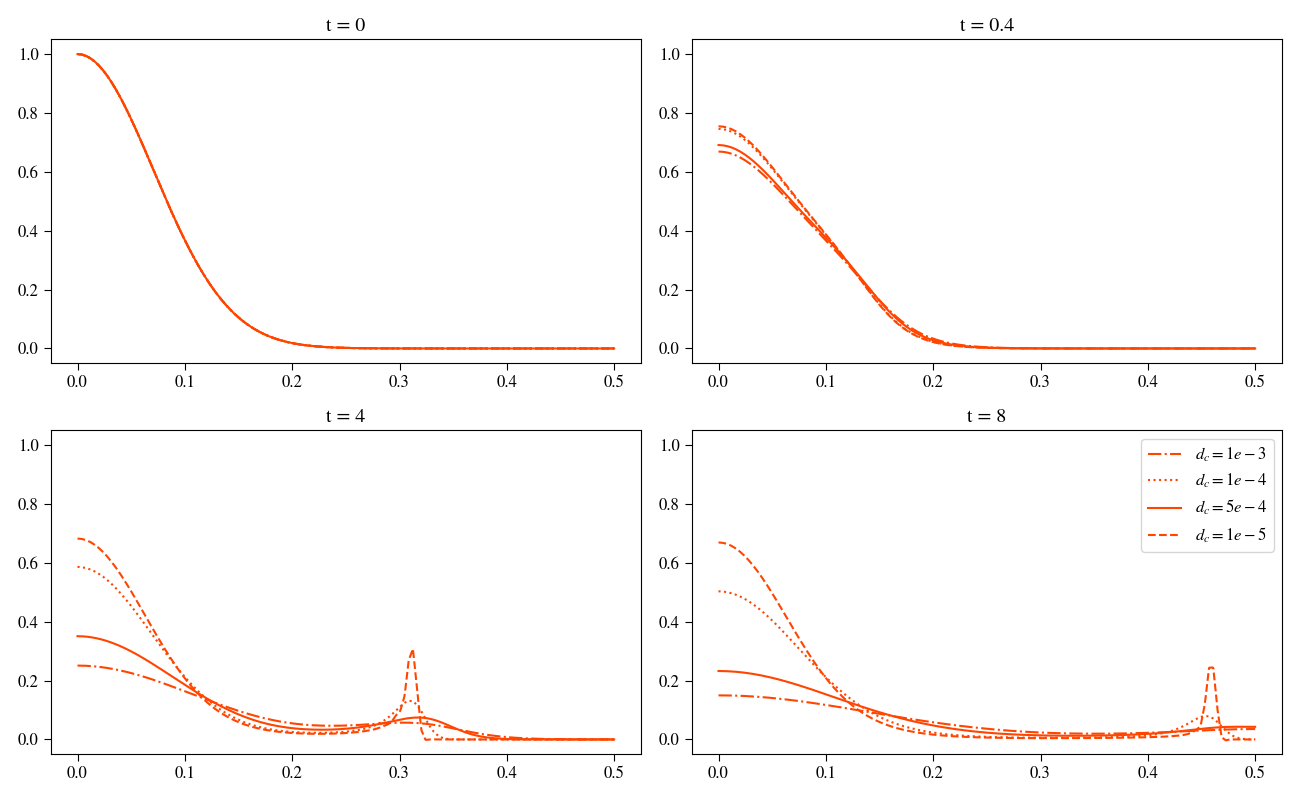
\includegraphics[width=\textwidth]{resources/images/dc_comparison.png}
    \caption{Comparison of $d_c$ values to replicate Anderson et al's experiment}
    \label{fig:replication_dc_comparison}
\end{figure}
Looking now at the diffusion coefficient for the tumor cells, in figure~\ref{fig:replication_dc_comparison} you can see different $d_c$ values compared in regard to the tumor cell concentration. It is clear that with decreasing $d_c$ the sharpness of the secondary lump of cells that forms to invade the tissue drastically increases due to increased effects of haptotaxis being now the main factor to control tumor motility, though we also observe that with decreasing $d_c$ the remaining lump of tumor cells at the origin also increases, due to little diffusion here. Over time we found that $dc=5 \cdot 10^{-4}$ describes Anderson et al's experimental results best for our simulations, with roughly matching density of tumor cells that remains at the origin at all times and, for our case, balanced effects of haptotaxis and diffusion.\newline
\begin{figure}[!htb]
    \centering
    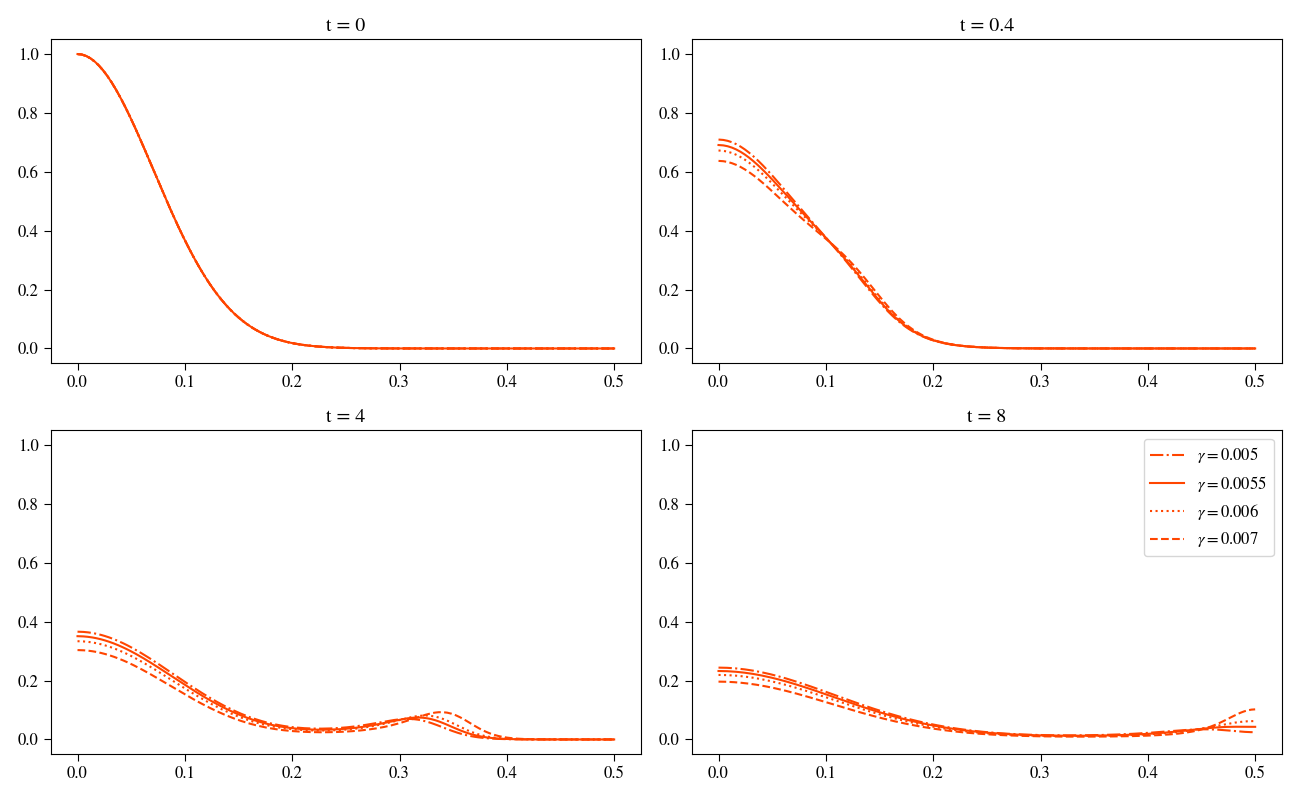
\includegraphics[width=\textwidth]{resources/images/gamma_comparison.png}
    \caption{Comparison of $\gamma$ values to replicate Anderson et al's experiment}
    \label{fig:replication_gamma_comparison}
\end{figure}
At last we want to adjust the haptotatic pull slightly, for this we are looking at a comparision of different $\gamma$ values in figure~\ref{fig:replication_gamma_comparison} depicting the tumor cell density. Comparing our results with Anderson et al's we want a larger secondary lump that invades the tumor cells faster than the one remaining at the origin. For this we need to increase $\gamma$ to increase the haptotaic pull that controls tumor cells motility. In the figure you see that incresing $\gamma$ yields these effects, but increasing it too much results in a too fast invasion pace of the surrounding tissue. Increasing $\gamma$ slightly to $\gamma=0.0055$ is already sufficient to produce the desried effects.\newline

\begin{comment}
Diffusion and Haptotaxis have stretched the curve for the tumor cells along the x-axis as did diffusion for the MDEs. The ECM has  been visibly degraded at the origin, being still fully present in outer regions exceeding $x\approx 0.2$.\newline
The next image shows the simulation after $0.4$ timesteps; we see that the secession of the tumor cell concentration of the previous point in time has been propagated to form a small hill at the leading edge of the tumor cells invading the surrounding tissue, this effect is due to the haptotatic influence, which pulls the tumor cells further into the accessible area towards higher values of $\nabla (c \nabla e)$, creating a seperation for the tumor cells, where the other part is still oriented towards the origin. The MDEs also continue their diffusion into the area, degrading the ECM in their wake.\newline 
In the last image, after 8 simulation time steps, we see that as well the hill that has formed at the leading edge of the tumor cells as well as the concentration of tumor cells at the origin, have flattened visibly and striving to take on a constant concentration throughout space, though we can still clearly distinguish both areas. If we were to look at the simulation at later points in time, the curve will flatten even more, since with more time the ECM will be further degraded and therefore the haptotactic flux coefficient $\gamma$ will lose its significance, leaving the movement of the tumor cells to diffusion only and spreading them constantly along the x-axis. The curve for the MDEs will also flattened due to diffusion,with the MDEs degrading the rest of the extracellular matrix molecules decrease their concentration further and the MDE concentration will increase over time due to no limiting factors in this experiment and on-going production contributed by the tumor cells $c$.\newline
Comparing \ref{fig:unadjsuted_replication} to figure 1 in \cite{anderson_mathematical_2000}, we can see major differences. The first image showing $t=0$ looks the same, which confirms that both experiments start with the same initial values condition. In the images showing the simulation at the second time checkpoint we see that though the tumor concentration and ECM density values are approximately the same, the MDE concentration is slightly lower in our experiment, which will get more pregnant in the later images. The unevenness having formed at the leading edge of the tumor cell concentration is also slightly smaller. The differences in the third image are more striking, both $c$ and $m$ have considerably lower concentrations, yet the ECM value looks is very similar. \newline 
In our case the diffusion and haptotatic pull of the tumor cells has shown to be too stong making the invasion process into the tissue happen too fast. The last time checkpoints strengthens our findings, showing the same behaviour with ECM being approximately the same, tumor cell density and MDE concentration being clearly lower in our experiment and invasion of tissue happening too fast, leaving the lump at the origin $x=0$ too small. \newline 
This first of all confirms the initial supposition that with changing the dimension for the simulations the results also vary. We will now adjust the parameters iteratively to make the results using two dimensions mimick the results from Anderson et. al as closely as possible. For this we will start with varying the MDE production coefficient $\alpha$, to get higher concentration values for the MDEs, and change the diffusion as well as haptotaxis coefficients of the tumor cells $d_c$ and  $\gamma$, to adjust the motitlity of the tumor cells and therefore also influence the invasion speed of them into the surrouding tissue.
Figures~\ref{fig:replication_alpha_comparison}, ~\ref{fig:replication_dc_comparison} and ~\ref{fig:replication_gamma_comparison} show these comparisons of the parameters $\alpha$, $d_c$ and $\gamma$. Comparing different values for $\alpha$ and their effect on the curve of the MDE concentration, shows in figure~\ref{fig:replication_alpha_comparison} that, especially looking at the later points in time $t=4$ and $t=8$, with values for $\alpha$ between $0.3$ and $0.4$ we will get a good approximation. The values of the original paper for the MDEs are for $t=4$ approximately $0.6$ at $x=0$ and for $t=8$ about $0.7$ at the same point in space. With a value  $\alpha=0.35645$ we got the best results regarding the MDE concentration.\newline 
Looking at $d_c$ we chose a value of $d_c=5\cdot 10^{-4}$. Using values below $0.00001$ will result in numerical instabilities and results that are not longer useable. For $\gamma$ we made a slight adjustment upwards to $\gamma=0.0055$ to have a little bit more pull on the tumor cells outward, to match the invasion speed observed in the original paper.
\end{comment} 
\begin{figure}[h]
    \centering
    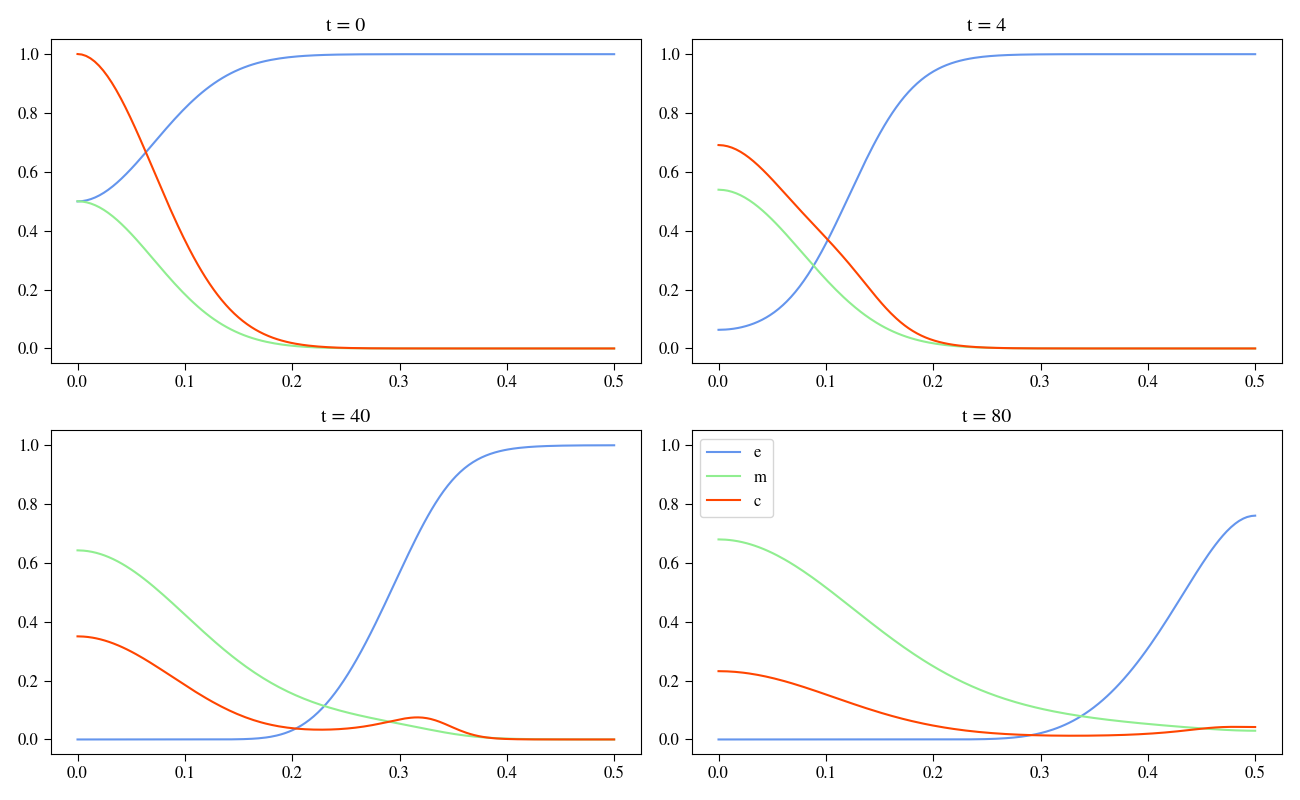
\includegraphics[width=\textwidth]{resources/images/basecase_without_proliferation_.png}
    \caption{Results of using the parameters as described, this experiment will be used as the basecase to compare further experiments to ragarding the model without proliferation and renewal}
    \label{fig:basecase_without_proliferation}
\end{figure}
These adjustments leave us with the final configuration for replicating the system with the curves in figure~\ref{fig:basecase_without_proliferation} and the parameter settings of: $d_c=5\cdot 10^{-4}, \gamma=0.0055, \eta=10, d_m=1\cdot 10^{-3}, \alpha=0.35645, \beta=0$. Comparing our final version with the original experiment we are trying to replicate, figure~\ref{fig:anderson_experiment}, we see the important effects met. We see that the production of the matrix-degrading enzymes fits the original experiment and the motility of the tumor cells also match, with balanced effects of haptotaxis and diffusion.


\subsubsection{Parameter Analysis}
Before we start with the parameter analysis, we will discuss the mathematical intuition concerning the system partial differential equations, equations~\ref{eq:6} to~\ref{eq:10}. \newline The equation governing the tumor cell density incorporates in this version only two coefficients regarding its motility, diffusion and haptotaxis. As mentioned during replicating Anderson et al's experiment, the relation between those two factors determines if a secondary lump of tumor cells seccesses itself from the main lump and invades the tissue at a faster rate than the remaining cells, but also how large this lump will be. We saw this behaviour in figure~\ref{fig:replication_dc_comparison}, varying $d_c$ whilst keeping $\gamma$ constant. Diffusive motility depends on the laplacian of the tumor cells themselves, $\Delta c = \frac{\partial c}{\partial x} + \frac{\partial c}{\partial y} + \frac{\partial c}{\partial z}$, which is a fundamental tool in sciences of all sorts to describe the effects of spacial rate of change of a scalar field quantity, in our case tumor cell density, at a specific point in space. Typically this operator has high values where the respective quantity changes rapidly. For the haptotaxis we have a very similiar term $\nabla \cdot (c\nabla e) = \nabla c \cdot \nabla e + \Delta e$. This means that haptotatic effects are not only strong where the concentration of the extracellular matrix changes rapidly but also where both gradients for tumor cell density and extracellular matrix assimilate in direction, thought these effects can also annihilate each other.\newline 
The equation describing the concentration of the extracellular matrix models exponential decay of it with taking the concentration of the matrix-degrading enzymes into account. In spacial and temporal positions where both ECM and MDE concentrations are high, we can expect a fast degradation of the extracellular matrix.\newline
The equation modelling the matrix-degrading enzymes combines motility with production/decay terms. The motility of the MDEs is modelled by the same diffusion as the tumor cells, mimicking their behaviour in this regard. The tumor cells are responsible for producing the MDEs, the production is modelled by natural decay, both production and decay are modelled using exponential approaches.\newline 
From the replicated results shown in figures~\ref{fig:basecase_without_proliferation}, we saw that if we vary the parameters one at a time the results can vary strongly. We are first going to have a look at how changing one parameter at a time affects the output of the simulation and after this we consider changing multiple parameters simultaneously in the cross variation section. For varying the parameters we assume the other parameters of the system to be constant and use the baseline experiment as their values.

\subsubsection*{$d_c$ Variation}
This parameter describes the diffusive properties of the tumor cells and as Chaplain et al. assumed in~\cite{STEPHANOU200696}, we are also assuming an even distribution of this parameter with $d_c \sim U[1\cdot 10^{-5}, 1\cdot 10^{-3}]$, though in our experiments we encountered numerical instabilities reducing the parameter furhter than $5 \cdot 10^{-5}$. \newline 
As described the intuition is that decreasing $d_c$ will increase the effects haptotaxis and make $\gamma$ more influential. This means the tumor cells will drift faster outward with a bigger secondary lump, forming a pointier leading edge. On the other hand if we increase $d_c$ the effects of haptotaxis will diminish, the tumor cells will be subject to higher diffusion distributing them more evenly in the tissue, additionally there will be less of a secession that is seperated from the main lump of cells. 
\begin{figure}[h!]
    \centering
    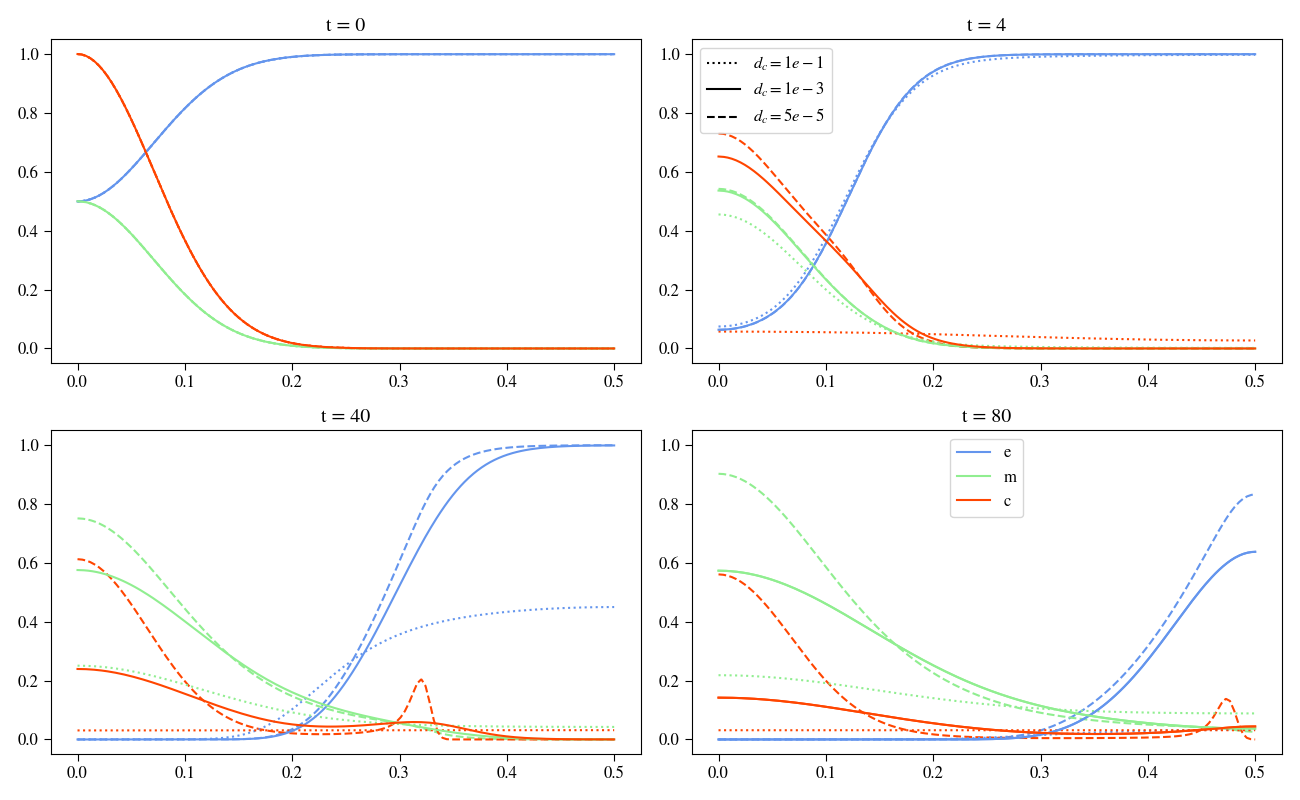
\includegraphics[width=\textwidth]{resources/images/dc_variation.png}
    \caption{Results of varying $d_c$ in the basecase parameter set, keeping the other parameters constant, using the Plot Over Line tool}
    \label{fig:dc_variation}
\end{figure}
Looking at the experiments in figure~\ref{fig:dc_variation}, we can see these assumptions met. The smaller $d_c$ gets the higher the influence of haptotaxis and therefore $\gamma$  will be and vice versa.\newline
Considering the tumor cell denisty curves shown in red, we can after already $t=0.4$ see minor differences. For the two lower values of $d_c$, the solid and dashed curves, we see the tumor cells having a higher concentration at the origin than for the biggest value of $d_c$, dotted curve, nearly overlaying each other. The red dashed curve is considerably lower at the origin though it is stretched  out more than the other two, indicating a faster invasion rate. The other curves describing EDM and MDE concentration don't show any deviations from each other in this point in time.\newline
Looking at the plot results, at time $t=4$, we see the previously observed effects increase. The curves of the tumor cells confirm that with increasing $d_c$ the remaining lump of cells at the origin decreases, distributing the tumor cells more evenly in space and also reducing the effect of haptotaxis, making the secondary lump, that is still visible for the highest diffusion term, less sharp. At this point in time the other two curves also start to show differentiating behaviour. The ECM is degraded faster with increasing $d_c$ and the slope the ECM describes is less steep. Looking at the extracellular matrix we see minor differences in the lower two values for $d_c$. Due to the exponential production of the MDEs by the tumor cells and the more even spread of the tumor cells we see them taking on a lower concentration at the origin, though we can also observe that they have sprach a little bit farther out than the MDE concentrations describing the experiments with lower $d_c$ values.\newline
Studying the last image of $t=8$ we see no new effects, only the already mentioned propagated, with increasing $d_c$ we see a more even spread of the tumor cells and a reduction of the secondary lump leading the invasion of the tissue. For the MDE concentration we observe that there is less concentration in total due to the exponential growth rate, especially at the origin though we also see a more even distribution of them and a slightly faster invasion pace. This causes the extracellular matrix degradation to work faster.\newline 
Regarding the sensitiviy of this parameter, it is to say that the higher the value is, the more sensitive the system reacts. Though the lower two values for $d_c$ are only seperated by $5\cdot 10^{-5}$, and we can unfortunately not experiment with $d_c=1 \cdot 10^{-5}$, due to numerical instabilities, the differences between those two were minimal compared to the difference between the higher two values of $d_c$.\newline 
From a biological point of view this increase of diffusion might be caused by a change of temperature, electric potential or mechanical pressure differences. The higher diffusion results in more even spread of the two actively moving quantities of tumor cells and matrix-degrading enzymes, degrading their surrounding tissue, the ECM, at a faster rate.

\subsubsection*{$\gamma$ Variation}
$\gamma$ describes the effects of haptotaxis, it is assumed that it is evenly distributed in $\gamma \sim U[0.001,0.01]$, like Anderson et al~\cite{anderson_mathematical_2000} assumed. Like Anderson et al. we are also going to look at values exceeding this region though most likely losing their biological meaning. Inspecting the effects of $\gamma$ we can assume the countering effects on the tumor cells as for varying $d_c$; selecting higher values for $\gamma$ will increase the effects of haptotaxis, creating a larger secondary lump of cells that is being pulled faster into the tissue.
\begin{figure}[h!]
    \centering
    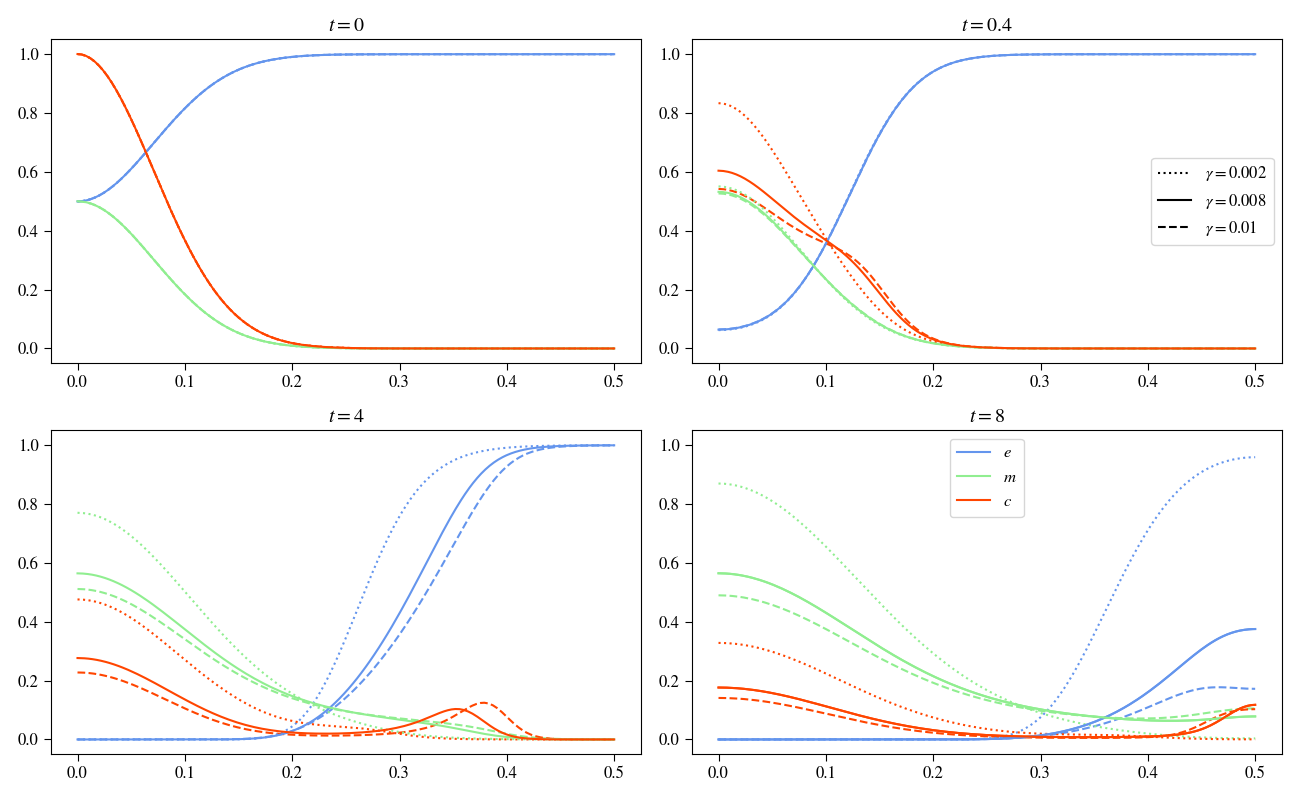
\includegraphics[width=\textwidth]{resources/images/gamma_variation.png}
    \caption{Results of varying $\gamma$ in the basecase parameter set, keeping the other parameters constant, using the Plot Over Line tool}
    \label{fig:gamma_variation}
\end{figure}
The experiments, described in figure~\ref{fig:gamma_variation} verify the expected behaviour.\newline After $t=0.4$ we already see clear changes for varying $\gamma$, the higher $\gamma$ is set, the more of a secession for the tumor cells is observable, that will later from the secondary lump. The lowest value for $\gamma$, undercutting the one for the basecase, shows no signs of a leading edge forming that invades the tissue seperately. The two higher value for $\gamma$ show little deviation at this point in time. Considering the other two variables extracellular matrix concentration and matrix-degrading enzymes concentration, there is no change visible, still overlaying each other at this temporal point.\newline 
The next image shows the simulation after $t=4$ timesteps and here we can clearly see changes in all three variables. 
Whilst the tumor cell density for the values of $0.008$ and $0.01$ differ slightly by the amount of cells that are left at the origin and the distance they have already invaded the surrouding tissue, the curve for the lowest $\gamma$ value, as at $t=0.4$ does not show a secession of the tumor cells that invades the tissue seperately, which causes the tumor cells to stay centered around $x=0$, resulting in a higher denisty of cells there compared to the results of the other experiments. With increasing $\gamma$ the invasion speed also increases, as the dashed line for the tumor cell density shows. For the MDE curve we also observe that the lower $\gamma$ is the more of the concentration is at the origin, which is due to the also higher remaining density of tumor cells at the origin. The ECM concentration shows similiar behaviour as the MDE concentration does, with increasing $\gamma$, the ECM is faster and more evenly degraded, due to the faster invasion of the tissue, the production of matrix-degrading enzymes happens also in regions farther away from the center faster. As we saw varying $d_c$ only little of MDE concentration is needed to efficiently degrade the extracellular matrix, therefore the ECM degradation process happens also faster here.\newline
In the last image at $t=8$ we see the observations from previous points in time confirmed; the higher $\gamma$ the faster the invasion pace of the tumor cells and the more of a secession forms with less tumor cells staying at the origin. The behvviour of the tumor cells causes a higher concentration of MDEs at the origin due to exponential growth and a steeper decline moving outwards. With rising $\gamma$ the ECM is getting degraded faster.\newline 
\begin{figure}[h!]
    \centering
    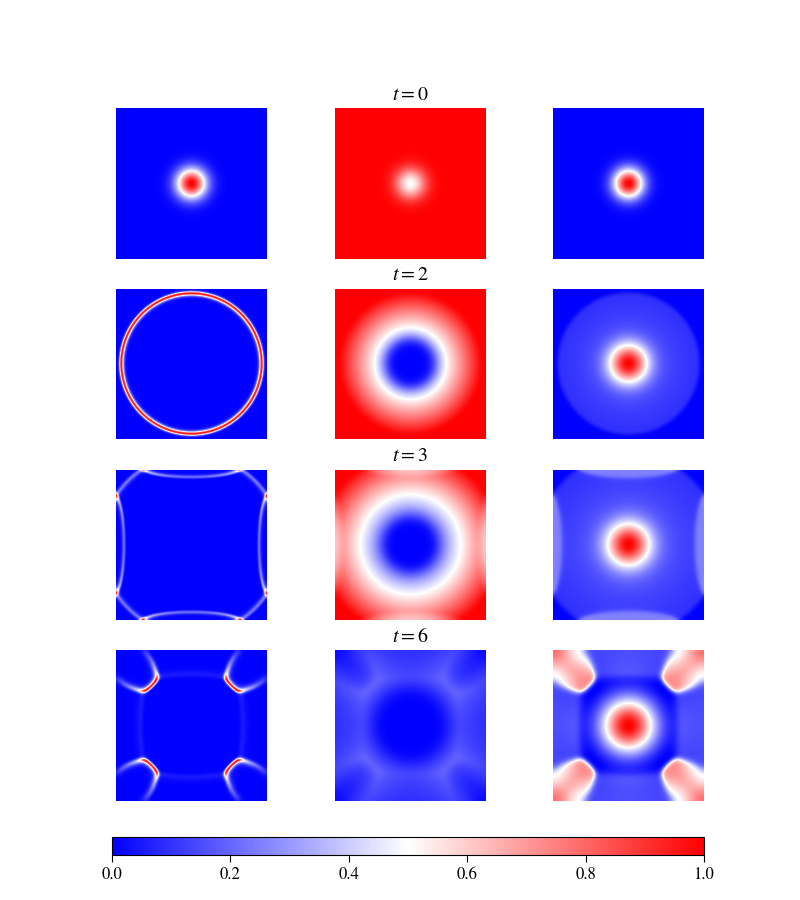
\includegraphics[width=0.85\textwidth]{resources/images/gamma_2D_plot.png}
    \caption{2D plot showing experiment for $\gamma=0.1$, left tumor cell density, right ECM concentration}
    \label{fig:gamma_2D_plot}
\end{figure}
Out of curiousity we are going to take a step further and increase $\gamma$ again by one potence, to $\gamma=0.1$. As previously observed the haptotatic effects pulling the cells into surrounding tissue increase, causing an even faster invasion pace. Yet in this case the invasion pace of the tumor cells is so high there are no cells left at the origin, everything is being pulled into the surrouding tissue. Before finishing the simulation after $t=8$ the tumor cells have reached the border of the doamain $\Omega$. At the border the cells are being reflected, due to the boundry conditions of our model~\ref{eq:9} and~\ref{eq:10}. In figure~\ref{fig:gamma_2D_plot} you can see after $t=2$ the border is reached and at $t=3$ the cells have been reflected to move into the corners, where the ECM concentration is highest. At $t=3$ you can see that the pace of the ECM degradation of the matrix-degrading enzymes has not been able to keep up with the invasion pace of the tumor cells. After being pulled into the corners at $t=3$ and degrading the ECM there, at $t=6$ you see that the tumor cells are being pulled back towards the center of the simulation.\newline
Though this behaviour makes little from a biological perspective, due to the boundry conditions of the system reflecting the movement and the high invasion pace of the tumor cells, it is still interessting to investigate this case, from a numerical perspective.\newline
Though the intuition is met that with increasing $\gamma$ the invasion pace of the tumor cells and matrix-degrading enzymes also rises, we get unexpected behaviour with in the last experiment, there is more of a total ECM concentration left, than in the experiment using $\gamma=0.01$.
Studying those experiments biologically, we know that the term extracellular matrix describes a whole class of different molecules, minearls or proteins, like collagens or enzymes. The different properties of these elements cause varying effects of haptotaxis, for example were the haptotatic effects measured on laminin considerably lower then ones measured on fibronectin, according to Aznavoorian et al.$\textcolor{red}{cite0.1083/jcb.110.4.1427}$. In different sites of the human body there will be different constellations of extracellular matrix composition encountered, which will cause the tumor cells, as seen in the numerical experiments to behave differently.

\subsubsection*{$\eta$ Variation}
The parameter $\eta$ controls the degradation process of the extracellular matrix moluecules. Since Anderson et al~\cite{anderson_mathematical_2000} used a value of $\eta=10$ on all their experiments we assumed an even distributed in $\eta \sim U[0, 20]$. The degradation process of the extracellular matrix is modelled using a exponential decay hypothesis so we can expect that increasing $\eta$ also increases the systems sensitivity with respect to the parameter $\eta$. With its role controlling the degradation it will also heavily influence the motility of the tumor cells and therefore also the motility and production rate of the matrix-degrading enzymes. Slower degradation will results in a higher density of tumor cells at the origin which will exponentially produce matrix-degrading enzymes. Though this in turn will increase the ECM degradation. With increasing $\eta$ the ECM is faster degraded and therefore might provoke a faster invasion rate of the tumor cells of the surrounding tissue. The higher $\eta$ is the less MDEs are needed to efficiently degrade the ECM.\newline
\begin{figure}[h!]
    \centering
    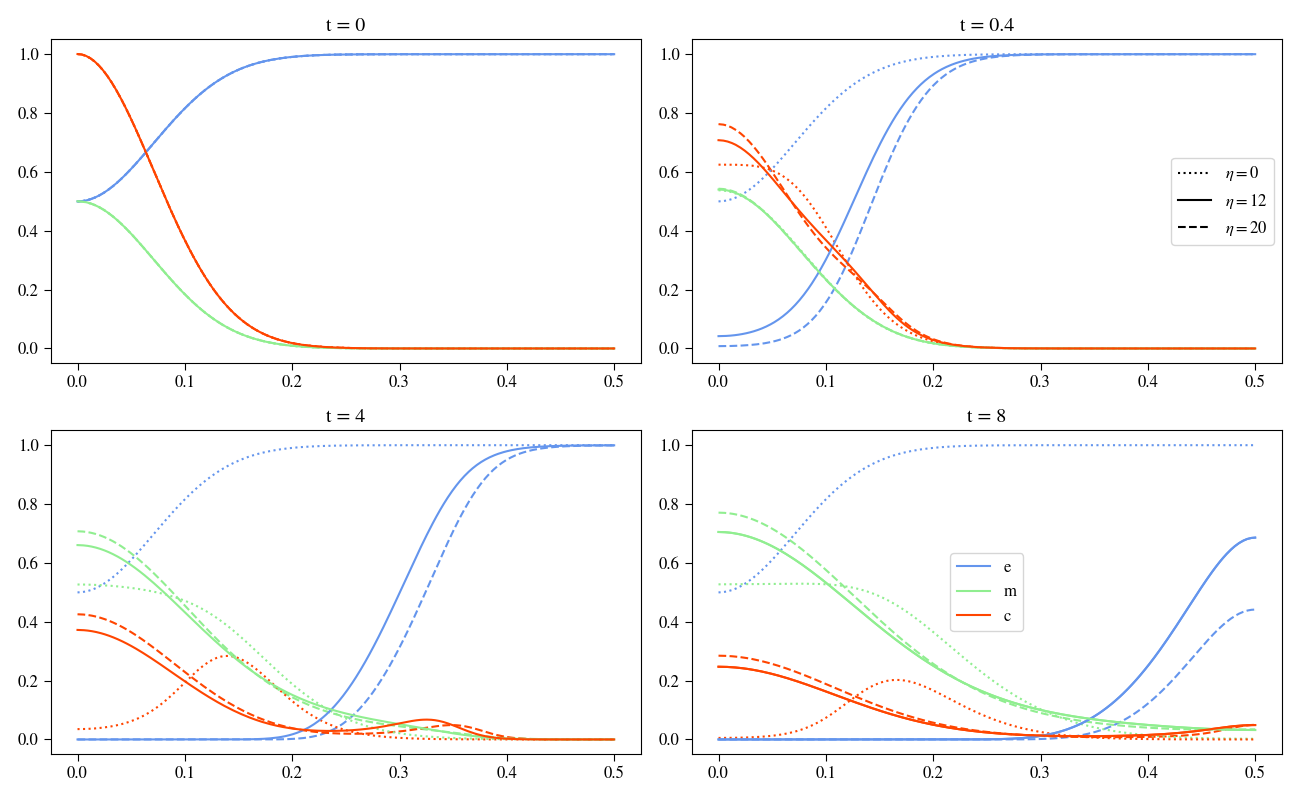
\includegraphics[width=\textwidth]{resources/images/eta_variation.png}
    \caption{Plots show results for varying $\eta$ whilst keeping the other parameters constant, in the images you can see the effects of $\eta=20$ in the dashed curve, $\eta=0$ in the dotted curve and $\eta=12$ in the solid line.}
    \label{fig:eta_variation}
\end{figure}
Inspecting the results in figure~\ref{fig:eta_variation} it is most striking that the slower degradation rate causes a slower tumor invasion. \newline
For both curves tumor cell density and ECM concentration we see after already $t=4$ big differences. Inspecting the experiment with $\eta=2$ we see that the ECM has only degraded a little, which exposed the tumor cells to stronger haptotatic pull by the ECM in regions closer to zero, comparing it to the other experiments. Though it may look like there is no secondary lump of cells being formed, the contrary is the case, even more cells are being pulled into the tissue, with the ECM slower receeding into the tissue. This smoothes out the bump the other two curves for the tumor cell density show. The same effect is observable comparing the tumor cell density curves for the higher $\eta$ values, with less tumor cells being pulled by the ECM the higher $\eta$ gets. Only the curve for the matrix-degrading enzymes has not been affected by the variation of $\eta$ until now.\newline
The next image at $t=4$ propages the effects on the tumor cells and the ECM. The slower the degradation process happens, the more tumor cells invade into the tissue, and the less of a secession is observable. The movement now also affects the concentration of the matrix-degrading enzymes, with the fewer remaining tumor cells at the origin producing less MDEs, yet we see the distribution of the tumor cells for the lowest case of varying $\eta$ with also a more even distribution of MDEs.\newline
The same goes for the last image, showing the experiments at $t=8$. More even tumor cell and matrix-degrading enzymes distribution across space the slower the ECM is degraded.\newline 
As mentioned varying $\gamma$ does the term extracellular matrix include a wide variety of organic or anorganic compounds. The build-up and properties of these compounds therefore vary strongly and motivate this comparison of degradation rate. Some compounds may be degraded faster whilst others are complex needing more time to degrade. 

\subsubsection*{$d_m$ Variation}
\begin{figure}[h]
    \centering
    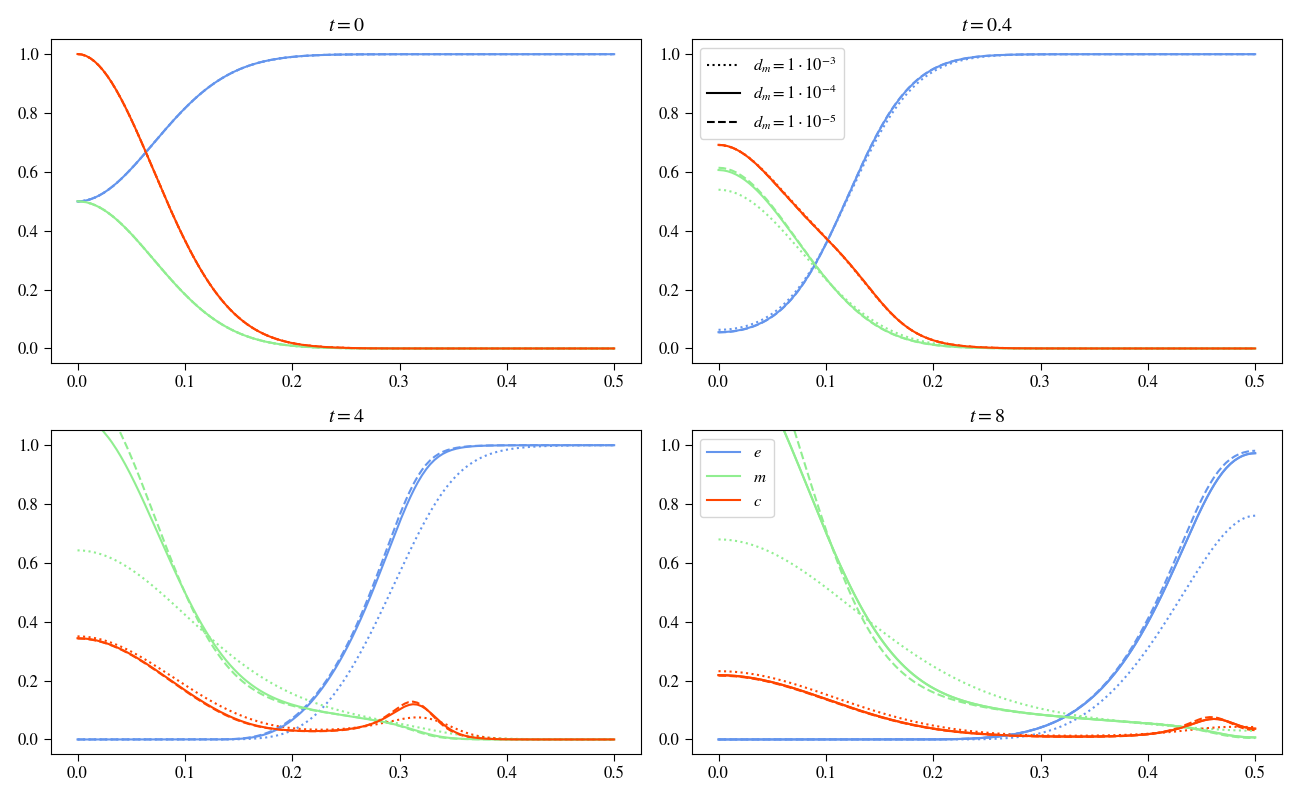
\includegraphics[width=\textwidth]{resources/images/dm_variation.png}
    \caption{Plots show results for varying $d_m$ whilst keeping the other parameters constant, in the images you can see the effects of $d_m=0.1$ in the dashed curve, $d_m=0$ in the dotted curve and $d_m=1\cdot 10^{-3}$ in the solid line.}
    \label{fig:dm_variation}
\end{figure}
$d_m$ is describes the diffusion coefficient of the matrix-degrading enzymes and like for diffusion of the tumor cells we assume it to be evenly distributed with $d_m \sim U[0.00001,0.1]$. Looking at the equations governing the system a faster diffusion of the MDEs into the tissue will cause a faster ECM degradation, since as seen in the experiment varying $d_c$ only little concentration of the matrix-degrading enzymes is needed to efficiently degrade the ECM. Faster ECM degradation will reduce haptotatic effects on the tumor cells, since the pull of it diminishes, causing a slower invasion pace. \newline 
Inspecting the results in figure~\ref{fig:dm_variation} we observe that in the second image after $t=0.4$ for $d_m=0.1$, as for varying the diffusion of the tumor cells, the matrix-degrading enzymes have taken on a constant distribution in space, which as the later point in time show does not change, only the concentration level will increase. This strongly affects the ECM concentration as well, after this short time the ECM has visibly differently than the other for the lower values of $d_m$. Though the overall ECM concentration at this point in time is higher than for the others the degradation happens more evenly moving outward in the unit square. This pregnant change in the ECM concentration shows also in the tumor cell density. The more even degradation of the ECM makes the haptotaxis effects smaller since $\nabla e$ diminishes. As we see the other two curves of the tumor cells developing the secession to form a secondary lump of tumorous cells, we can't see this behaviour here.
For the lower two values we see that as expected higher diffusion causes an more even spread of the matrix-degrading enzymes in space and therefore a lower concentration to stay at the origin. Between those two the effects this has on the ECM degradation and the invasion of the tumor cells are only minor. \newline 
In the next point in time we see that the constant distribution of MDEs in space, causes an a lot faster degradation process of the ECM, in the previous point in time, the total are of the ECM was still larger, here it is visibly lower than for the lower $d_c$ experiments result's. The tumor cells have only slighlty further invaded the tissue though have a more evenly distribution in space. For the MDE concentration we seee that it has visibly rise to a value of approximately $0.1$ everywhere in space. 
Considering the results of the other two experiments at this point in time, we can observe that a very slow diffusion of the matrix-degrading enzymes causes haptotatic effects to increase. This can be explained with the ECM curves, with the one for the lowest $d_m$ experiment is the most steep one, causing high values for $\nabla e$ and therefore a higher haptotaxis value. Interesting to note is that though the ECM degradation happens slowest for the lowest value of $d_m$ the difference between this and the experiment with a value of $d_m=0.00001$ in regard to ECM degradation and tumor cell density vary only slightly, considering a difference of two potentces. Also the difference of the tumor cell density at the origin is for the lower two $d_m$ experiments also only minor, though the MDE concentration here has enormous changes, with the experiment for $d_m$ exceeding one by far, and having a total area that is also far larger. \newline 
The last point in time shows that the high $d_m$ value has caused the ECM to have degraded completly, and has with this eliminated the effects of haptotaxis on the tumor cells, to have them only subject to diffusion. Looking at the other two experiments we observe the same as for the point in time before, lower $d_m$ values result in a less evenly ECM degradation and a considerably higher MDE concentration at the center, which strongly decreases with distance to it. The effects this has on the tumor cells are only minimal, with a higher influence of haptotaxis for lower $d_m$ values. \newline 
Though the differences in the MDE concentration of the lower two $d_m$ experiments are pregnant, the other two curves look roughly the same, while the results with the highest $d_m$ value strongly differ from those. We can conclude that the higher the value of $d_m$ is the more sensitive the system reacts.


\subsubsection*{$\alpha$ Variation}
\begin{figure}[h]
    \centering
    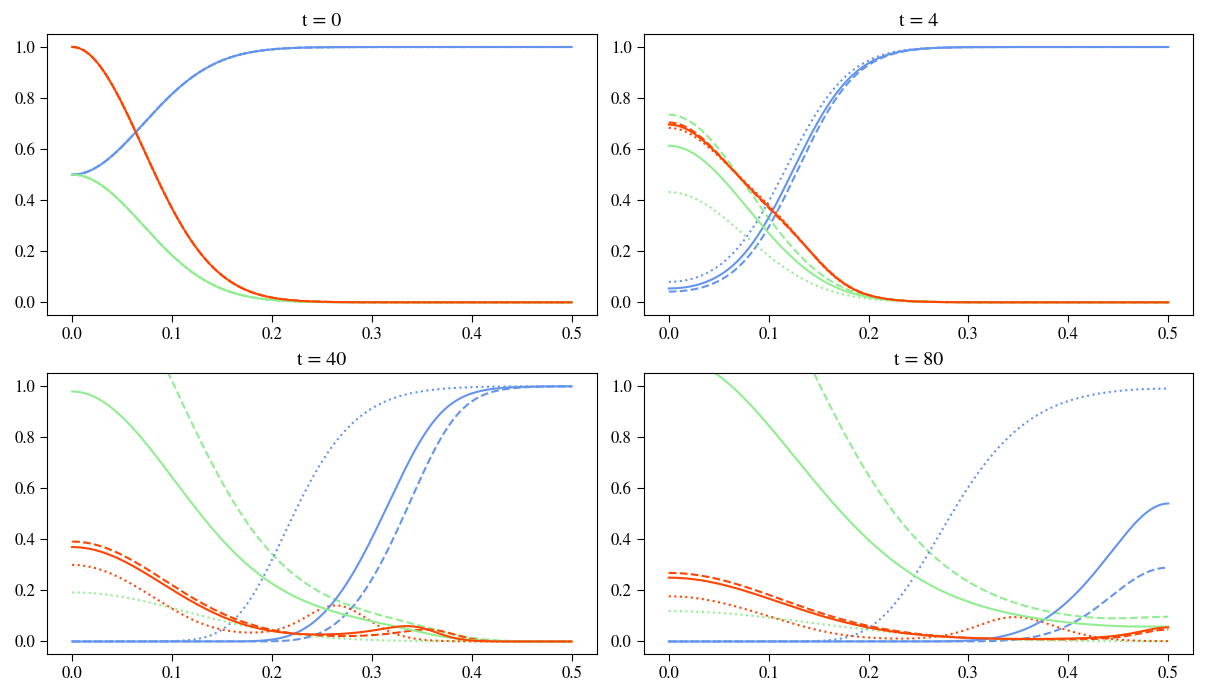
\includegraphics[width=\textwidth]{resources/images/alpha_variation.png}
    \caption{Plots show results for varying $\alpha$ whilst keeping the other parameters constant, in the images you can see the effects of $\alpha=1.0$ in the dashed curve, $\alpha=0$ in the dotted curve and $\alpha=0.6$ in the solid line.}
    \label{fig:alpha_variation}
\end{figure}
The parameter $\alpha$ influences how fast the tumor cells produce matrix decaying enzymes, we assume it to be evenly distributed with $\alpha \sim U[0, 1.0]$. Trying to replicate Anderson et al's experiment we already see how varying $\alpha$ affects the simulation results. With growing $\alpha$ we will see a higher concentration of MDEs especially at the origin. More available MDEs will cause a faster degradation of the ECM first due to having more of them, but also because since more of them are subject to diffusion they will spread faster in the tissue. Faster ECM degrading could mean increased invasion pace of the tumor cells. As we saw in the previous experiments varying $d_c$, the MDE concentration can take on values higher than one, we can also expect this here when $\alpha$ is sufficiently high. \newline 
In the second image of figure~\ref{fig:alpha_variation} describes the experiments after $t=0.4$. We can see that the difference in the MDE curve for the different values of $\alpha$ is already clearly visible, the higher $\alpha$ the higher the concentration of the MDEs. The other curves seem not be affected as strong at this point in time though we can already see differences for th ECM concentration, with a rising degradation pace as $\alpha$ rises. The curve of the tumor cells looks almost identical for all values of $\alpha$, looking very closely we can see small deviations around $x=0$, higher values for $\alpha$ correspond with higher values for the tumor cell density directly at $x=0$, moving further out, as better seen in later points in time, the amount of cells decreases with rising alpha as haptotatic pull is not as strong in this experiment, due to slowed ECM degradation. \newline 
The next point in time at $t=4$, shows the previous mentioned effects in an intensified way. Whilst for $\alpha=0$, the dotted curves, the MDEs have no producing factor and the curve flattens due to diffusion. For the ECM we see that though it has degraded visibly this happened at a slower rate than for the other experiments. The tumor cells have lowest density at the origin of the three experiments, but it's hill at the leading edge has the highest volume, as explained above, due to slowed degradataion the tumor cells at the origin are exposed to higher influences of haptotaxis pulling more of the cells into the surrounding tissue. 
The solid curves describing $\alpha = 0.6$ show that at this point in time they have almost reached a concentration of one at the center, which will be exceeded at the later time steps. With the tumor cells have invaded farther out than in the experiment with the lowest alpha value the ECM degradataion has also been accellerated.
Looking at the dotted lined experiment, $\alpha=1.0$, the value of the MDEs at the origin has already exceeded one by far, with a value of $1,55$ at $x=0$, thus the degradation is happening faster, with a decreased ECM curve and faster invading tumor cells.\newline 
In the last timestep we see that the MDE curve of both $\alpha=0.6$ and $\alpha=1.0$ have exceeded one. The dotted curve of the MDE shows that diffusion has distributed the MDE more evenly throughout space, without changing its overall volume. At the border regions we see that the dotted curve is also the only one that has not yet degraded any ECM in this regions, whilst the dashed curve shows that there is only a little ECM concentration left to degrade for the experiment with the highest $\alpha$ value. This is also shown in the curve of the tumor cells, whilst the dotted curve's peak is still somewhere around $x=0.35$ the other two curves indicate complete invasion of space. \newline
Our initial assumptions are correct with a faster degradation pace due to higher MDE concentration and therefore a faster invasion pace of the tumor cells. Whilst it makes from a numerical perspective sense that the concentration of MDEs can exceed one, it might make sense to introduce a finer grid or adapt the model in other ways, since judging from a continuous perspective it does not really make sense that at a certain point in space there are more than one entities, occupying this space. 

\subsubsection*{$\beta$ Variation}
The variaton of the decay of the matrix-degrading enzymes $\beta$ is shown in figure~\ref{fig:beta_variation}. Using Kolev et al's estimate for $\beta$ in \cite{Kolev2010} we started experimenting with $\beta=0.07$. We therefore settled for an even distribution of $\beta$ in $\beta \sim U[0.005, 0.1]$. Interestingly $\alpha$ and $\beta$ are, as the experiments will confirm, not of the same magnitude, this is caused by the tumor cells having a constant volume in time and the matrix-degrading enzymes to increase over time. We can assume that with varying $\beta$ the MDE curve will be lower, influcencing the ECM degrading process and therefore also the invasion pace. \newline 
\begin{figure}[h]
    \centering
    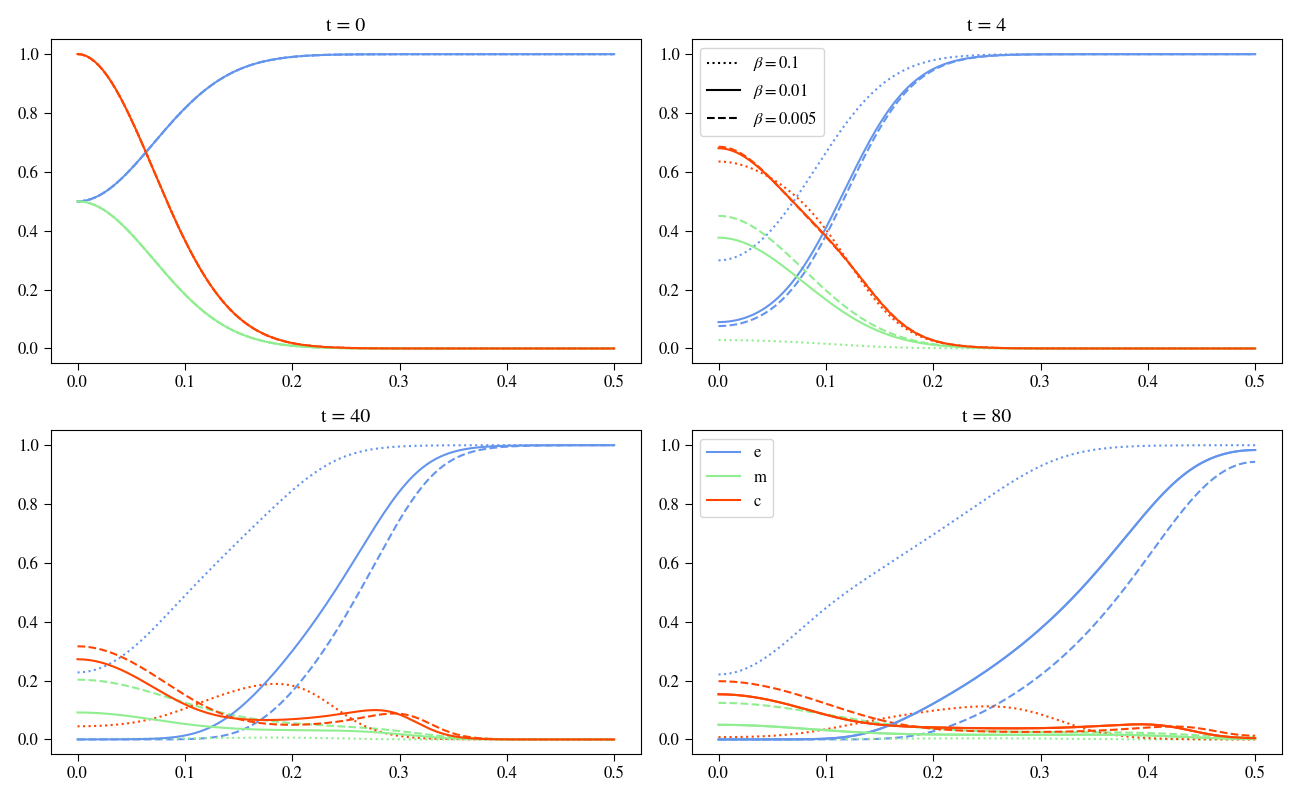
\includegraphics[width=\textwidth]{resources/images/beta_variation.png}
    \caption{Plots show results for varying $\beta$ whilst keeping the other parameters constant, in the images you can see the effects of $\beta=0.005$ in the dashed curve, $\beta=0.1$ in the dotted curve and $\beta=0.01$ in the solid line.}
    \label{fig:beta_variation}
\end{figure}
As we see from the results in figure~\ref{fig:beta_variation} a value of $\beta=0.1$ is sufficient to after already four timesteps reduce the MDE concentration to zero everywhere. In later points in time this decay rate proves to be too high with a curve of MDE concentration everywhere vanishing spacially and temporaly. The immediate decay of the MDEs causes a slower ECM degradation, yet it has no stopped completely since the tumor cells still produce matrix-degrading enzymes. This slow degradation of extracellular matrix causes the tumor cells to remain as one lump of cells, that moves with its maxima in space, below where $\nabla e$ is highest. We saw this effect previously at the variation of $\eta$ where the haptotatic pull of the ECM was kept high at the regions near the center, which also caused to stay as only one lump of cells, with the slow ECM degradation we have the same effect here, though here ECM is still degraded at all.\newline
In the other experiments we can observe that with decreasing $\beta$ and therefore slowing down the decay of the matrix-degrading enzymes, first the ECM degradation accellerates and this causes the effects of haptotaxis and diffusion to develop the two main lumps of tumor cells, one staying at the center the other invading the tissue.
Across all experiments we can say that the ECM degradation happens more evenly with rising $\beta$.
\begin{comment}

We first of all needed to determine a range in which to experiment. Starting with a range of values between $0.1$ and $1.0$, since this is the range $\alpha$ yields reasonable results in and $c$ and $m$ are in the same scale regarding their values, we counter-intuitively saw that those values were much too high. Even for $\beta=0.1$, shown in the dotted curve, the MDEs are almost completely decayed after only $t=4$, leaving only a small portion of MDEs at the origin due to the production from the tumor cells. This makes the ECM degradation process visibly slower and makes the tumor cells a longer time subjected to high effects of haptotaxis, causing to only develop one hill, visible in the red dotted curve.

Looking at the different points in time we can see that though the dotted green MDE curve is nearly everywhere zero we see that degradation still happens visibly and due to the longer exposition on haptotaxis on bigger portions of tumor cells this one lump of cells is being pull through space.
Decreasing to $\beta=0.01$ we see that the for the solid lines in figure~\ref{fig:beta_variation} the MDE concentration takes on higher values througout the points in time. The tumor cells density show again a distinction between the effects of diffusion and haptotaxis, resulting in a two distinctly different lumps with different maxima and ECM degrading resembles most of the previous experiments, though the gradient here is not as steep especilly in the last point in time. 
Further decreasing $\beta$ to $\beta = 0.005$ we see the effects observed in $\beta=0.005$ increase, with a higher concentration of MDEs throughout space and time, and also a faster degradation process. The tumor cells for the dashed curve split into mainly two areas, where the density at the origin is higher than the solid line curve for $\beta=0.01$, and have furhter invaded into the tissue, with a lower density at the leading edge.
Having only one refrence value in Kolev et al's\cite{Kolev2010} paper with $\beta=0.07$ we experimented with this value though saw as we did for $\beta=0.1$ that it was too high distroting the results too strongly, we will further use a range from $0.001$ to $0.01$ to experiment in for $\beta$ as seen in the experiments from figure~\ref{fig:beta_variation}. Here our assumptions were also met, concluding that with rising $\beta$ values the ECM degradation slows down, this also causing the invasion pace of the tumor cells to diminish.
\end{comment}

\subsubsection*{Cross Variation}
Having done all those experiments it will be interesting to see how varying multiple parameters affects the outcome of the simulation. For this we took a look at both supporting and countering effects of variation. 

\subsubsection*{$d_c - \gamma$ Variation}
\begin{figure}[h]
    \centering
    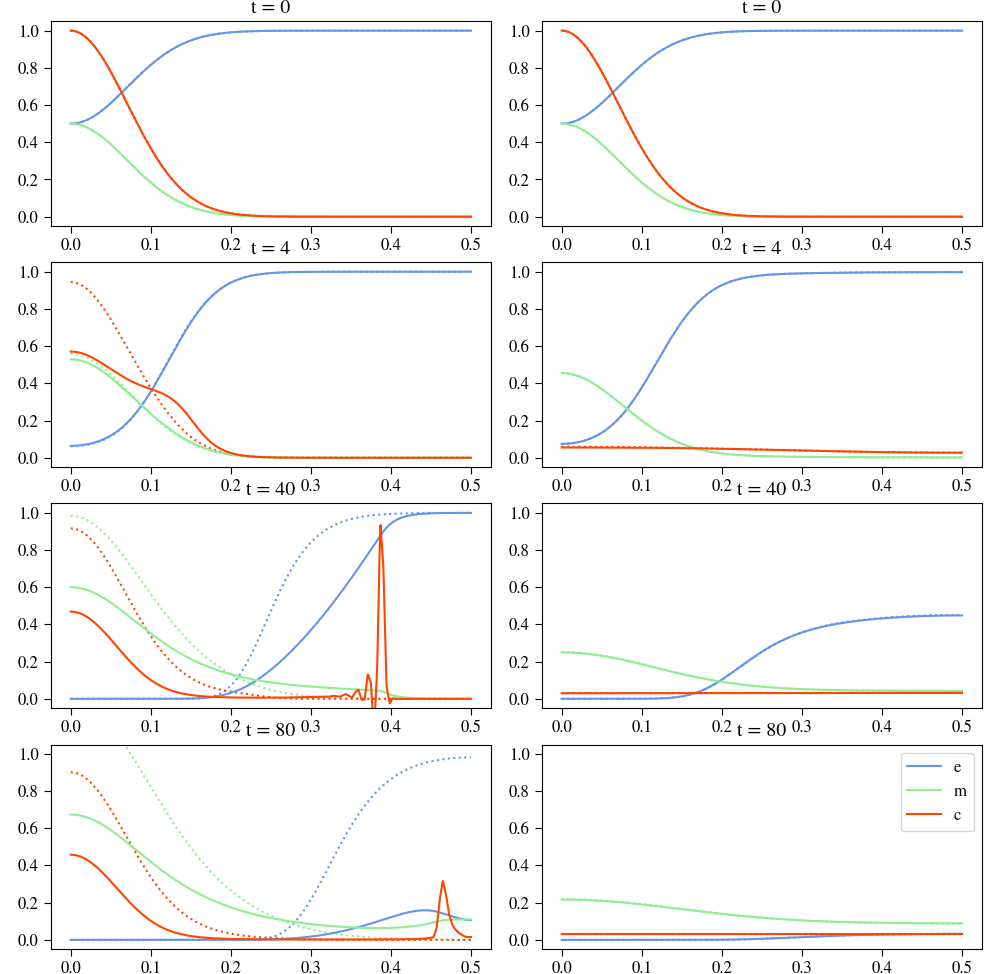
\includegraphics[width=0.85\textwidth]{resources/images/dc_gamma_variation.png}
    \caption{Plots show results for varying both $d_c$ and $\gamma$ whilst keeping the other parameters constant, in the images on the left $d_c$ is set to $d_c=0.00005$ with the solid line showing $\gamma = 0.01$ and the dotted line $\gamma=0.001$ on the right $d_c$ is set to $d_c=0.1$ with the solid line showing $\gamma = 0.01$ and the dotted line $\gamma=0.001$.}
    \label{fig:dc_gamma_variation}
\end{figure}

Having set $d_c=0.00005$ and $\gamma=0.001$ we see no secession of the tumor cells, the effects of haptotaxis are too small leaving the tumor cells only subject to diffusion which results in an even distribution process over time, which also causes a slower invasion pace. Because the tumor cells stay in a lump with its maxima at the origin $x=0$ the MDEs also take on their maximum there, moving farther out they also distribute very evenly. This staying with values around the origin of the MDEs causes a slower ECM degradation. Increasing $\gamma=0.01$ we see that the effects of haptotaxis are now pregnantly visible with a very sharp maxima seen at $t=4$, which equals the maxima of the remaining tumor cell lump at $x=0$. Stronger influence of haptotaxis leads to a faster invasion pace of the tumor cells into the tissue and allowing to create matrix-degrading enzymes in their wake, causing a more even distribution compared to $\gamma=0.001$ and also a faster ECM degrading process. 
Looking at the right side of the plot ~\ref{fig:dc_gamma_variation} we see the results for $d_c=0.1$ here for both $\gamma$ values diffusion overshadows the effects of haptotaxis completely, with after already $t=0.4$ having a constant distribution of tumor cells throughout space. Due to this fast spread of tumor cells, the MDEs are also produced evenly throughout space, and an even faster ECM degradataion. 

\subsubsection*{$d_m - \eta$ Variation}
\begin{figure}[h]
    \centering
    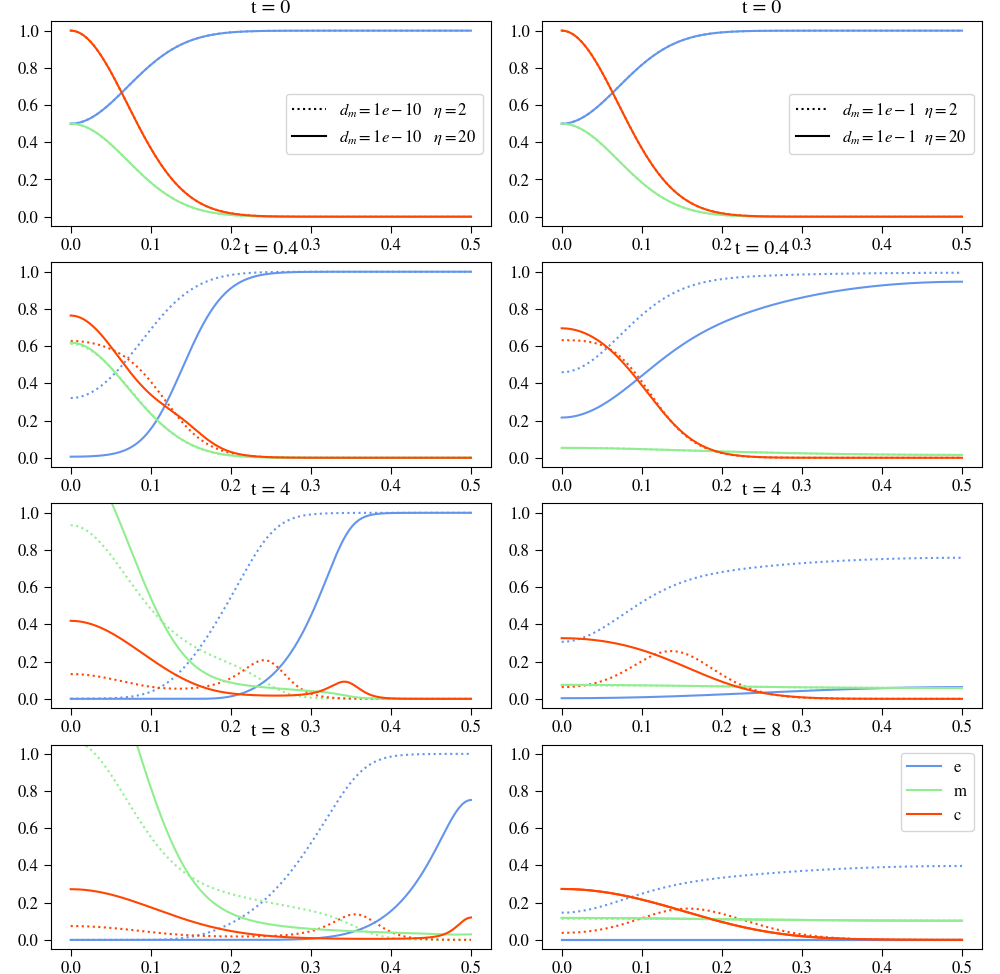
\includegraphics[width=0.85\textwidth]{resources/images/dm_eta_variation.png}
    \caption{Plots show results for varying both $d_m$ and $\eta$ whilst keeping the other parameters constant, in the images on the left $d_m$ is set to $d_m=0.0000000001$ with the solid line showing $\eta = 2$ and the dotted line $\eta=20$ on the right $d_m$ is set to $d_m=0.1$ with the solid line showing $\eta = 2$ and the dotted line $\eta=20$.}
    \label{fig:dm_eta_variation}
\end{figure}

Looking at low values for both $d_m$ and $\eta$ in the figure~\ref{fig:dm_eta_variation}, the dotted curve in the left column, we see that slow diffusion of the matrix-degrading enzymes and slow degradation of the extracellular matrix causes the tumor cells to only develop one lump that invades space, due to stronger haptotatic exposition to a slower degraded ECM, to create larger values for $\nabla (c \nabla e)$, this is also observable for the higher diffusion values and lowwer ECM degrading factors. Having this single lump with a lower maxima and larger length causes the MDEs to produce more evenly farther away from the origin. The low value for the ECM degrading factor results in an overall slower ECM degradation. Looking on the solid line on the left colum we see that increasing $\eta$ enables the tumor cells to develop two hills, one staying at $x=0$ and one invading space by haptotatic pull. Due to a higher density of tumor cells at the origin the MDEs produced there exceed a value of one and ECM degrading happens faster due to first the higher coefficient but also because of a faster invasion pace of matrix-degrading enzymes, due to faster invasion of the tumor cells. Increasing $d_m$ to $d_m=0.1$ causes the MDE concentration to flatten throughout space, taking on a constant distribution in space for one point in time, neglecting the values for $\eta$. Though $\eta$ still has an influence on both tumor cell density and ECM concentration. We see that, as previously mentioned, for $\eta=2$ the degrading happens so slow that the tumor cells form only one lump invading the tissue, with its maxima travelling along the x-axis. In contrast to this for $\eta=20$, we also see only one lump develop though this one stays with it's maxima at the origin. For $\eta=20$ we see that after $t=4$ the ECM has almost completly degraded, making the formation of a secondary lump invading the tissue not possible due to too low haptotatic pull. 

\subsubsection*{$\alpha - \beta$ Variation}
\begin{figure}[h]
    \centering
    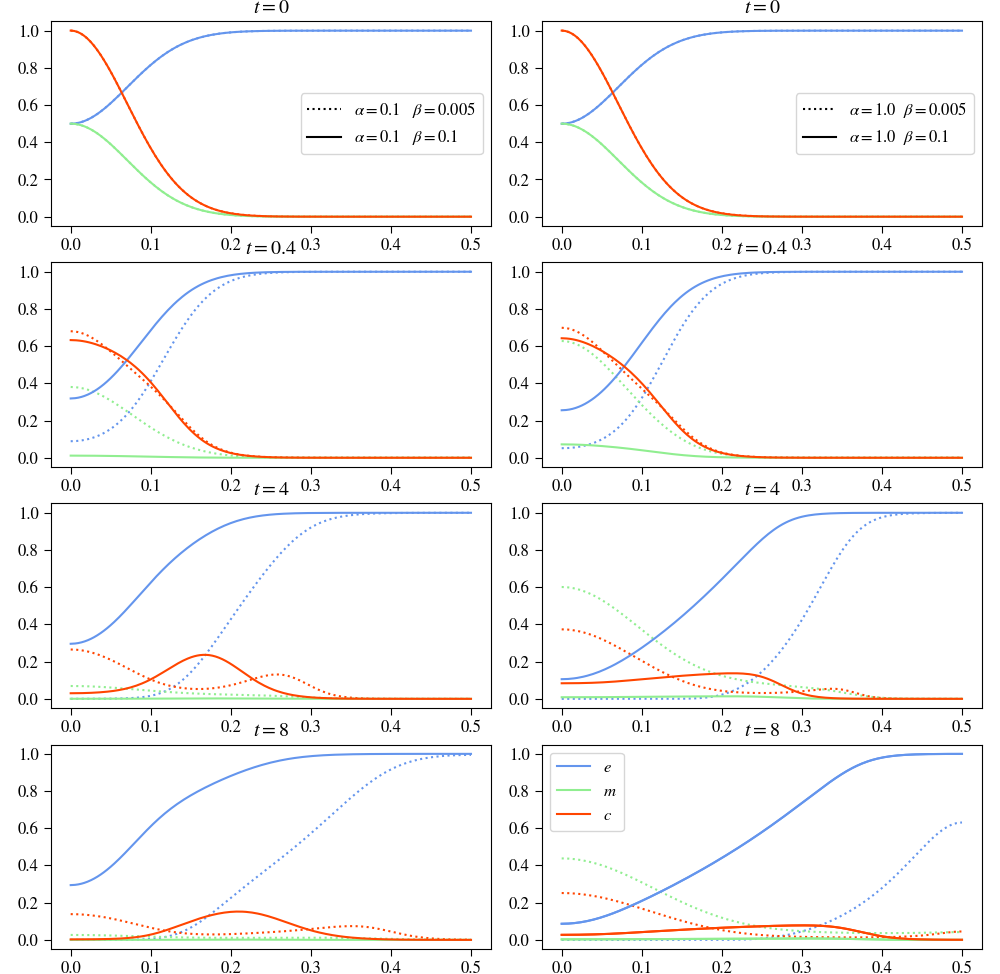
\includegraphics[width=0.85\textwidth]{resources/images/alpha_beta_variation.png}
    \caption{Plots show results for varying both $\alpha$ and $\beta$ whilst keeping the other parameters constant, in the images on the left $\alpha=0.1$ with the solid line showing $\beta = 0.005$ and the dotted line $\beta=0.1$ on the right $\alpha=1.0$ with the solid line showing $\beta = 0.005$ and the dotted line $\beta=0.1$.}
    \label{fig:alpha_beta_variation}
\end{figure}

Looking at figure~\ref{fig:alpha_beta_variation} we see experimental results varying both $\alpha$ and $\beta$. For low MDE production but also low MDE decay we can see that the curve for the MDEs is still visible at up to $t=4$, at $t=8$ it is zero. We see that first the ECM degrading happens faster than for high $\beta$ values and therefore the tumor cells develop two lumps with one invading the tissue the other staying at $x=0$. The maxima for both lumps is lower than in previous experiments, though the cells seem to be more evenly distributed in between the two lumps. Increasing $\beta=0.1$ the MDE curve seems to be zero after already $t=$ and stays there until the end of this experiment. This low concentration of MDEs casuses a slower ECM degrading process and therefore leads the tumor cells to only develop one lump, invading the space, with its maxima moving at the center of this lump. For $\alpha=0.1$ both values for $\beta$ have proven to be to high, decaying the matrix-degrading enzymes too fast to keep up with production.
On the other hand increasing $\alpha$ to $1.0$ and keeping $\beta=0.05$, we see that production outweighs decay, with at the end of the experiment the MDEs still have a concentration of about $0.4$ at $x=0$. For this experiment we seee that the tumor cells develop two lumps indicating that diffusion and haptotaxis effects are also in some balance, and ECM degradation seems to resemble due to similiarities with the basecase for the MDE curve, also the ECM degradation of the basecase experiment.
Increasing both $\alpha$ and $\beta$ we see in the solid line of the right column of figure~\ref{fig:alpha_beta_variation} that decay outweighs production again, after $t=0.4$ we can only see a small remaining portion of matrix-degrading enzymes at the origin. This causes a slower ECM degradataion and therefore to forming only one lump of tumor cells, due to too strong effects of haptotaxis, though this singular lump is streched flat along the x-axis.

\subsubsection*{$d_m - \alpha - \beta$ Variation}
\begin{figure}[h]
    \centering
    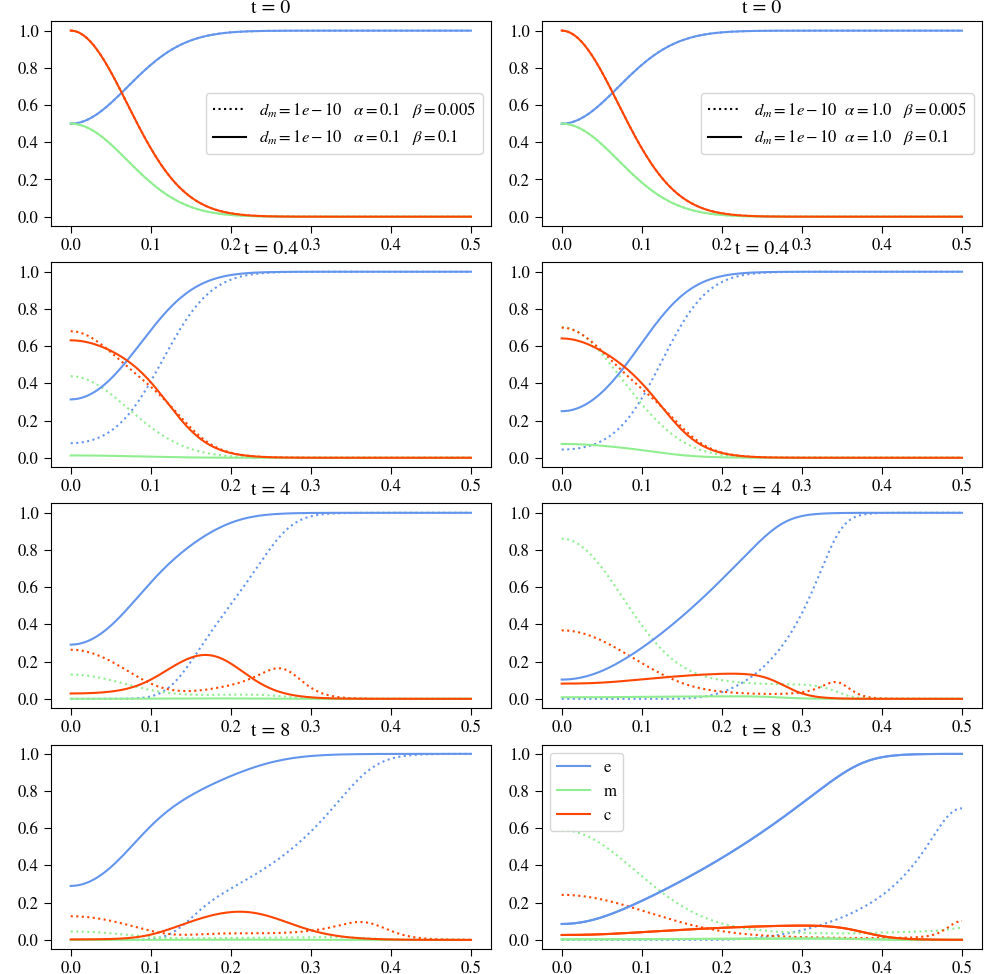
\includegraphics[width=0.85\textwidth]{resources/images/dm_alpha_beta_variation_1.png}
    \caption{Plots show results for varying both $\alpha$ and $\beta$ whilst keeping the other parameters constant, in the images on the left $\alpha=0.1$ with the solid line showing $\beta = 0.005$ and the dotted line $\beta=0.1$ on the right $\alpha=1.0$ with the solid line showing $\beta = 0.005$ and the dotted line $\beta=0.1$.}
    \label{fig:dm_alpha_beta_variation_1}
\end{figure}
\begin{figure}[h]
    \centering
    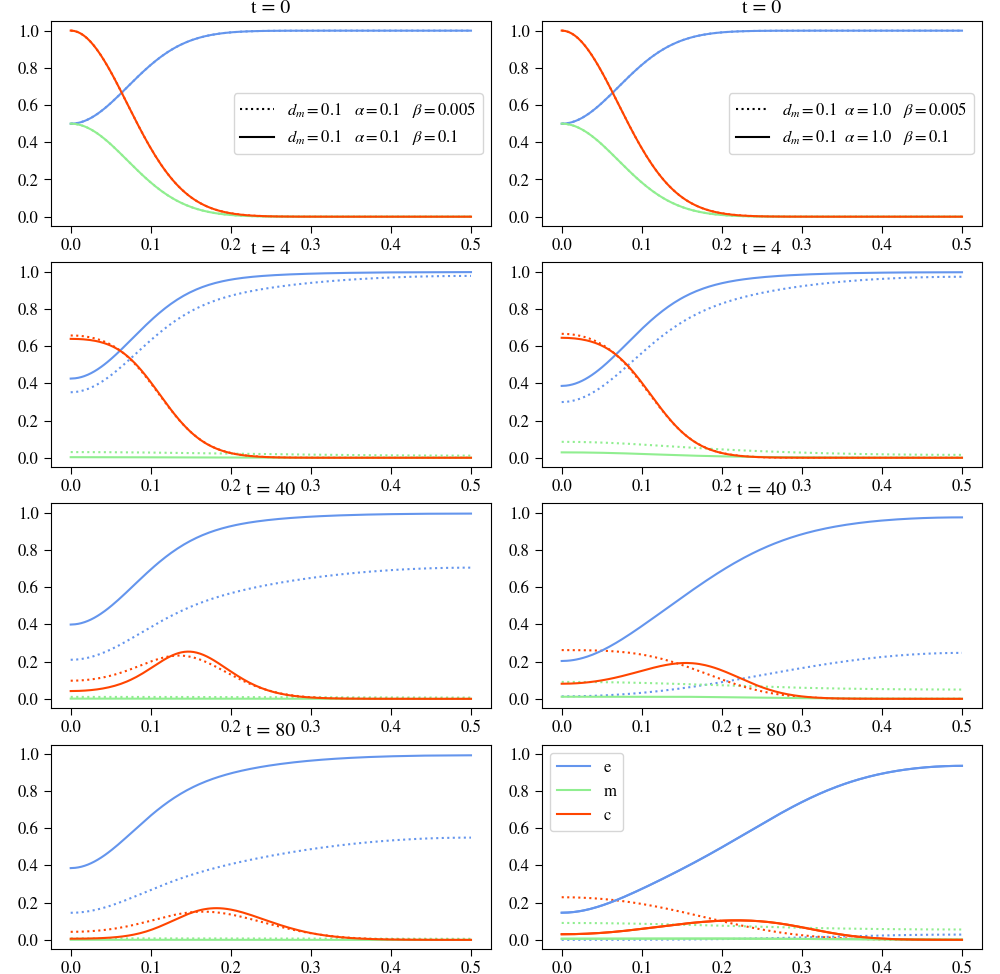
\includegraphics[width=0.85\textwidth]{resources/images/dm_alpha_beta_variation_2.png}
    \caption{Plots show results for varying both $\alpha$ and $\beta$ whilst keeping the other parameters constant, in the images on the left $\alpha=0.1$ with the solid line showing $\beta = 0.005$ and the dotted line $\beta=0.1$ on the right $\alpha=1.0$ with the solid line showing $\beta = 0.005$ and the dotted line $\beta=0.1$.}
    \label{fig:dm_alpha_beta_variation_2}
\end{figure}

Experimenting with all parameters regarding the equation for the matrix-degrading enzymes required to split the results into two figures,~\ref{fig:dm_alpha_beta_variation_1} and ~\ref{fig:dm_alpha_beta_variation_2}, due to clarity reasons. 
We are first going to take a look at the results in figure~\ref{fig:dm_alpha_beta_variation_1}, to see the effect of a decreased diffusion coefficient for the MDEs. We observe that with having $\alpha =0.1$ and $\beta=0.005$ the ECM degradation happens faster due to having a higher MDE concentration, because of lower MDE decay. Which also increases the seperation of the effects of haptotaxis and diffusion on the tumor cells, seperating them into two lumps, one being pulled them along the ECM faster into the tissue the other staying at the origin. Though the MDE concentration diminishes over time we can still see little remaining concentration at the end at $t=8$. Increasing $\beta$ diminishes the MDE concentration sharply, slowing down the ECM degrading process, which increases the effect of haptotaxis over diffusion to pull all of the tumor cells away from the origin to invade the tissue as one lump though at a slower pace. Over time we can see that as expected the tumor cell density's maximum is located approximately right below where $\nabla (c \nabla e)$ is highest. \newline
Looking at the experiments with higher $\alpha$ values we can see that for lower $\beta$ values the MDE concentration oscilates up and down over time, which indicates that with this configuration of $\alpha$ and $\beta$ values we found a balancing point. For higher $\beta$ values we cannot observe this balance, since in this case the MDEs have nearly decayed after $t=4$. Having such differences in the MDE concentration we can also see big differences in the ECM concentration. Here we see that as expected with $\beta=0.005$ the ECM degradation happens a lot faster than having $\beta=0.1$. These changes in the ECM concentration also affect the tumor cell density. Like in the experiments with $\alpha=0.1$ the results for having higher $\beta$ lead to only one lump invading the tissue with a more even distributed density along the x-axis, whereas lower $\beta$ values made the diffusion and haptotaxis differentiable forming two lumps one to stay at the origin, one to invade the tissue outwards.\newline 
Next we are investigating how changing $d_m$ as well will affect the system, looking at figure~\ref{fig:dm_alpha_beta_variation_2}. First of all it is to say that as with varying $d_m$ only the diffusion here is also strong enough to in most cases completely evenly distribute the matrix-degrading enzymes in all of the space after already the fourth step in time. \newline 
On the left side we see the experiments with low $\alpha$ values and see that less decay of the MDEs leads to slower ECM degradataion. Due to the very even distribution of the MDEs we see for both cases a more evenly degradation of the ECM, with overall lower gradients. This results in a longer exposition of haptotatic effects on the tumor cells to form only lump invading the tissue with a moving maximum, though for a lower $\beta$ factor we see that a larger is staying at the origin since the haptotatic pull here is weaker due to having also a more evenly distributed tumor cell density.\newline 
Looking at the right side of figure ~\ref{fig:dm_alpha_beta_variation_2} we see with increased $\alpha$ the results regarding the tumor cell density differ strongly. Whereas on the left side we saw that there was always one lump to invade the cells with its maximum moving below where $\nabla(c\nabla e)$ is strongest, we see that for low $\beta$ the lump of tumor cell stays with its core at the origin at $x=0$, where also its maximum is, and invades the tissue with no leading edge. This shows the effect of a both sufficiently fast and efficient degradation of extracellular matrix. Here we see diffusion as the main factor for the movement of the tumor cells since the haptotatic pull is very low, due to small gradients of $e$ only. For the other curves we can observe that as before with rising $\beta$ the ECM degradation pace slows down, in the last point in time the difference $\beta$ causes is pregnantly visible with for low $\beta$ the ECM has been degraded completely but for high $\beta$ there is still a considerable concentration. Looking at the MDE concentration we can also see clear differences regarding the influence of the diffusion on the MDE decay. Though the MDE concentration with high diffusion is more evenly distributed, its overall volume in space is clearly lower than for low diffusion terms, with same $\alpha$ and $\beta$ configuarations.



\subsection{Two dimensional Results with Proliferation and Renewal}
In this section we are going to inspect the updated system, consisting of equation ~\ref{eq:6} to ~\ref{eq:10}. They describe the effects of tumor cell proliferation and extracellular matrix renewal processes. Like for the model neglecting proliferation and renewal we can see in table~\ref{table:2D_experiments_with_proliferation} all the experiments done in two space dimensions using the updated model. We are going perform a parameter analysis with the same values as done above to make the observed effects pregnant.\newline
As in section~\ref{sec:2D_without_proliferation}, we are using the same inital conditions for all three variables under the assumption we have a homogenous ECM structure. Figure~\ref{fig:2D_homogenous_ECM_initial} depicts these initial conditions on the three variables $c,e,m$ at dimensionless time $t=0$.
\begin{longtable}{|c c c c c c c c c c|}
    \hline
    Figure & Linestyle & $d_c$ & $\gamma$ & $\mu_1$ & $\eta$ & $\mu_2$ & $d_m$ & $\alpha$ & $\beta$ \\ [0.5ex] 
    \hline\hline
    \endfirsthead
    \hline
    Figure & Linestyle & $d_c$ & $\gamma$ & $\mu_1$ & $\eta$ & $\mu_2$ & $d_m$ & $\alpha$ & $\beta$ \\ [0.5ex] 
    \hline\hline
    \endhead
    \hline \multicolumn{10}{|r|}{{continued on next page}} \\ \hline
    \endfoot
    \endlastfoot
    \ref{fig:2D_basecase_comparison} & \sampleline{dotted} & $5\cdot 10^{-4}$ & 0.0055 & 0 & 10 & 0 & $1\cdot 10^{-3}$ & 0.3564 & 0\\ \hline
    \ref{fig:2D_basecase_comparison} & \sampleline{} & $5\cdot 10^{-4}$ & 0.0055 & 0.1 & 10 & 0.5 & $1\cdot 10^{-3}$ & 0.3564 & 0\\ \hline
    \ref{fig:prolif_dc_comparison} & \sampleline{dotted} & $1\cdot 10^{-3}$ & 0.0055 & 0.1 & 10 & 0.5 & $1\cdot 10^{-3}$ & 0.3564 & 0 \\ \hline
    \ref{fig:prolif_dc_comparison} & \sampleline{} & $1\cdot 10^{-4}$ & 0.0055 & 0.1 & 10 & 0.5 & $1\cdot 10^{-3}$ & 0.3564 & 0 \\ \hline 
    \ref{fig:prolif_dc_comparison} & \sampleline{dashed} & $5\cdot 10^{-5}$ & 0.0055 & 0.1 & 10 & 0.5 & $1\cdot 10^{-3}$ & 0.3564 & 0 \\ \hline
    \ref{fig:prolif_gamma_variation} & \sampleline{dotted} & $5\cdot 10^{-4}$ & 0.002 & 0.1 & 10 & 0.5 & $1\cdot 10^{-3}$ & 0.3564 & 0\\  \hline
    \ref{fig:prolif_gamma_variation} & \sampleline{} & $5\cdot 10^{-4}$ & 0.008 & 0.1 & 10 & 0.5 & $1\cdot 10^{-3}$ & 0.3564 & 0\\  \hline
    \ref{fig:prolif_gamma_variation} & \sampleline{dashed} & $5\cdot 10^{-4}$ & 0.01 & 0.1 & 10 & 0.5 & $1\cdot 10^{-3}$ & 0.3564 & 0\\  \hline
    \ref{fig:prolif_mu_1_variation} & \sampleline{dotted} & $5\cdot 10^{-4}$ & 0.0055 & 0 & 10 & 0.5 & $1\cdot 10^{-3}$ & 0.3564 & 0\\  \hline
    \ref{fig:prolif_mu_1_variation} & \sampleline{} & $5\cdot 10^{-4}$ & 0.0055 & 0.5 & 10 & 0.5 & $1\cdot 10^{-3}$ & 0.3564 & 0\\  \hline
    \ref{fig:prolif_mu_1_variation} & \sampleline{dashed} & $5\cdot 10^{-4}$ & 0.0055 & 1.0 & 10 & 0.5 & $1\cdot 10^{-3}$ & 0.3564 & 0\\ \hline
    \ref{fig:prolif_eta_variation} & \sampleline{dotted} & $5\cdot 10^{-4}$ & 0.0055 & 0.1 & 2 & 0.5 & $1\cdot 10^{-3}$ & 0.3564 & 0\\  \hline
    \ref{fig:prolif_eta_variation} & \sampleline{} & $5\cdot 10^{-4}$ & 0.0055 & 0.1 & 12 & 0.5 & $1\cdot 10^{-3}$ & 0.3564 & 0\\  \hline
    \ref{fig:prolif_eta_variation} & \sampleline{dashed} & $5\cdot 10^{-4}$ & 0.0055 & 0.1 & 20 & 0.5 & $1\cdot 10^{-3}$ & 0.3564 & 0\\ \hline
    \ref{fig:prolif_mu_2_variation} & \sampleline{dotted} & $5\cdot 10^{-4}$ & 0.0055 & 0.1 & 10 & 0.1 & $1\cdot 10^{-3}$ & 0.3564 & 0\\ \hline
    \ref{fig:prolif_mu_2_variation} & \sampleline{} & $5\cdot 10^{-4}$ & 0.0055 & 0.1 & 10 & 0.6 & $1\cdot 10^{-3}$ & 0.3564 & 0\\  \hline
    \ref{fig:prolif_mu_2_variation} & \sampleline{dashed} & $5\cdot 10^{-4}$ & 0.0055 & 0.1 & 10 & 1.0 & $1\cdot 10^{-3}$ & 0.3564 & 0\\ \hline
    \ref{fig:prolif_dm_variation} & \sampleline{dotted} & $5\cdot 10^{-4}$ & 0.0055 & 0.1 & 10 & 0.5 & $1\cdot 10^{-3}$ & 0.3564 & 0\\ \hline
    \ref{fig:prolif_dm_variation} & \sampleline{} & $5\cdot 10^{-4}$ & 0.0055 & 0.1 & 10 & 0.5 & $1\cdot 10^{-4}$ & 0.3564 & 0\\  \hline
    \ref{fig:prolif_dm_variation} & \sampleline{dashed} & $5\cdot 10^{-4}$ & 0.0055 & 0.1 & 10 & 0.5 & $1\cdot 10^{-5}$ & 0.3564 & 0\\  \hline
    \ref{fig:prolif_alpha_variation} & \sampleline{dotted} & $5\cdot 10^{-4}$ & 0.0055 & 0.1 & 10 & 0.5 & $1\cdot 10^{-3}$ & 0 & 0 \\ \hline
    \ref{fig:prolif_alpha_variation} & \sampleline{} & $5\cdot 10^{-4}$ & 0.0055 & 0.1 & 10 & 0.5 & $1\cdot 10^{-3}$ & 0.6 & 0 \\ \hline
    \ref{fig:prolif_alpha_variation} & \sampleline{dashed} & $5\cdot 10^{-4}$ & 0.0055 & 0.1 & 10 & 0.5 & $1\cdot 10^{-3}$ & 1.0 & 0 \\ \hline
    \ref{fig:prolif_beta_variation} & \sampleline{dotted} & $5\cdot 10^{-4}$ & 0.0055 & 0.1 & 10 & 0.5 & $1\cdot 10^{-3}$ & 0.3564 & 0.1 \\ \hline
    \ref{fig:prolif_beta_variation} & \sampleline{} & $5\cdot 10^{-4}$ & 0.0055 & 0.1 & 10 & 0.5 & $1\cdot 10^{-3}$ & 0.3564 & 0.01 \\ \hline
    \ref{fig:prolif_beta_variation} & \sampleline{dashed} & $5\cdot 10^{-4}$ & 0.0055 & 0.1 & 10 & 0.5 & $1\cdot 10^{-3}$ & 0.3564 & 0.005 \\ \hline
    \ref{fig:prolif_mu_1_mu_2_variation} - left & \sampleline{dotted} & $5\cdot 10^{-4}$ & 0.0055 & 0.1 & 10 & 0.1 & $1\cdot 10^{-3}$ & 0.3564 & 0 \\ \hline
    \ref{fig:prolif_mu_1_mu_2_variation} - left & \sampleline{} & $5\cdot 10^{-4}$ & 0.0055 & 0.1 & 10 & 1.0 & $1\cdot 10^{-3}$ & 0.3564 & 0 \\ \hline
    \ref{fig:prolif_mu_1_mu_2_variation} - right & \sampleline{dotted} & $5\cdot 10^{-4}$ & 0.0055 & 1.0 & 10 & 0.1 & $1\cdot 10^{-3}$ & 0.3564 & 0 \\ \hline
    \ref{fig:prolif_mu_1_mu_2_variation} - right & \sampleline{} & $5\cdot 10^{-4}$ & 0.0055 & 1.0 & 10 & 1.0 & $1\cdot 10^{-3}$ & 0.3564 & 0 \\ \hline
    \ref{fig:prolif_dc_gamma_mu_1_variation_1} - left & \sampleline{dotted} & $1\cdot 10^{-5}$ & 0.001 & 0.1 & 10 & 0.5 & $1\cdot 10^{-3}$ & 0.3564 & 0 \\ \hline
    \ref{fig:prolif_dc_gamma_mu_1_variation_1} - left & \sampleline{} & $1\cdot 10^{-5}$ & 0.001 & 1.0 & 10 & 0.5 & $1\cdot 10^{-3}$ & 0.3564 & 0 \\ \hline
    \ref{fig:prolif_dc_gamma_mu_1_variation_1} - right & \sampleline{dotted} & $1\cdot 10^{-5}$ & 0.01 & 0.1 & 10 & 0.5 & $1\cdot 10^{-3}$ & 0.3564 & 0 \\ \hline
    \ref{fig:prolif_dc_gamma_mu_1_variation_1} - right & \sampleline{} & $1\cdot 10^{-5}$ & 0.01 & 1.0 & 10 & 0.5 & $1\cdot 10^{-3}$ & 0.3564 & 0 \\ \hline
    \ref{fig:prolif_dc_gamma_mu_1_variation_2} - left & \sampleline{dotted} & $1\cdot 10^{-3}$ & 0.001 & 0.1 & 10 & 0.5 & $1\cdot 10^{-3}$ & 0.3564 & 0 \\ \hline
    \ref{fig:prolif_dc_gamma_mu_1_variation_2} - left & \sampleline{} & $1\cdot 10^{-3}$ & 0.001 & 1.0 & 10 & 0.5 & $1\cdot 10^{-3}$ & 0.3564 & 0 \\ \hline
    \ref{fig:prolif_dc_gamma_mu_1_variation_2} - right & \sampleline{dotted} & $1\cdot 10^{-3}$ & 0.01 & 0.1 & 10 & 0.5 & $1\cdot 10^{-3}$ & 0.3564 & 0 \\ \hline
    \ref{fig:prolif_dc_gamma_mu_1_variation_2} - right & \sampleline{} & $1\cdot 10^{-3}$ & 0.01 & 1.0 & 10 & 0.5 & $1\cdot 10^{-3}$ & 0.3564 & 0 \\ \hline
    \ref{fig:prolif_eta_mu_2_variation} - left & \sampleline{dotted} & $5\cdot 10^{-4}$ & 0.0055 & 0.1 & 2 & 0.1 & $1\cdot 10^{-3}$ & 0.3564 & 0 \\ \hline
    \ref{fig:prolif_eta_mu_2_variation} - left & \sampleline{} & $5\cdot 10^{-4}$ & 0.0055 & 0.1 & 2 & 1.0 & $1\cdot 10^{-3}$ & 0.3564 & 0 \\ \hline
    \ref{fig:prolif_eta_mu_2_variation} - right & \sampleline{dotted} & $5\cdot 10^{-4}$ & 0.0055 & 0.1 & 20 & 0.1 & $1\cdot 10^{-3}$ & 0.3564 & 0 \\ \hline
    \ref{fig:prolif_eta_mu_2_variation} - right & \sampleline{} & $5\cdot 10^{-4}$ & 0.0055 & 0.1 & 20 & 1.0 & $1\cdot 10^{-3}$ & 0.3564 & 0 \\ \hline
    \caption{Overview of all experiments conducted for the model with proliferation and renewal producing 2D output}
    \label{table:2D_experiments_with_proliferation}
\end{longtable}


\subsubsection*{Basecase Analysis}

\begin{figure}[h]
    \centering
    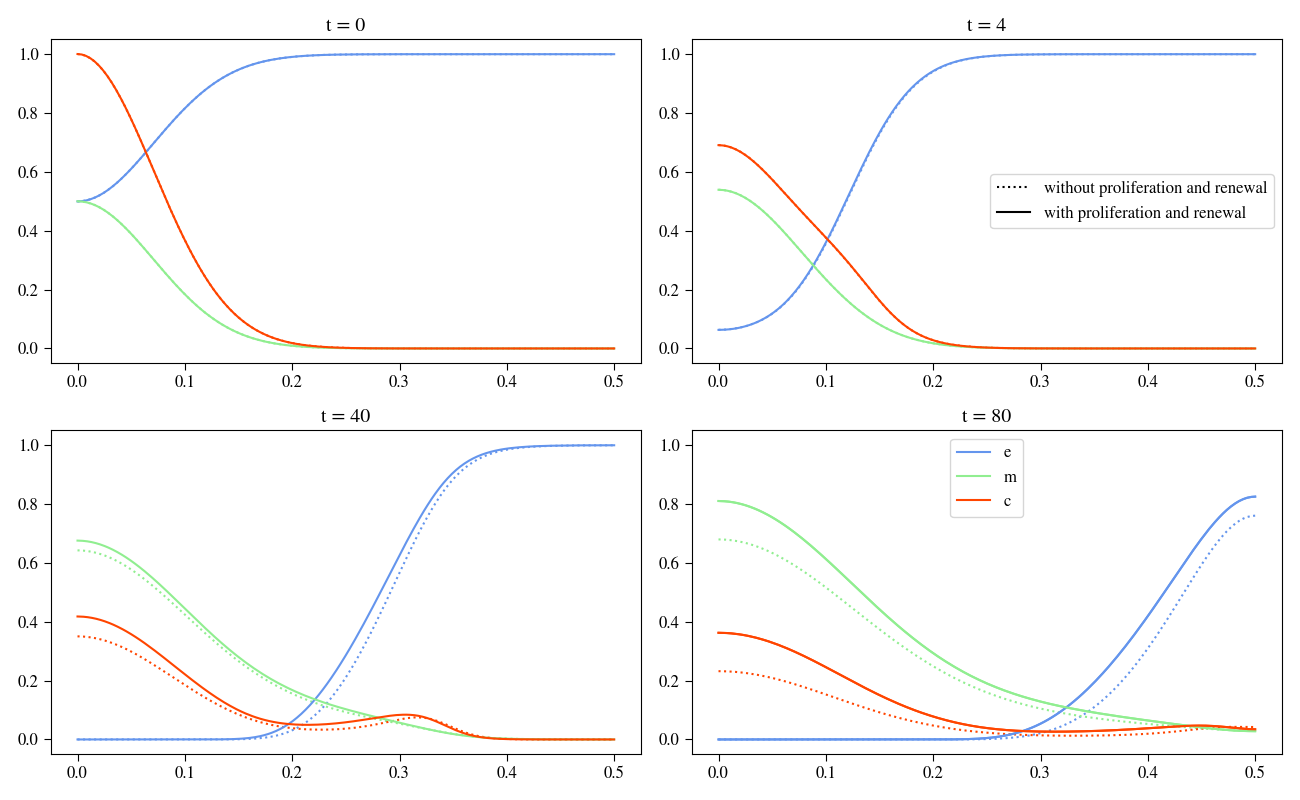
\includegraphics[width=\textwidth]{resources/images/basecase_comparison.png}
    \caption{Describing the updated basecase, in the image above only the updated basecase is plotted, below it is compared to the initial basecase.}
    \label{fig:2D_basecase_comparison}
\end{figure}

It makes sense to establish a basecase to compare the following parameter analysis resulst against it. In figure~\ref{fig:2D_basecase_comparison} you can see how intoducting tumor cell proliferation and extracellular matrix renewal changes the outcome of the simulation. For this we used the values $\mu_1= 0.1$ and $\mu_2=0.5$ according to the only experiment found for this system of equations in the paper of Kolev et al. \cite{Kolev2010}.\newline
Comparing this new basecase to our initial model's basecase we can see the influences of both $\mu_1$ and $\mu_2$, as for the tumor cell density curve is visibly higher than without proliferation, causing a higher production of matrix-degrading enzymes, which would lead to faster ECM degradation, though this is countered by the renewal factor $\mu_2$ causing the ECM concentration to be higher at the end, at $t=8$, than in the initial basecase experiment.




\subsubsection{Parameter Analysis}

For the Parameter Analysis of the model with proliferation and renewal we are focusing on comparing the results of the updated model with the results produced by the model without renewal and proliferation, this will point out again the influence of $\mu_1$ and $\mu_2$ on the system. 

\subsubsection*{$d_c$ Variation}
\begin{figure}[h]
    \centering
    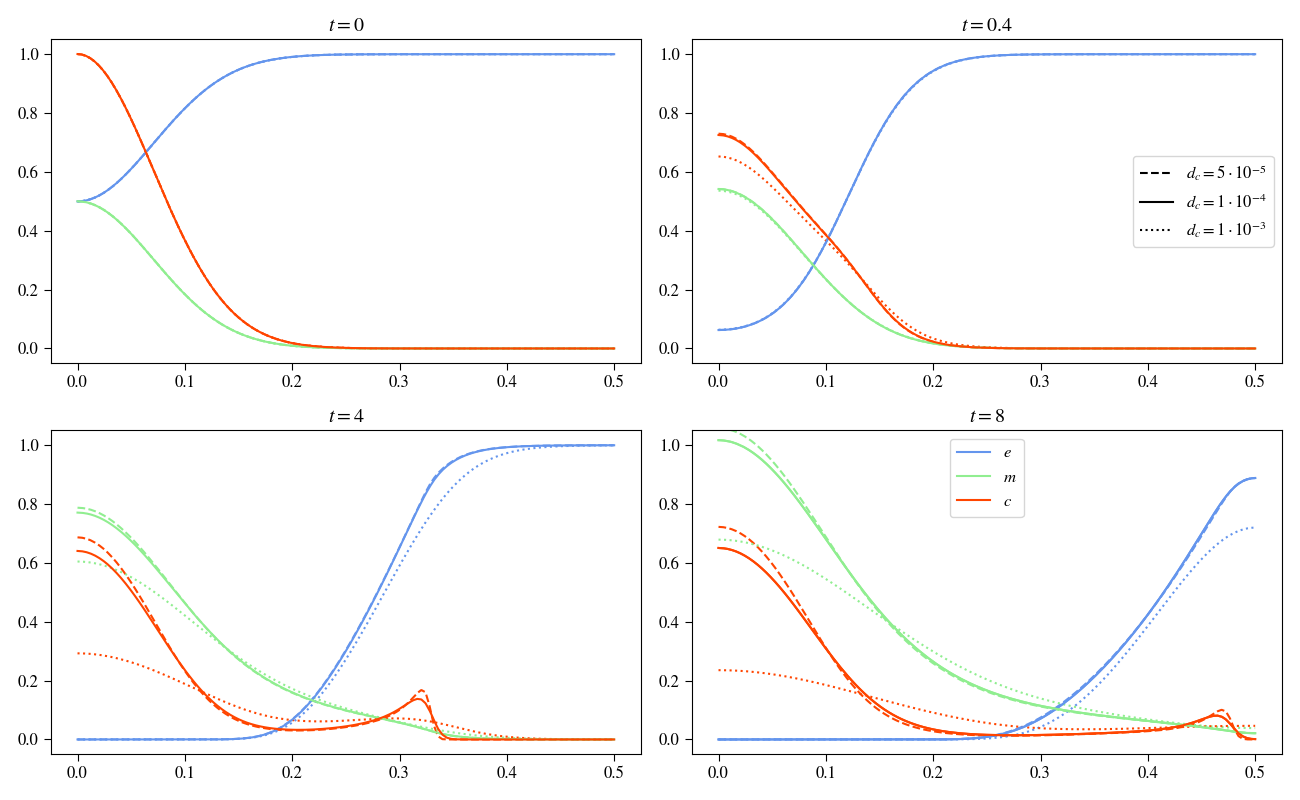
\includegraphics[width=\textwidth]{resources/images/prolif_dc_variation.png}
    \caption{Plots show results for varying $d_c$ whilst keeping the other parameters constant}
    \label{fig:prolif_dc_comparison}
\end{figure}

Varying $d_c$ with proliferation terms, we see the same effects as without proliferation. Higher values for $d_c$ cause a stronger influence of diffusion and a weaker for the haptotaxis, which leads to a curve with less or none of a leading edge invading the space, but to a faster rather constant distribution throughout space. The MDE concentration follows this behaviour, depending on its production on the tumor cell density distribution in space and the ECM is decayed faster, the faster the tissue is invaded, thus the higher the diffusion factor is. Comparing them we see little differences, only tumor cell density and ECM are raised a little in each plot due to the renewal and proliferation factors, which in turn also causes a higher MDE concentration, due to higher tumor cell densities. 


\subsubsection*{$\gamma$ Variation}

\begin{figure}[h]
    \centering
    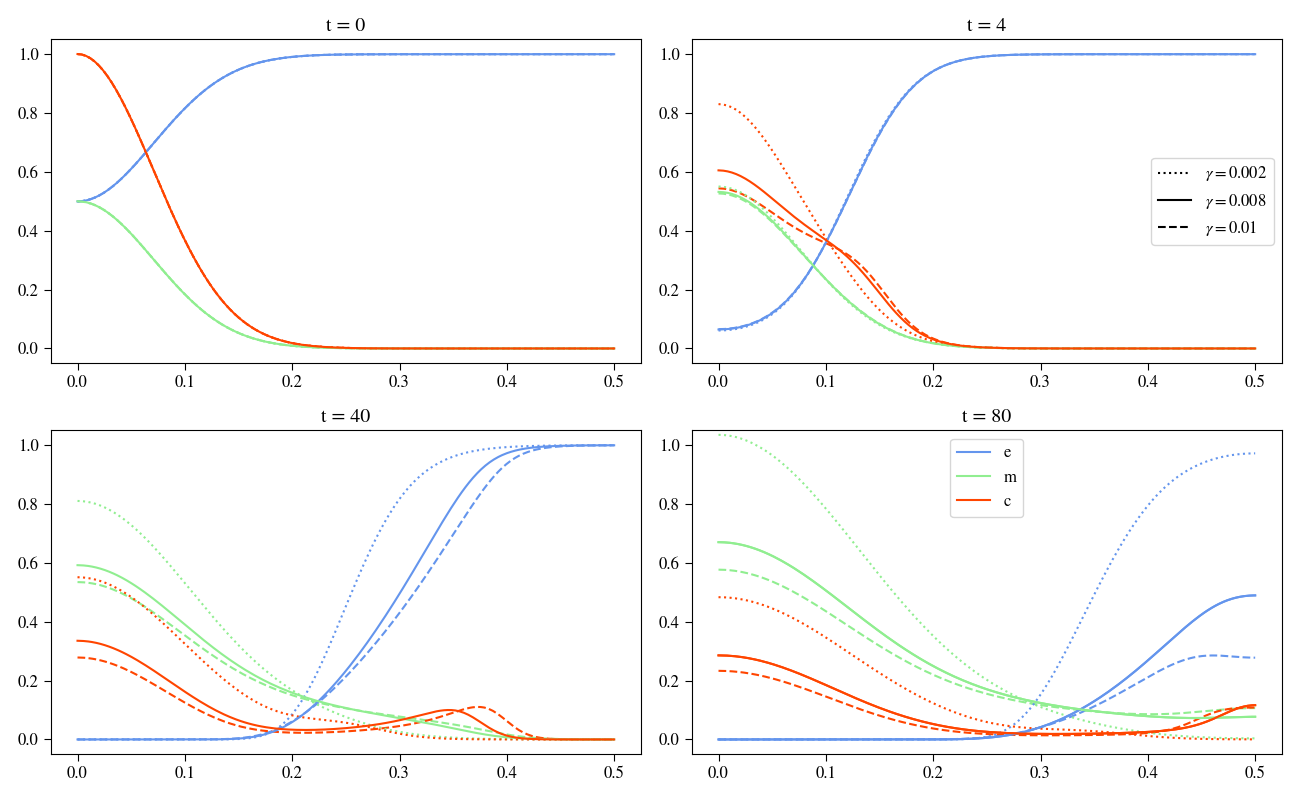
\includegraphics[width=\textwidth]{resources/images/prolif_gamma_variation.png}
    \caption{Plots show results for varying $\gamma$ whilst keeping the other parameters constant.}
    \label{fig:prolif_gamma_variation}
\end{figure}

When we look at $\gamma$ we also can see the same effects as the model without proliferation shows, with the adjustments as varying $d_c$, with raised curves for all variables. Increasing $\gamma$ means increasing haptotaxis effects, pulling the tumor cells stronger towards the extracellular matrix molecules, which causes a faster invasion pace and also a higher density of tumor cells invading the tissue, but a lower staying at the centere at $x=0$. This also means that the ECM degrading process happens faster and the MDEs are more evenly distributed through space the higher $\gamma$ is. As mentioned above the same effects come in this experiment, introducing proliferation and renewal, with higher values for tumor cell density, MDE and ECM concentration especially at the later points in time clearly depictable. It is interessting to observe that though introducing a renewal factor for the extracellular matrix, the proliferation of the tumor cells causes a faster production of matrix-degrading enzymes, which makes the system produce nearly the same results as without proliferation and renewal concerning the ECM concentration, still  it is to say that introducing the renewal of the ECM results in overall slightly higher concentrations of it.

\subsubsection*{$\mu_1$ Variation}
\begin{figure}[h]
    \centering
    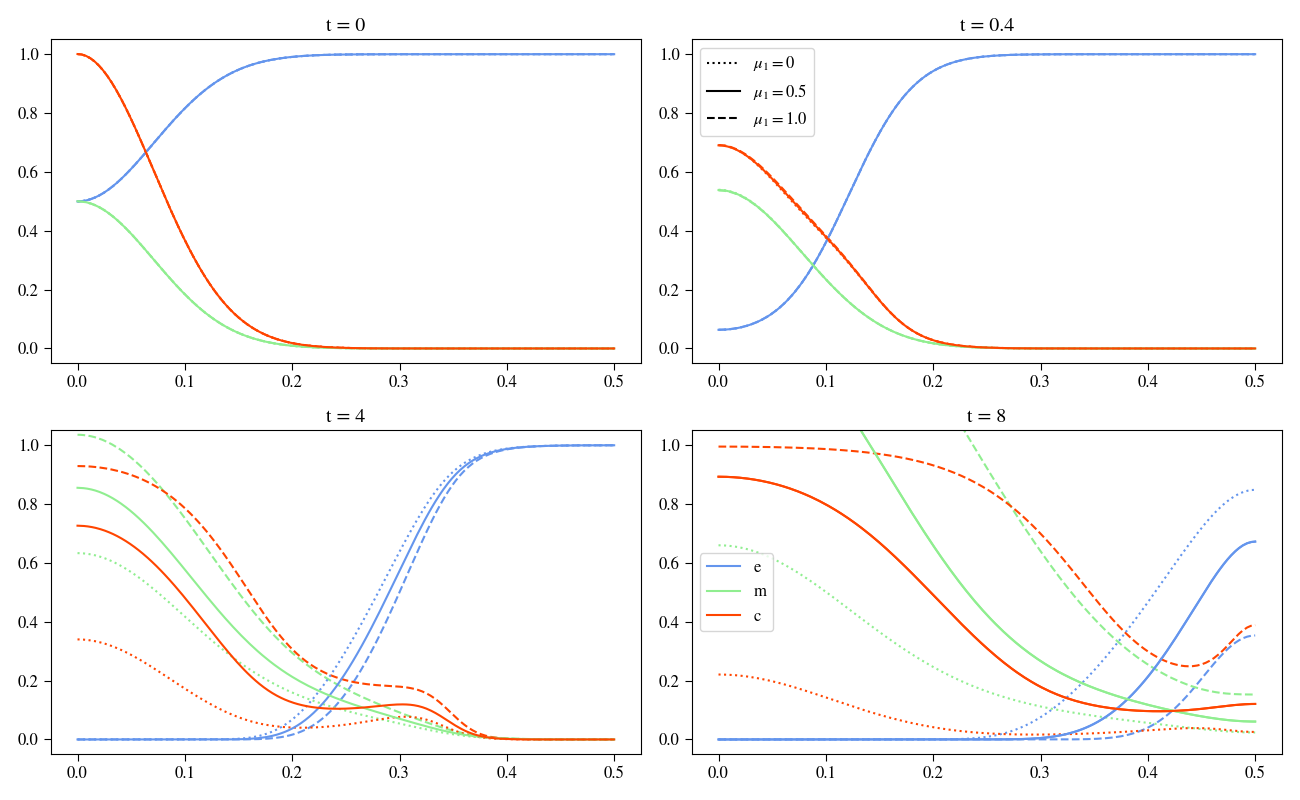
\includegraphics[width=\textwidth]{resources/images/prolif_mu_1_variation.png}
    \caption{Plots show results for varying $\mu_1$ whilst keeping the other parameters constant.}
    \label{fig:prolif_mu_1_variation}
\end{figure}

The parameter $\mu_1$ describes the proliferation of the tumor cells, using Kolev et al's estimate in \cite{Kolev2010} we can assume an even distribution with $\mu_1 \sim U[0.1, 1.0]$. We see that with varying $\mu_1$ the other curves are also strongly influenced though it takes some time as the plots in figure~\ref{fig:prolif_mu_1_variation} indicate, with after $t=0.4$ they seem to overlay each other. At $t=4$ we see that first of all the tumor cells curve obviously increases with increasing $\mu_1$, this causes the MDE concentration to also increase and in turn the ECM curve is decreased due to faster ECM degradation, because of more availabe matrix-degrading enzumes. At the last point in time this befaviour intensifies, the tumor cells having for high $\mu_1$ values a density of one in the range of $x$ being between $0$ and $0.2$ and for $\mu_1=0.5$ also a lot higher than without proliferation of tumor cells. The MDE concentration exceeds one for the two higher values for $\mu_1$ and the ECM having again degraded faster. Looking at the dotted curve, we can observe what only renewal does to our system and we see clearly, comparing it to the basecase of the model without proliferation, that the concentration of the extracellular matrix especially at the end is visibly higher.



\subsubsection*{$\eta$ Variation}
\begin{figure}[h]
    \centering
    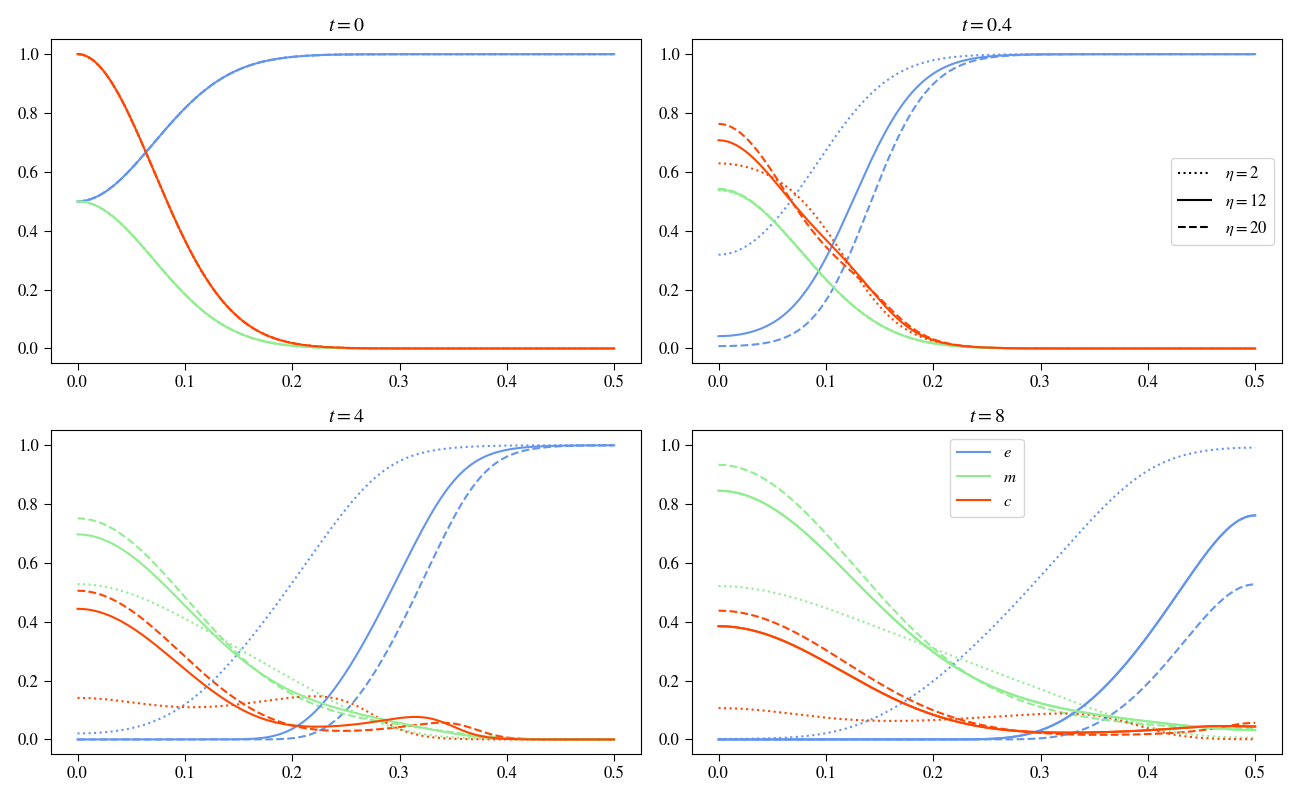
\includegraphics[width=\textwidth]{resources/images/prolif_eta_variation.png}
    \caption{Plots show results for varying $\eta$ whilst keeping the other parameters constant.}
    \label{fig:prolif_eta_variation}
\end{figure}

As we compare the $\eta$ variation between with and without proliferation and renewal models we see mostly the same effects. For the solid and dashed curves we see little though the curves of the new model are all slightly raised. Looking at $\eta=0$ we see some interesting deviations, at the time point $t=0.4$ the plots still look rather similar, but looking at $t=4$ we see that the curve of the tumor cells has a more even distribution along the x-axis and also its maximum is visibly lower with value of about $0.2$ at $x=1.4$ instead of $0.25$ at $x=1.3$. This behaviour is due to the renewal of the ECM, where without proliferation this curve stayed constant throughout the experiment, here it can increase, which it does altering the slope of the curve and therefore influecing the haptotatic pull for the tumor cells, additionally to this the other two experiments showed a visible increase of the tumor cell density and the matrix-degrading enzyme concentration, but only a slight for the ECM concentration, here we can see no increasing of area for the tumor cell density at all. The renewal of the ECM counters the proliferation of the tumor cells and the slowed ECM degrading process in such a way that at the last two point in time we see that the ECM has visibly increased, with both curves ECM and tumor cells almost mirroring each other. Summing up the areas of both variables we see that they toghether occupy the space completely needed for the logistical growth terms, which means that proliferation and renewal will play no more important role continuing with this experiment as they have reached a equlibrium state and cancel each other out. 


\subsubsection*{$\mu_2$ Variation}
\begin{figure}[h]
    \centering
    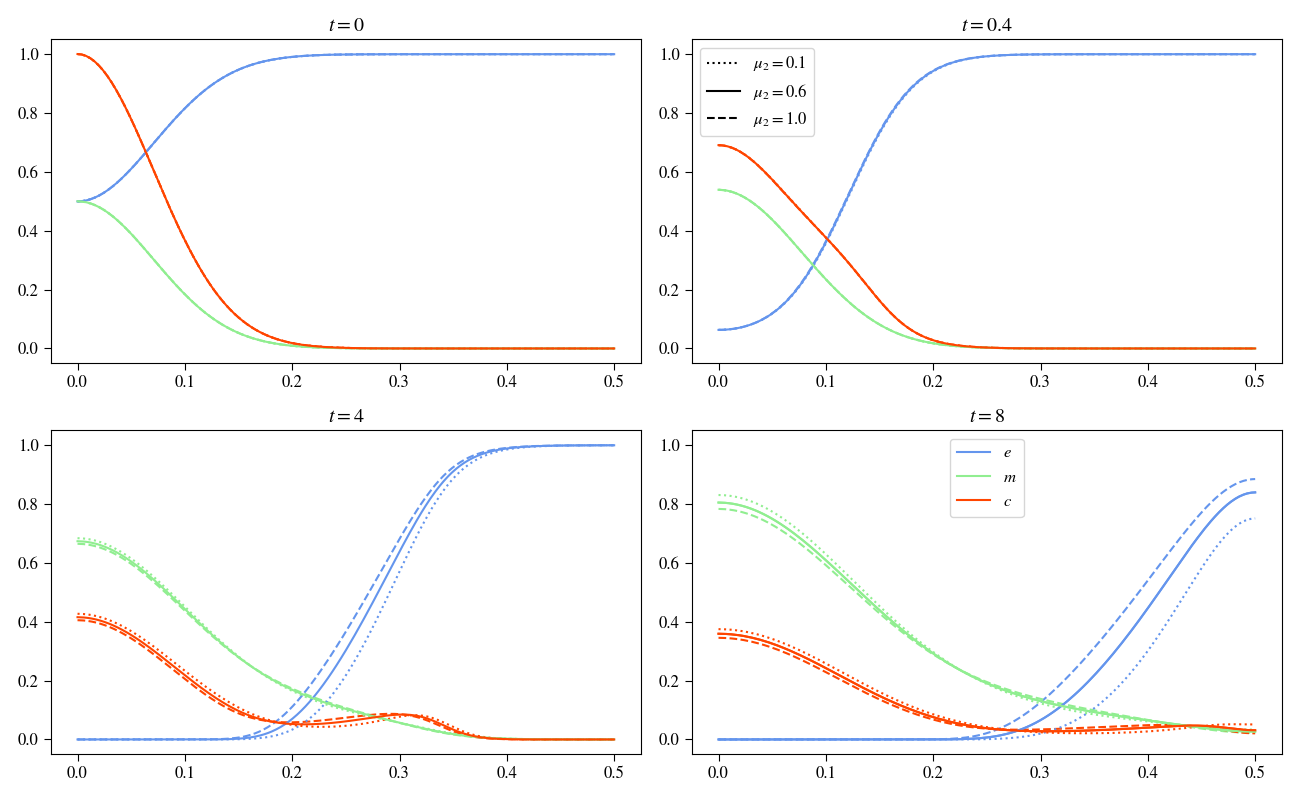
\includegraphics[width=\textwidth]{resources/images/prolif_mu_2_variation.png}
    \caption{Plots show results for varying $\mu_2$ whilst keeping the other parameters constant.}
    \label{fig:prolif_mu_2_variation}
\end{figure}

The parameter $\mu_2$ describes the renewal processes of the extracellular matrix molecules, with also eusing Kolev et al's estimate in \cite{Kolev2010} we can assume an even distribution with $\mu_2 \sim U[0.1, 1.0]$.\newline 
Like we saw for $\mu_1$ the effects of $\mu_2$ need some time to show, here again we can see them after $t=4$ timesteps clearly. Wtih higher ECM renewal we see that we get slightly lower MDE maximum at $x=0$, though having stretched a little more into x-direction. The same goes for the tumor cell density, having a lower maximum at the origin, yet being more evenly distributed, whcih is due to the ECM curve being shifted slightly towards the left, intensifying the effects of haptotaxis. The last image confirms the aforementioned effects with higher ECM concentration due to renewal causes less MDE concentration at its maxima and more stretchig along x-direction, the same holding for the tumor cells. We also observe that the effects of $\mu_2$ are not as impactful on the system as the effects of $\mu_1$ were.

\subsubsection*{$d_m$ Variation}
\begin{figure}[h]
    \centering
    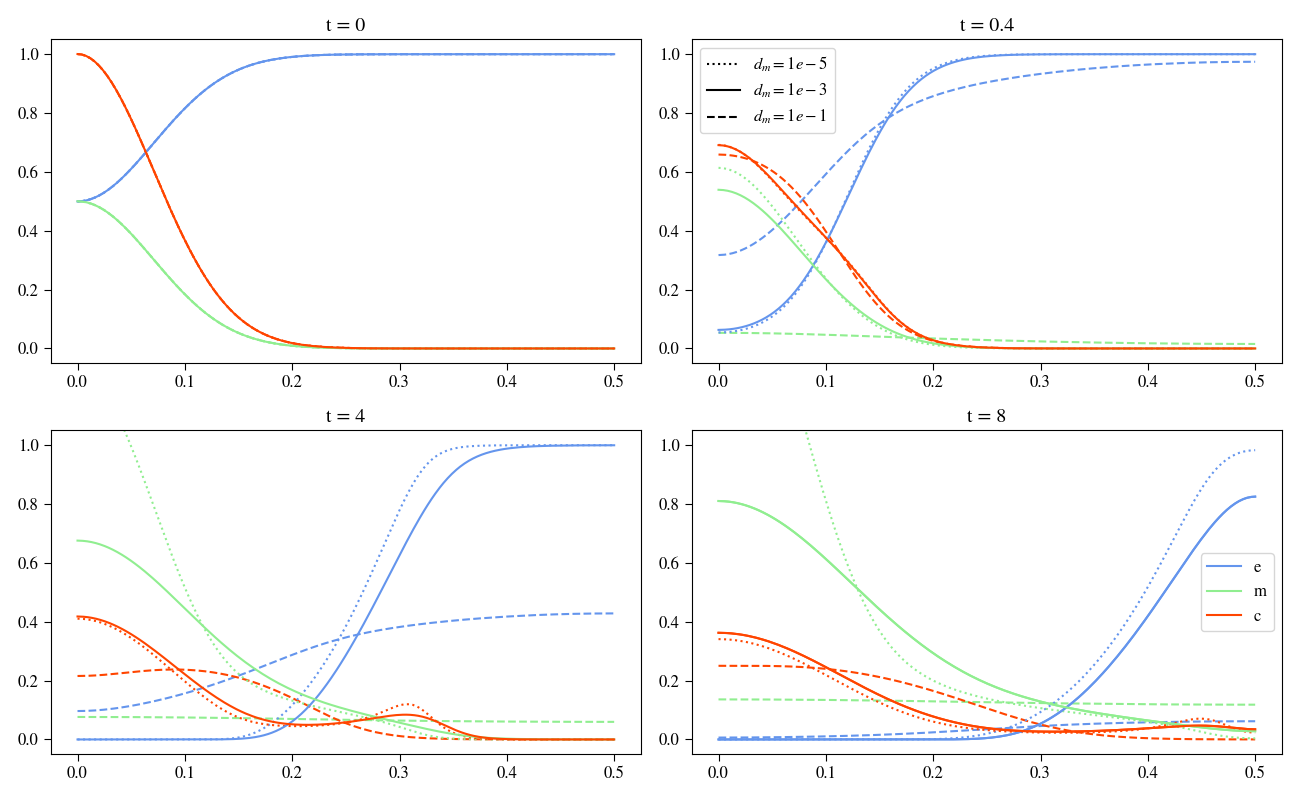
\includegraphics[width=\textwidth]{resources/images/prolif_dm_variation.png}
    \caption{Plots show results for varying $d_m$ whilst keeping the other parameters constant.}
    \label{fig:prolif_dm_variation}
\end{figure}

Comparing the results varying the diffusion factor of the matrix-degrading enzymes does as before yield only minor differences between the initial and updated model. As observed before the tumor cell density's curve and the MDE concentration's curves are slightly raised due to proliferation of the tumor cells. The ECM curve for two lower values of varying $d_m$ though seem to be subject to little to no change, only for very high values of $d_m$ we can see that it is clearly raised comparing it to the model without renewal. The other two curves take off at the some point along the x-axis and finish at the same values for their ECM concentration. Looking at the tumor cell density curves for those $d_m$ values we see that towards $x=0.5$ they don't describe a as steep bump as the initial model. This causes to have little less MDE concentration as well, which is responsible for the seemingly unchanged behaviour of the extracellular matrix concentration.

\subsubsection*{$\alpha$ Variation}
\begin{figure}[h]
    \centering
    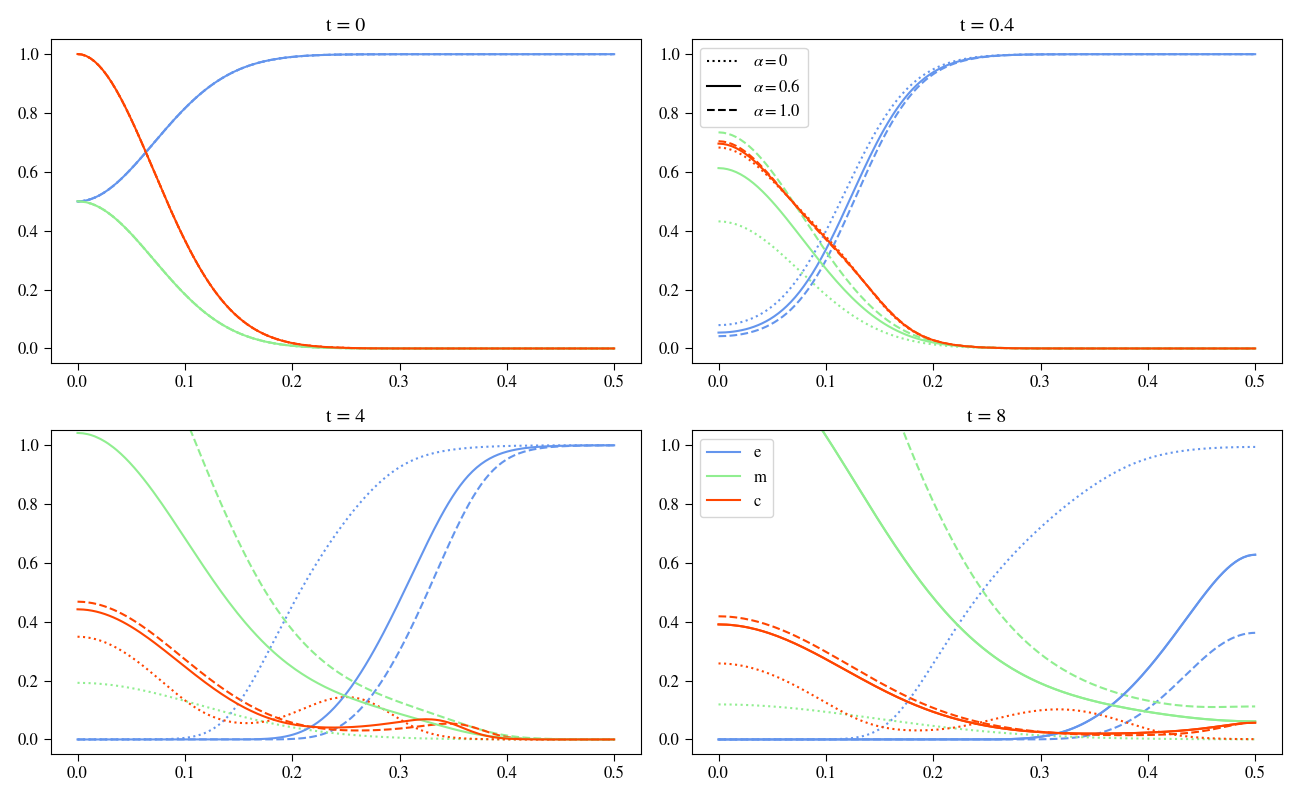
\includegraphics[width=\textwidth]{resources/images/prolif_alpha_variation.png}
    \caption{Plots show results for varying $\alpha$ whilst keeping the other parameters constant.}
    \label{fig:prolif_alpha_variation}
\end{figure}

Taking a look at comparing the $\alpha$-variation yields more interesting results since, $\mu_1$ acts as a secondary MDE production effect by producing tumor cells which in turn produce the matrix-degrading enzymes. We see that though the overall shape and effects to be observed are the same, after $t=4$ the model with proliferation exceeds one at the origin for the MDE concentration for the two higher $\alpha$ experiments, where in the model without proliferation only the one with the highest $\alpha$ value did. The tumor cell denstiy curve is slightly raised, which allows the MDE concentration. Though the higher values for the MDEs leave the ECM degrading process untouched with not clearly visible difference between the inital model and the updated one. 

\subsubsection*{$\beta$ Variation}
\begin{figure}[h]
    \centering
    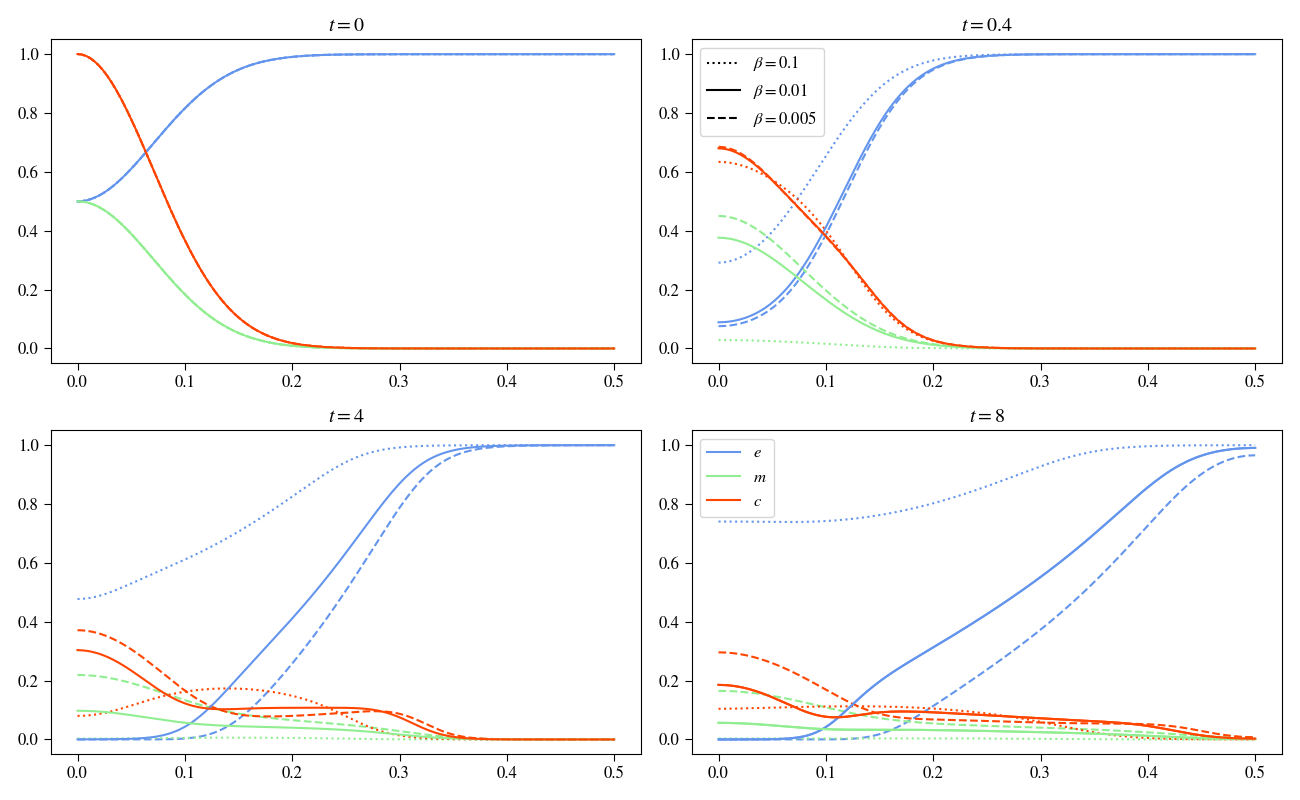
\includegraphics[width=\textwidth]{resources/images/prolif_beta_variation.png}
    \caption{Plots show results for varying $\beta$ whilst keeping the other parameters constant.}
    \label{fig:prolif_beta_variation}
\end{figure}

Considering $\beta$ we can expect that with the introduction of $\mu_2$ the ECM degradation will be slowed considerably with rising $\beta$, since this does not only reduce the MDE concentration but does also renew the ECM. Looking at the plots we can see exactly this behaviour in the dotted line, which shows the experiment results for the highest $\beta$ value of $0.1$. Though even at the end it has an overall area that is slightly less than the inital condition we can see going from timestep $t=0.4$ to $t=4$ that MDE decay and ECM renewal were sufficiently strong to restore the ECM and going from $t=4$ to $t=8$ we see this behaviour again, renewing the ECM. The other two experiments for $\beta$ showed no effects as strong as with $\beta=0.1$, yet we can still see the effects of proliferation and renewal especially clear in the solid line, $\beta=0.01$ at the last point in time, where we can observe a visible increase of both ECM and tumor cell density. In this experiment we see that $\beta$ is a little too low to counter the effects of ECM degradation, going from $t=4$ to $t=8$ we see a clear dicline of ECM concentration though it is not as striking as for $\beta=0.005$. 

\subsubsection*{Cross Variation}

\subsubsection*{$\mu_1 - \mu_2$ Variation}
\begin{figure}[h]
    \centering
    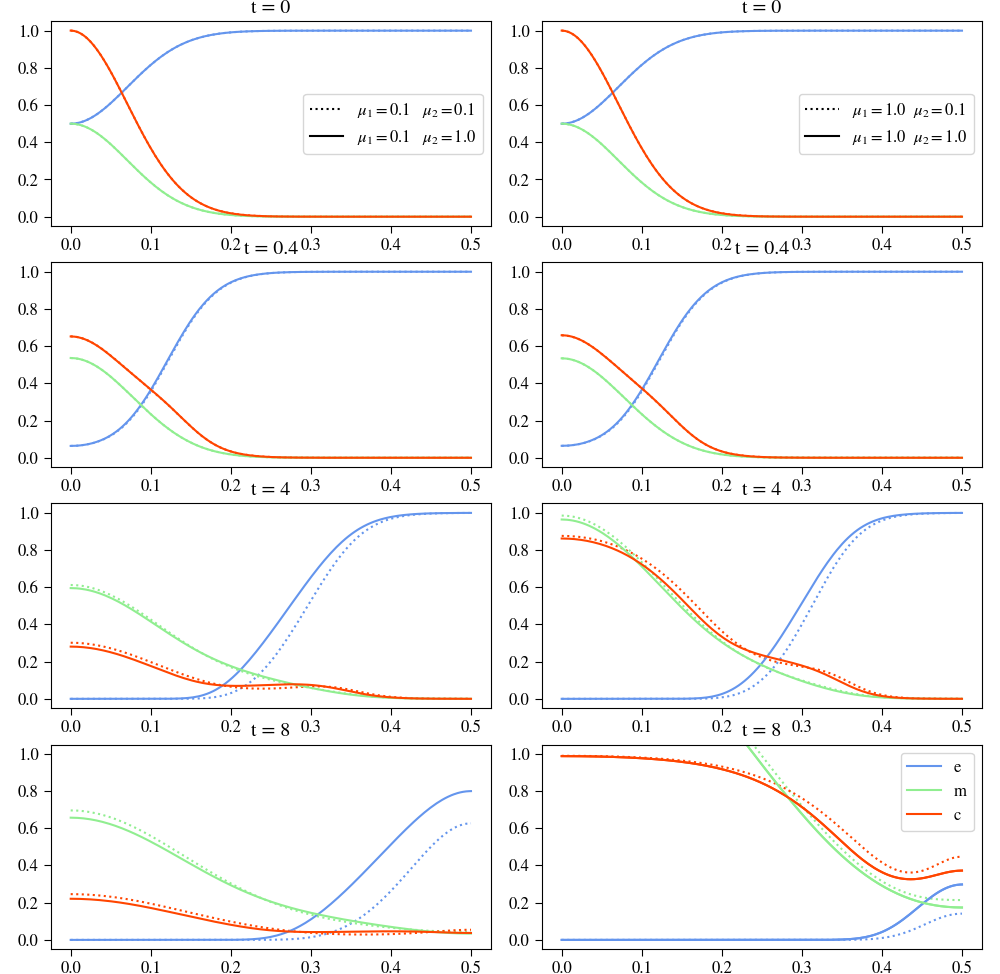
\includegraphics[width=0.85\textwidth]{resources/images/prolif_mu_1_mu_2_variation.png}
    \caption{Plots show results for varying both $\mu_1$ and $\mu_2$ whilst keeping the other parameters constant.}
    \label{fig:prolif_mu_1_mu_2_variation}
\end{figure}
The effects to observe in this cross variation take some time as did the seperate variations of both $\mu_1$ and $\mu_2$. for both $\mu_1=\mu_2=0.1$ we see that slower ECM renewal and slower tumor ell proliferation increase the degrading process of the extracellular matrix and with this affect the haptotaxis effect to increase slightly. At the center a lump remains that has a maximum a little higher than for the experiment with $\mu_2=1.0$ and also the invasion of the tissue has proceeded a little faster. Increasing $\mu_2$, as previously mentioned, results in slower ECM degradation due to the increased renewal term and therefore the tumor cells are stretched out more evenly along the x-axis. Looking at the results when incresing $\mu_1$ we also see the effects only after $t=4$. For $\mu_2=0.1$ we see that the tumor cell density at $x=0$ is slightly larger as well as at $x\approx 2.9$ the curve for $\mu_2=0.1$ is also slightly larger being a little below $\mu_2=1.0$ in between $x\approx 0.2$ and $x\approx 0.29$. The curve for the MDEs looks very similar in both cases for $\mu_2$ due to the very similiar tumor cell density curve, c, though th eECM has visibly faster degraded for $\mu_2=0.1$ due to the slower renewal.

\subsubsection*{$d_c - \gamma - \mu_1$ Variation}
\begin{figure}[h]
    \centering
    \adjustbox{width=0.85\textwidth}{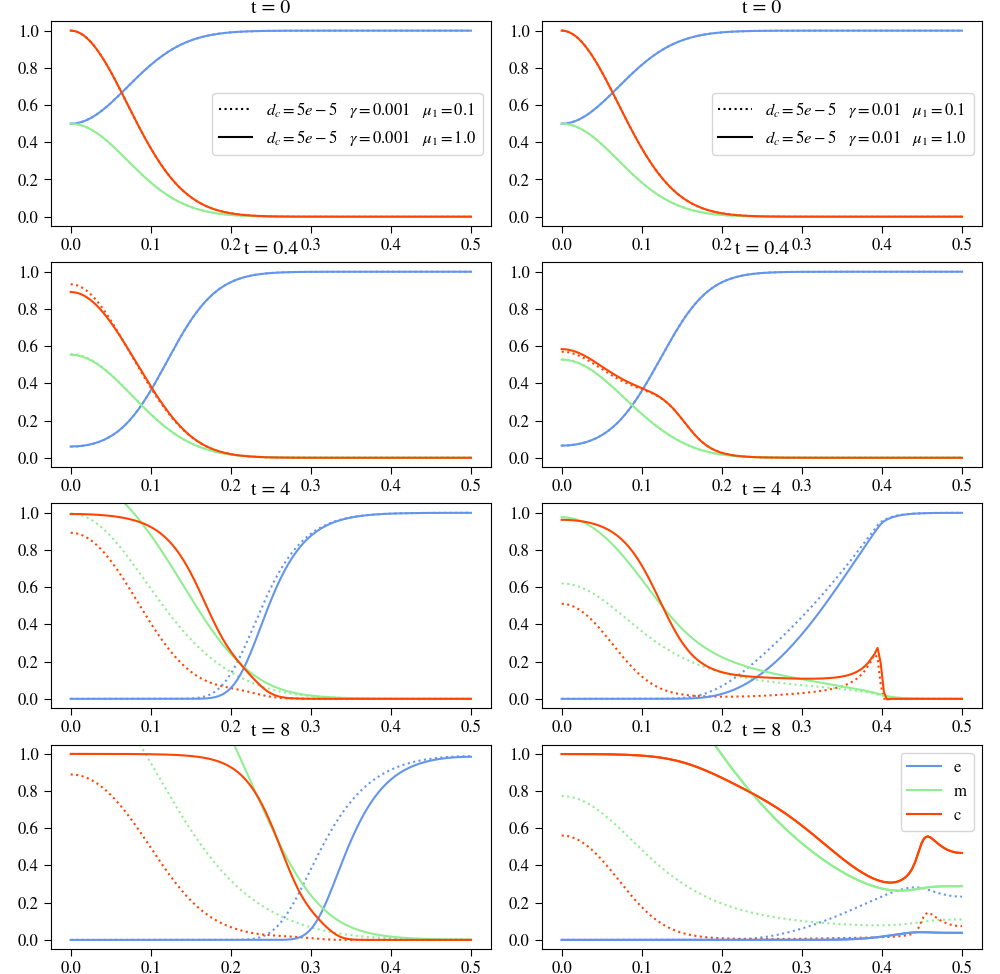
\includegraphics{resources/images/prolif_dc_gamma_mu1_1.png}}
    \caption{Plots show results for varying both $d_c$, $\gamma$ and $\mu_1$ whilst keeping the other parameters constant. This plot is the first of two, with the same $d_c$ value for every plot in this figure.}
    \label{fig:prolif_dc_gamma_mu_1_variation_1}
\end{figure}

\begin{figure}[h]
    \centering
    \adjustbox{width=0.85\textwidth}{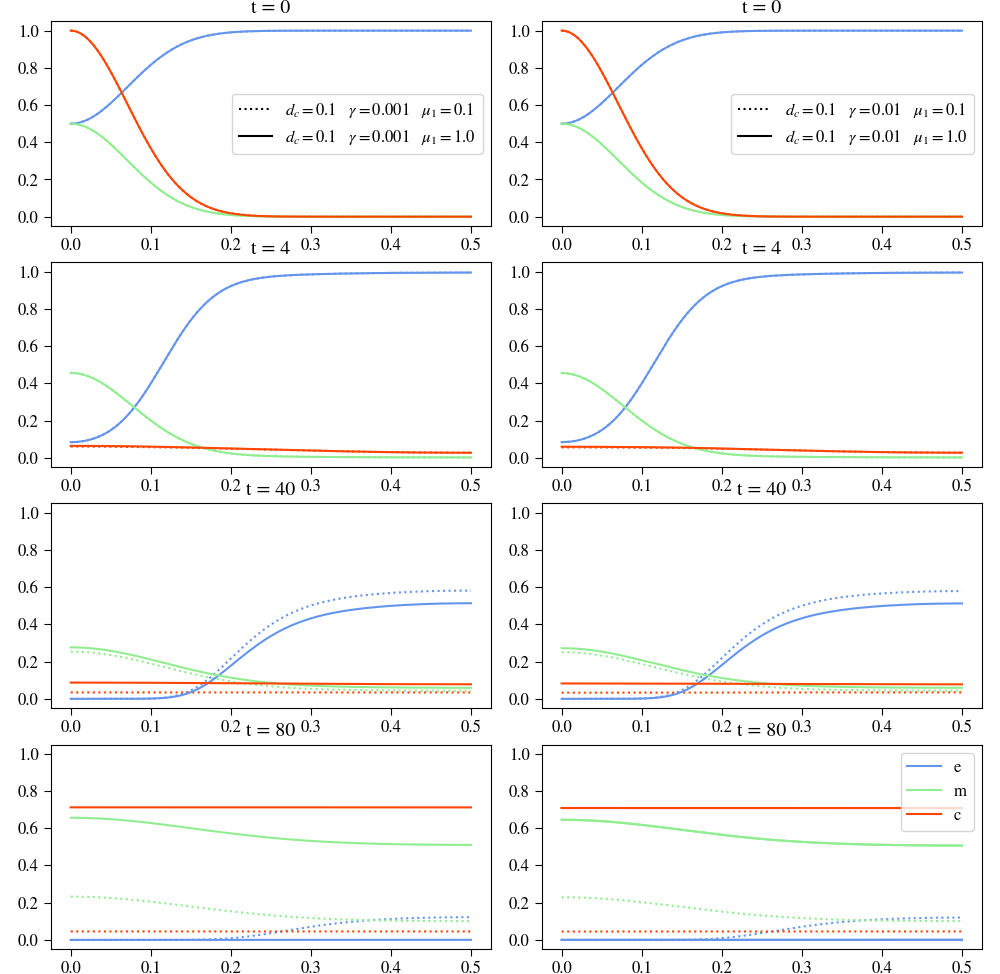
\includegraphics{resources/images/prolif_dc_gamma_mu1_2.png}}
    \caption{Plots show results for varying both $d_c$, $\gamma$ and $\mu_1$ whilst keeping the other parameters constant. This plot is the second of two, with the same $d_c$ value for every plot in this figure.}
    \label{fig:prolif_dc_gamma_mu_1_variation_2}
\end{figure}

First we are goint to take a look at how chaning $\gamma$ and $\mu_1$ affects the system whils having low diffusion values for the tumor cells with $d_c=0.00005$, in figure~\ref{fig:prolif_dc_gamma_mu_1_variation_1}. Inspecting the dotted curve on the left side column, shows the results for all parameters set to low, we see that diffusion is tha mian factor for the movement of the tumor cells, with only little influence of haptotaxis, the tumor cells staying with their maximum at the center. Becasue fo this we also get a high MDE concentration there, but very little excedding the region past $x=0.3$. Due to the MDE also staying centered around thr origin the ECM there is completely degraded, though at $x=0.4$ and further still completely there. Increasing the proliferation factor to $\mu_1=1.0$ shifts the tumor cell density rightwards, making proliferation also a factor for the cell density movement, though keeping the same shape as the low proliferation factor experiment. This right shift causes the MDE concentration to also shift to the right, leading to a faster ECM degradation. Comparing these two experiments already shows the influence of proliferation.\newline
Taking now a look at the right column in figure ~\ref{fig:prolif_dc_gamma_mu_1_variation_1} we see the effects of increased $\gamma$ to $\gamma=1.0$. Foremost we see for the tumor cell density a leading edge developing, seperating it into two lumps, with one staying at the center the other invading the tissue and staying where $\nabla (c \nabla e)$ is highest. With increased $\mu_1$ this secession moving into the tissue is getting more pointy, defying differentiability. After $t=4$ we can observe clear differences regarding ECM and MDE concentration. We see that for higher $\mu_1$ we also get a higher MDE concentration which degrades the ECM visibly faster at the end of the experiments at $t=8$. Though interestingly at $t=4$ the ECM degradataion difference is only minor, at the last point in time the accellerated tumor cell proliferation shows its effet with producignmore MDEs and degrading the ECM considerably faster. What is also interesting to note is that increasing $\gamma$ and keeping $\mu_1$ low the total area of the MDE concentration is lowered also.
Increasing now $d_c$ to $0.1$ we see for all experiments in figure~\ref{fig:prolif_dc_gamma_mu_1_variation_2} that the diffusion of the tumor cells was sufficiently high to evenly distribute the tumor cells constatnly in the space. This constant distribution allows to get an even better look at how $\mu_1$ affects the results, by seeing the lines, describing the tumor cells, rise through time. Looking at the tumor cells over time we can see no observable difference for varying $\gamma$. Haptotaxis effects are completely overlaid by diffusion. We see in the left column that if keeping dc high and $\gamma$ low, but increasing $\mu_1$ leads to higher MDE production rates and also faster ECM degradation. The same behaviour is observable in the right column showing the results for high $\gamma$. That we see no difference is clear, since the tumor cell density development is identical over time as mentioned above. 



\subsubsection*{$\eta -\mu_2$ Variation}
\begin{figure}[h]
    \centering
    \adjustbox{width=0.85\textwidth}{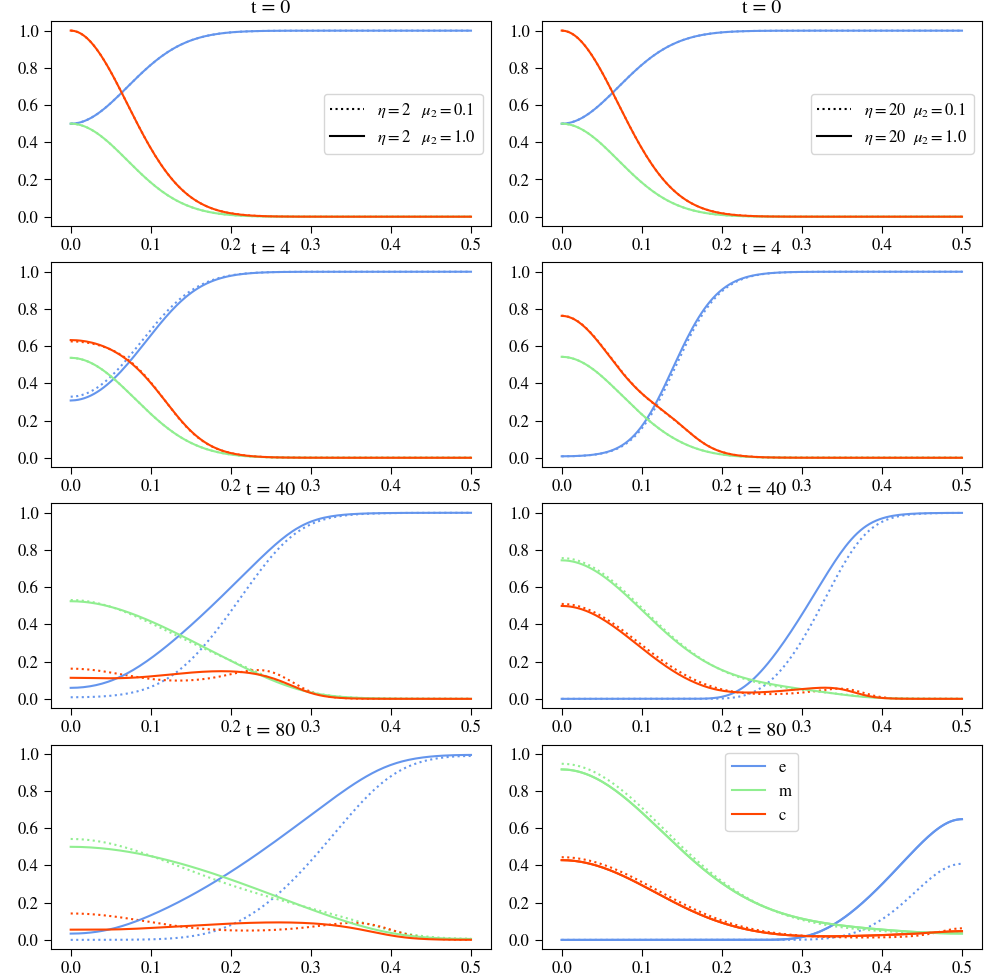
\includegraphics{resources/images/prolif_eta_mu2_variation.png}}
    \caption{Plots show results for varying both $\eta$ and $\mu_2$ whilst keeping the other parameters constant.}
    \label{fig:prolif_eta_mu_2_variation}
\end{figure}

Varying both $\eta$ and $\mu_2$ we can expect to see clear changes in the curve describing the ECM concentration. On the left side of figuer~\ref{fig:prolif_eta_mu_2_variation} we can see the two experiments for low $\eta$ values and see that increasing $\mu_1$ has only a little effect. Where we could have expected to maybe even see an increase of the ECM we see that the ECM curves for both experiments verify that the renewal factor $\mu_2$ was too low to counter the ECM degradation, even with a low degradation factor. Still between $\mu_2=0.1$ and $\mu_2=1.0$ there are visibe differences in the degrading speed of the ECM. We can also observe that with the higher renewal term the tumor cell density curve receives more of an effect of haptotaxis resulting in an more streteched curve with only one long lump of tumor cells, where for the lower renewal factor we can still clearly see that there is a secession that invades the tissue and one that stays at the origin. Concerning the MDE curves we can see little difference, for higher $\mu_2$, which meant more stretched tumor cell density, we can also observe a more stretched MDE curve with a lower maximum at the origin. \newline 
Taking now a look at the experiments with raised $\eta$ to accellerate the ECM degrading process, we can only see pregnant differences in the curve describing the ECM concentration, the other two look across the steps in time to be widely similar. For the ECM curve we see that the experiment with the lower $\mu_2$ value results in a faster degradation process.




\subsection{Three Dimensional Results with Proliferation and Renewal}
\lipsum[1-3]




\subsection{Heterogenous ECM Structure}
\begin{figure}[h]
    \centering
    \label{fig:Initial_Value_Distribution}
    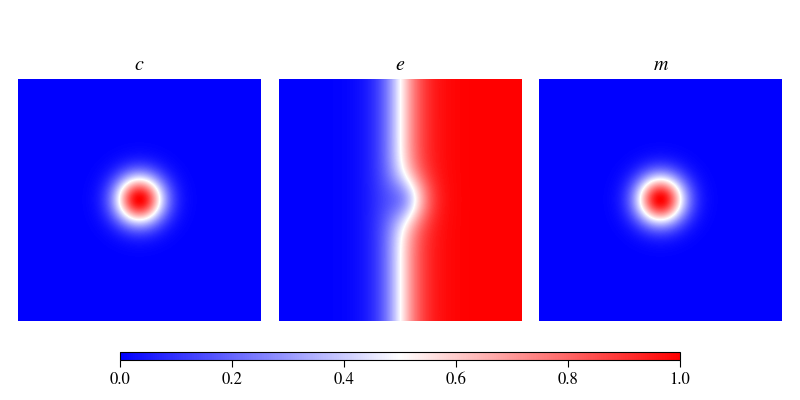
\includegraphics[width=0.8\textwidth]{resources/images/2D_initial_conditions_heterogenous_ECM.png}
    \caption{Visualization of the initial value distribution for an experiment in two space dimensions with a heterogenous extracellular matrix}
    \label{fig:2D_heterogenous_ECM_initial}
\end{figure}
In this section we are investigating how a more realistic structure of the ECM will affect the results of a simulation. We are still using the model with proliferation and renewal. 
For this scenario we assume that there is a nodule of tumor cells already in the center of the simulation that has produced a concentration of matrix-degrading enzymes. Contrary to previous experiments we are assuming that the tumor cells are located at a basement membrane that they already have invaded and are now pushing into the extracellular matrix that lies behind it. These assumptions are described in figure~\ref{fig:tumour_invasion_stage}. We model this in the following experiment with the initial conditions:
\begin{align*}
    c(x,0)= \exp(\frac{-(x-0.5)^2}{0.01})
\end{align*}
\begin{align*}
    m(x,0) = 0.5 c(x,0) = 0.5 \exp(\frac{-(x-0.5)^2}{0.01})
\end{align*}
\begin{align*}
    e(x,0) = 1 - 0.5 c(x,0)
\end{align*}
$\textcolor{red}{insert correct ecm description}$

\begin{figure}[h]
    \centering
    \adjustbox{width=0.8\textwidth}{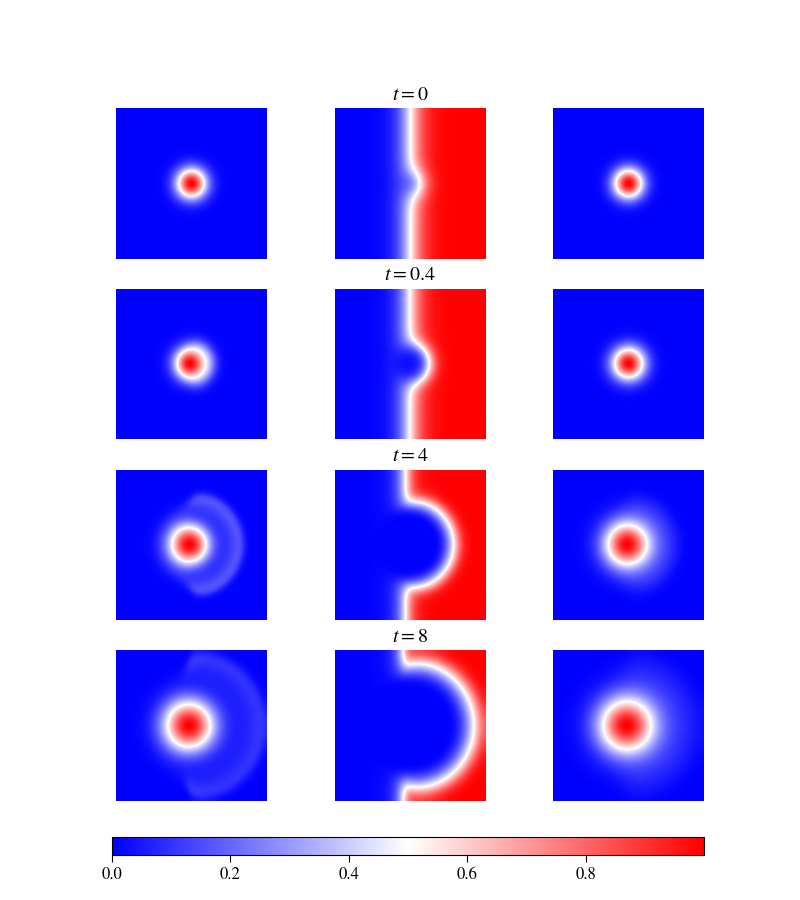
\includegraphics{resources/images/2D_heterogenous_ECM.png}} 
    \caption{2D Results using a heterogenous ECM with the parameter values: $d_c=5\cdot 10^{-4}$, $\gamma=0.0055$, $\mu_1 = 0.1$, $\eta=10$, $\mu_2=0.5$, $d_m = 1\cdot 10^{-3}$, $\alpha = 0.3564$, $\beta = 0$; left: tumor cell density, middle: ECM concentration, right: MDE concentration.}
    \label{fig:2D_heterogenous_ECM}
\end{figure}
Figure~\ref{fig:2D_heterogenous_ECM} you can see the effects using a heterogenous extracellular matrix structure. The plots show in the left column the tumor cell density, the middle column the extracellular matrix concentration and on the right the matrix-degrading enzymes concentration. For the parameters we assumed the basecase studying the model with proliferation. \newline
This experiment describes a more realistic biological scenarino, like seen in figure~\ref{fig:tumour_invasion_stage}, where the tumor cells are located at the basement membrane of neighboring tissue and have degraded this membrane to invade the surrouding tissue and degrade extracellular matrix there.\newline
In the middle column's first image showing the inital distribution of the experiment you see that the extracellular matrix molecule concentration is only on the right side of the plot, this indicated the neighboring tissue to be invaded. In the center of the same image there is hollow spot where the tumor cells of the initial distribution are located. \newline 
After four timesteps you see that the ECM is slowly being degraded and the tumor cells are being pulled by the ECM concentration further into the neighboring tissue. The concentration of the matrix-degrading enzymes shows little differences comparing their behaviour to the experiments done with a homogenous ECM. They only depend indirectly on the ECM, by being produced where the tumor cells are being pulled by the extracellular matrix concentration. \newline
The next point in time shows increased ECM degradation with also further invading tumor cells into the tissue. The tumor cells behave as a semicircular wave moving into the direction of the ECM, you can see the main lump remains at the center, with the edge of having containinig a smaller amount of cells moving outwards. The image describing the matrix-degrading enzyme concentration shows still only minor effects, looking closely we can see that from the center moving to the right there is a slightly higher concentration of them than in the other direction.\newline
The last row depicts the experiment after $t=8$ timesteps and we see the aforementioned effects propagated. The ECM degradation has continued as well as the invasion of the tumor cells. The wave moving in direction of the remaining extracellular matrix molecules has spread through space and therefore decreased in its strength. The MDEs still show only little influence of the heterogenous ECM with the main lump staying centered and only difficult to recognize more concentration towards the movement of the tumor cells and concentration of the extracellular matrix.\newline 
Taking into account different extracellular matrix molecules and structure or physical influences as heat or radiation you can adjust the structure of the ECM and the behaviour of the system to better simulate reallife scenarios of cancer invading tissue.
\section{Conclusion and Discussion}
In this study, we conducted a parameter analysis for a numerical model in tumor development research. The aim was to investigate the impact of varying model parameters and dimensions on simulation outcomes and provide insights into the model's behavior under different conditions. This was done to facilitate implementing this model in a real-world scenario, facilitating an entry point for researchers to choose the parameters for their scenario.

The results of our analysis highlight the model's sensitivity to changes in key parameters, such as the diffusion coefficients on the tumor cells, the haptotatic coefficients, the proliferation rate of the tumor cells, the degradation rate of the extracellular matrix, and the production and decay rates for the matrix-degrading enzymes. We observed that small variations in these parameters can lead to significant differences in simulation outcomes, indicating the importance of carefully selecting and calibrating model parameters for accurate representation of biological phenomena.

Furthermore, our study revealed the complex interplay between different parameters during cross-variating them and their effects on tumor invasion and extracellular matrix degradation. For example, we found that increasing the haptotatic flux coefficient of the tumor cells is the critical component to controlling how many cells of a tumor invade the surrounding tissue and how many stay at the center of the simulation. Most of the parameters studied increased the invasion pace of the tumor cells and the degradation of the extracellular matrix.

Moreover, the influence of spatial dimensions on simulation outcomes was shown, with simulations in higher dimensions producing qualitatively different results compared to the initial one-dimensional model. This underscores the importance of considering the spatial complexity of biological systems when designing computational models for tumor development.

Additionally, our analysis sheds light on the limitations of the current model and areas for further improvement. The model could be extended in both discrete and continuous ways, for example, by implementing biochemical effects like chemotaxis, which is done in Kolev et al.'s work~\cite{Kolev2010} or implement immune cell interactions or heterogeneity in tumor cell populations, to capture the complexity of the tumor microenvironment better.

In conclusion, our parameter analysis provides valuable insights into the behavior of the investigated numerical model in tumor development research and underscores the importance of parameter selection and model validation in mathematical oncology. By refining our understanding of the underlying mechanisms driving tumor progression, such models have the potential to inform therapeutic strategies and improve patient outcomes in the fight against cancer.

\printbibliography
%\end{multicols}
\end{document}